% !TEX root = MemoriaVGalilea.tex
% !TEX encoding = UTF-8 Unicode
% !TEX TS-program = pdflatex
% !TEX spellcheck = Spanish
%
%%%%%%%%%%%%%%%%%%%%%%%%%%
%----- VERSION: 9-10-20215
%%%%%%%%%%%%%%%%%%%%%%%%%%
%
\documentclass[12pt,a4paper,spanish]{book}
%
\usepackage[spanish]{babel}
\usepackage[T1]{fontenc}
\usepackage{lmodern}
\usepackage[utf8]{inputenc}
%
%%%%%%%%%%%%%%%%%%%%%%%%%%%%%%%%%%%%%%%%%%%%%%%%%%%%%%%%%%%%%%%%%%%
%
% Para controlar el tamaño de las hojas y del texto impreso
% Tamaño sugerido por el Servicio de Publicaciones de la UR
%
%%%%%%%%%%%%%%%%%%%%%%%%%%%%%%%%%%%%%%%%%%%%%%%%%%%%%%%%%%%%%%%%%%
\usepackage{geometry}
\geometry{twoside,
  paperheight =297mm,% 24.0cm
  paperwidth = 211mm,%17.0cm
  columnsep = 1.0cm, % Separación cuando haya dos columnas
  textheight = 237mm,%19.0cm,
  textwidth = 166mm, %12.8cm,
  %centering,
  right=20mm,
  left=25mm,
  top = 3.0cm
}
%
%%%%%%%%%%%%%%%%%%%%%%%%%%%%%%%%%%%%%%%%%%%%%%%%%%%%%%%%%%%%%%%
%
% El primer \setcounter es para añadir numeraciones
% a las subsecciones:
%   The sectional levels are numbered starting from 0:
%     \part is level -1
%     \chapter is level 0
%     \section is level 1
%     \subsection is level 2
%     \subsubsection is level 3
%     \paragraph is level 4
%     \subparagraph is level 5
% (el primer 4 hace referencia al nivel 3 (subsubsección)
% y el segundo es para que salga en el toc (table of contents)
%
%%%%%%%%%%%%%%%%%%%%%%%%%%%%%%%%%%%%%%%%%%%%%%%%%%%%%%%%%%%%%%%
%
\setcounter{secnumdepth}{4}
\setcounter{tocdepth}{4}
%
%%%%%%%%%%%%%%%%%%%%%%%%%%%%%%%%%%%%%%%%%%%%%%%%%%%%%%%%%%%%%%
%
% ----- PAQUETES -----
%
%%%%%%%%%%%%%%%%%%%%%%%%%%%%%%%%%%%%%%%%%%%%%%%%%%%%%%%%%%%%%%%
\usepackage{amsmath} % AMS--LATEX
\usepackage{amssymb} % Simbolos del AMS--LATEX
\usepackage{pdfpages} % Para insertar PDF
\usepackage{graphicx}
\usepackage{float} % Para la opción [H] en figuras
\usepackage{tikz}
%
%% Para insertar una figura al lado de un texto:
%\usepackage{wrapfig}
%%
% Si queremos que se añada una sangria en los primeros parrafos cuando trabajamos en ingles, podemos usar el paquete {indentfirst}:
%\usepackage{indentfirst}
%
%\usepackage{color}
%
% Paquete para añadir navegabilidad, pero en el PDF, no en div!
\usepackage{hyperref}
%
% Paquete showkeys para mostrar las etiquetas:
% solo para version preliminar.
% Añadir el paquete despues del paquete hyperref para que tenga
% el efecto completo
%\usepackage[notref,color]{showkeys}
%\usepackage[notcite,notref]{showkeys} % es otra opcion
%
% Paquete para mostrar en la bibliografia las paginas donde
% se citan las referencias
%\usepackage{backref}
%
\usepackage{url} % Para escribir direcciones web
%
%\usepackage{multicol}
%
%%%%%%%%%%%%%%%%%%%%%%%%%%%%%%%%%%%%%%%%%%%%%%%%%%%%%%%%%%%%%%
%
% ----- Nuevo formato para el titulo <Indice General> ------
%
%%%%%%%%%%%%%%%%%%%%%%%%%%%%%%%%%%%%%%%%%%%%%%%%%%%%%%%%%%%%%%
%
%\addto\captionsspanish{%
%\renewcommand{\contentsname}{Contenidos}}
%
%%%%%%%%%%%%%%%%%%%%%%%%%%%%%%%%%%%%%%%%%%%%%%%%%%%%%%%%%%%%%%
%
% ----- Encabezamientos para documentos tipo libro -----
%
%%%%%%%%%%%%%%%%%%%%%%%%%%%%%%%%%%%%%%%%%%%%%%%%%%%%%%%%%%%%%%
%
% ----------------------------------------------------------
%    Evita las hojas en blanco con encabezamiento cuando
%    se utiliza la opción 'twoside', predeterminada en la
%    clase 'book'.
%    Véase 'Page headers and footers in LaTeX' de
%    Piet van Oostrum (p. 13-14)
% ----------------------------------------------------------
%
\makeatletter  % '@' es ahora una "letter" normal para LaTeX
\def\cleardoublepage{\clearpage\if@twoside\ifodd\c@page\else
    \hbox{}
    \vspace*{\fill}
    \vspace{\fill}
    \thispagestyle{empty}
    \newpage
    \if@twocolumn\hbox{}\newpage\fi\fi\fi}
\makeatother  % '@' se restaura como un caracter 'non-letter'
%
% ----------------------------------------------------------
%    Se redefine "myheadings" pagestyle
% ----------------------------------------------------------
%
\makeatletter  % '@' es ahora una "letter" normal para LaTeX
\renewcommand{\ps@myheadings}{%
    \renewcommand{\@oddhead}{%%% encabezamiento (pag. impar) %%%
       \parbox{\textwidth}{%%% introduce el titulo de la seccion
	           \textsc{\footnotesize\rightmark}\hfill\thepage}}
    \renewcommand{\@evenhead}{%%% encabezamiento (pag. par) %%%
       \parbox{\textwidth}{%%% introduce el titulo del capitulo
            \thepage\hfill\textsc{\footnotesize\leftmark}}}
    \renewcommand{\@oddfoot}{}
    \renewcommand{\@evenfoot}{}
}
\makeatother  % '@' se restaura como un caracter 'non-letter'
%
\pagestyle{myheadings}
%
%
%%%%%%%%%%%%%%%%%%%%%%%%%%%%%%%%%%%%%%%%%%%%%%%%%%%%%%%%%%%%%%
%
% -------------- Definicion de teoremas ---------------
%
%%%%%%%%%%%%%%%%%%%%%%%%%%%%%%%%%%%%%%%%%%%%%%%%%%%%%%%%%%%%%%
%      
\usepackage{amsthm}
%
% Para poner la palabra Proof en negrita y en italica
% (por defecto lo pone solo en italica)
%\let\oldproofname=\proofname
%\renewcommand{\proofname}{\rm\bf\emph{\oldproofname}}
%
% Para poner la palabra Demostracion en negrita y en italica
\addto\captionsspanish{%
\renewcommand{\proofname}{\rm\bf\emph{Demostración.}}}
%
% Para poner como QED un cuadrado negro al final de linea
% (por defecto lo pone blanco)
\renewcommand{\qedsymbol}{$\blacksquare$}
%
%
\theoremstyle{plain}
% en castellano:
\newtheorem{teorema}{Teorema}[chapter]
\newtheorem{lema}[teorema]{Lema}
\newtheorem{proposicion}[teorema]{Proposici\'on}
\newtheorem{corolario}[teorema]{Corolario}
\newtheorem{definicion}[teorema]{Definici\'on}
%
\theoremstyle{definition}
% en castellano:
\newtheorem{ejemplo}[teorema]{Ejemplo}
\newtheorem{algoritmo}[teorema]{Algoritmo}
%\newtheorem{remark}[theorem]{Remark}
%
\theoremstyle{remark}
% en castellano:
\newtheorem{nota}[teorema]{Nota}
%
% Para poner el simbolo \blacktriangleleft al final de ejemplo
\newenvironment{ejemploconqed}[1][]{%
\begin{ejemplo}[#1]
\renewcommand{\qedsymbol}{$\blacktriangleleft$}%
\pushQED{\qed}}%
{\popQED\end{ejemplo}}
%
%%%%%%%%%%%%%%%%%%%%%%%%%%%%%%%%%%%%%%%%%%%%%%%%%%%%%%%%%%%%%%
%
% ----- Definición de comandos -----
%
%%%%%%%%%%%%%%%%%%%%%%%%%%%%%%%%%%%%%%%%%%%%%%%%%%%%%%%%%%%%%%
%
\newcommand{\R}{\mathbb{R}}
\newcommand{\N}{\mathbb{N}}
\newcommand{\C}{\mathbb{C}}
\newcommand{\Z}{\mathbb{Z}}
\newcommand{\Q}{\mathbb{Q}}
\newcommand{\F}{\mathbb{F}}
\newcommand{\e}{\operatorname{e}}
\newcommand{\Fou}{\mathcal{F}(f)}
\newcommand{\sgn}{\operatorname{sgn}}
\newcommand{\Log}{\operatorname{Log}}
%

% Unificar notacion:
\renewcommand{\tan}{\tg} 
\renewcommand{\arctan}{\arctg} 
\renewcommand{\sin}{\sen} 
\renewcommand{\arcsin}{\arcsen} 

\renewcommand{\Re}{\operatorname{Re}}
\renewcommand{\Im}{\operatorname{Im}}


\def\x{x^{\ast}}
\def\z{z^{\ast}}
\def\t{t^{\ast}}
\def\tt{t^{\ast\ast}}
\def\y{y^{\ast}}

%Para ampliar el espaciado entre lineas en una tabla:
\def\espacioextra{&\\[1mm]}	%%%%% IMPORTANTE
\renewcommand{\arraystretch}{0.0}	%%%%% IMPORTANTE
%
%
%%%%%%%%%%%%%%%%%%%%%%%%%%%%%%%%%%%%%%%%%%%%%%%%%%%%%%%%%%%%%%
%
% ----- Para colocar dos figuras en la misma linea -----
%
%%%%%%%%%%%%%%%%%%%%%%%%%%%%%%%%%%%%%%%%%%%%%%%%%%%%%%%%%%%%%%
%
\newcommand{\twofigures}[4]{%
\begin{figure}[htb]
%\setlength{\captionindent}{0pt}
\begin{minipage}[t]{0.47\textwidth}
\begin{centering}
\includegraphics[width=3in, height=3in]{#1}%
\par
\end{centering}
\caption{#2}
\end{minipage}\hfill%
\begin{minipage}[t]{0.47\textwidth}
\begin{centering}
\includegraphics[width=3in,height=3in]{#3}%
\par
\end{centering}
\caption{#4}
\end{minipage}
\end{figure}
}
%
%
%%%%%%%%%%%%%%%%%%%%%%%%%%%%%%%%%%%%%%%%%%%%%%%%%%%%%%%%%%%%%%
%
% -- Para flexibilizar la colocación de figuras y tablas ---
%
%%%%%%%%%%%%%%%%%%%%%%%%%%%%%%%%%%%%%%%%%%%%%%%%%%%%%%%%%%%%%%
%
%\setcounter{topnumber}{4}
%\setcounter{bottomnumber}{4}
%\setcounter{totalnumber}{4}
%\setcounter{dbltopnumber}{4}
%\renewcommand{\topfraction}{.97}
%\renewcommand{\bottomfraction}{.97}
%\renewcommand{\textfraction}{.03}
%\renewcommand{\floatpagefraction}{.9}
%\renewcommand{\dbltopfraction}{.97}
%\renewcommand{\dblfloatpagefraction}{.9}
%\setlength{\floatsep}{12pt plus 6pt minus 4pt}
%\setlength{\textfloatsep}{15pt plus 8pt minus 5pt}
%\setlength{\intextsep}{12pt plus 6pt minus 4pt}
%\setlength{\dblfloatsep}{12pt plus 6pt minus 4pt}
%\setlength{\dbltextfloatsep}{15pt plus 8pt minus 5pt}
%
%
%%%%%%%%%%%%%%%%%%%%%%%%%%%%%%%%%%%%%%%%%%%%%%%%%%%%%%%%%%%%%%
%
\decimalpoint % Español: punto decimal en vez de coma decimal
\renewcommand{\baselinestretch}{1.1} % Entrelineado
%
%%%%%%%%%%%%%%%%%%%%%%%%%%%%%%%%%%%%%%%%%%%%%%%%%%%%%%%%%%%%%%
%
%
%
%%%%%%%%%%%%%%%%%%%%%%%%%%%%%%%%%%%%%%%%%%%%%%%%%%%%%%%%%%%%%%
% --------------------- Titulo y autores ---------------------
%%%%%%%%%%%%%%%%%%%%%%%%%%%%%%%%%%%%%%%%%%%%%%%%%%%%%%%%%%%%%%
%
\title{\textbf{Estudio dinámico de diversos métodos iterativos para resolver ecuaciones no lineales}}
%
\author{Víctor Galilea\\[2ex]
José Manuel Gutiérrez Jiménez\\[2ex]
}
\date{}
%
%
%
\begin{document}
%
% Para que en español ponga Tabbla en vez de Cuadro,
% Referencias en vez de Bibliografia, etc
%\renewcommand{\tablename}{Tabla}
%\renewcommand{\bibname}{Referencias}
%\renewcommand{\listoftables}{Índice de tablas}
%\renewcommand{\appendixname}{Complemento}
%

\frontmatter

\maketitle

%\chapter{Introducción}




\tableofcontents

\mainmatter 

% Cada capítulo aparece en un fichero independiente,
% que no necesita ningún tipo de cabecera,
% pero que debe llamarse igual.

%CAPITULO 1
\chapter{Introducción}

Antecedentes y marco teórico sobre métodos iterativos \cite{Traub} y nociones de dinámica, tanto real como compleja. 1.1. Motivación y relevancia del estudio
1.2. Antecedentes históricos de los métodos iterativos para la resolución de ecuaciones no lineales
1.3. Dinámica compleja y métodos iterativos: una conexión interdisciplinar (topología, análisis numérico, etc.)
1.4. Objetivos de la tesis
1.5. Estructura y organización del trabajo


%CAPITULO 2
\chapter{Fundamentos teóricos}

2.1. Métodos iterativos para la resolución de ecuaciones ( $f(x) = 0 $)
2.2. Teoría de la iteración de funciones racionales
2.3. Conceptos de dinámica compleja: conjuntos de Julia y Fatou
2.4. Conjugación topológica y equivalencia dinámica
2.5. Plano de parámetros y bifurcaciones
2.6. Consideraciones numéricas: convergencia local y global

%%CAPITULO 3
%\chapter{Dinámica del método de Newton}
%
%3.1. Revisión teórica y propiedades fundamentales
%3.2. Dinámica en el plano complejo: cuencas de atracción y fractalidad
%3.3. Dinámica en la recta real
%3.4. Propiedades numéricas: orden de convergencia y estabilidad
%3.5. Discusión sobre su papel como referencia en el análisis comparativo
%
%
%
%\section{Dinámica del método de Newton en el plano complejo}
%
%Aquí se podría seguir el libro de Sergio Plaza
%
%\section{Dinámica del método de Newton en la recta real}

% !TEX root = MemoriaVGalilea.tex
% !TEX encoding = UTF-8 Unicode
% !TEX TS-program = pdflatex
% !TEX spellcheck = Spanish
%
%%%%%%%%%%%%%%%%%%%%%%%%%%
%----- VERSION: 9-10-2025
%%%%%%%%%%%%%%%%%%%%%%%%%%

\chapter[Método de Newton en  el plano complejo]{Dinámica del método de Newton en  el plano complejo} 
\label{capitulo4}



\section{Antecedentes: el problema de Cayley}
\index{Cayley, A.!problema}

\index{Cayley, A.}\index{Schröder, E.}
El estudio de la dinámica del método de Newton en el campo complejo tiene una importancia histórica, desde que E. Schröder (1870) y A. Cayley (1879) propusieran usar el método de Newton para resolver ecuaciones definidas en el plano complejo:
\begin{equation}\label{eq4:1}
f(z)=0, \quad f:\C \to \C.
\end{equation}

\index{Newton, I.!método}
El que se conoce como \emph{problema de Cayley} consiste en estudiar las cuencas de atracción del método de Newton cuando es aplicado para aproximar
las raíces del polinomio complejo  $p(z)$. En palabras del propio Cayley, el problema se puede formular como sigue:
\begin{quote}
<<\dots the problem is to determine the regions of the plane, such that $P$ [initial point] being taken at pleasure anywhere within one region we arrive ultimately at the point $A$ [a root of the polynomial]\dots>>
\end{quote}



Con la notación actual, si $\z$ es una solución de (\ref{eq4:1}), y
\begin{equation}\label{eq4:2}
z_{n+1}=z_n-\frac{f(z_n)}{f'(z_n)}
\end{equation}
es la sucesión generada por el método de Newton a partir de un cierto $z_0\in \C$, se trata de caracterizar la región
$$
A(\z)=\{z_0\in \C: z_n\to \z \},
$$
conocida como \emph{cuenca de atracción} de la raíz $\z$.
Cayley (\cite{Cayley1}, \cite{Cayley2}) consiguió caracterizar los cuencas de atracción de las raíces de un polinomio cuadrático, en concreto del polinomio $p(z)=z^2-1$, aunque fracasó en su intento de extender el estudio al caso cúbico y a grados superiores. Después de un tiempo tratando de resolver el problema para el polinomio cúbico $p(z)=z^3-1$, concluye sus artículos con las  siguientes sentencias:

%\begin{quote}
%<<J'espère appliquer cette théorie au cas d'une équation cubique, mais les calculs sont beaucoup plus difficiles>>
%\end{quote}

\begin{quote}
\guillemotleft The solution is easy and elegant in the case of a quadratic equation, but the next succeeding case of the cubic equation appears to present considerable difficulty (1879).\guillemotright
\end{quote}

\begin{quote}
\guillemotleft The division into regions is made without difficulty in the case of a quadratic equation; but in the next succeeding case, that of a cubic equation, it is anything but obvious what the division is: and the author had not succeeded in finding it. (1880)\guillemotright
\end{quote}




\begin{figure}[htb]
\centering
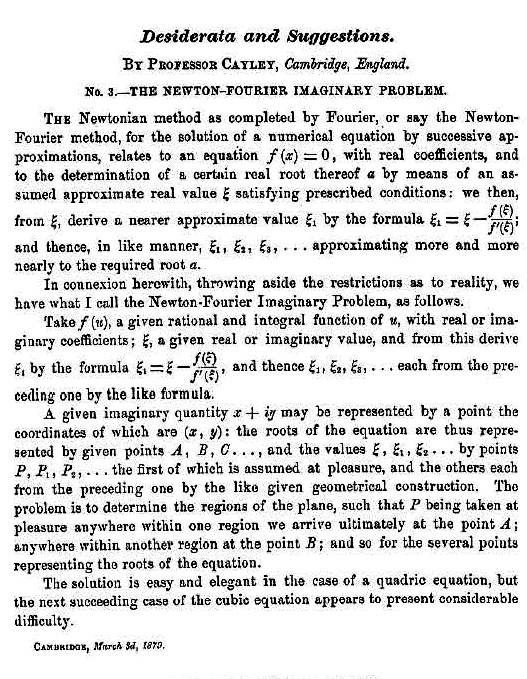
\includegraphics[width=0.45\textwidth]{Cayley1.jpg}
\qquad
 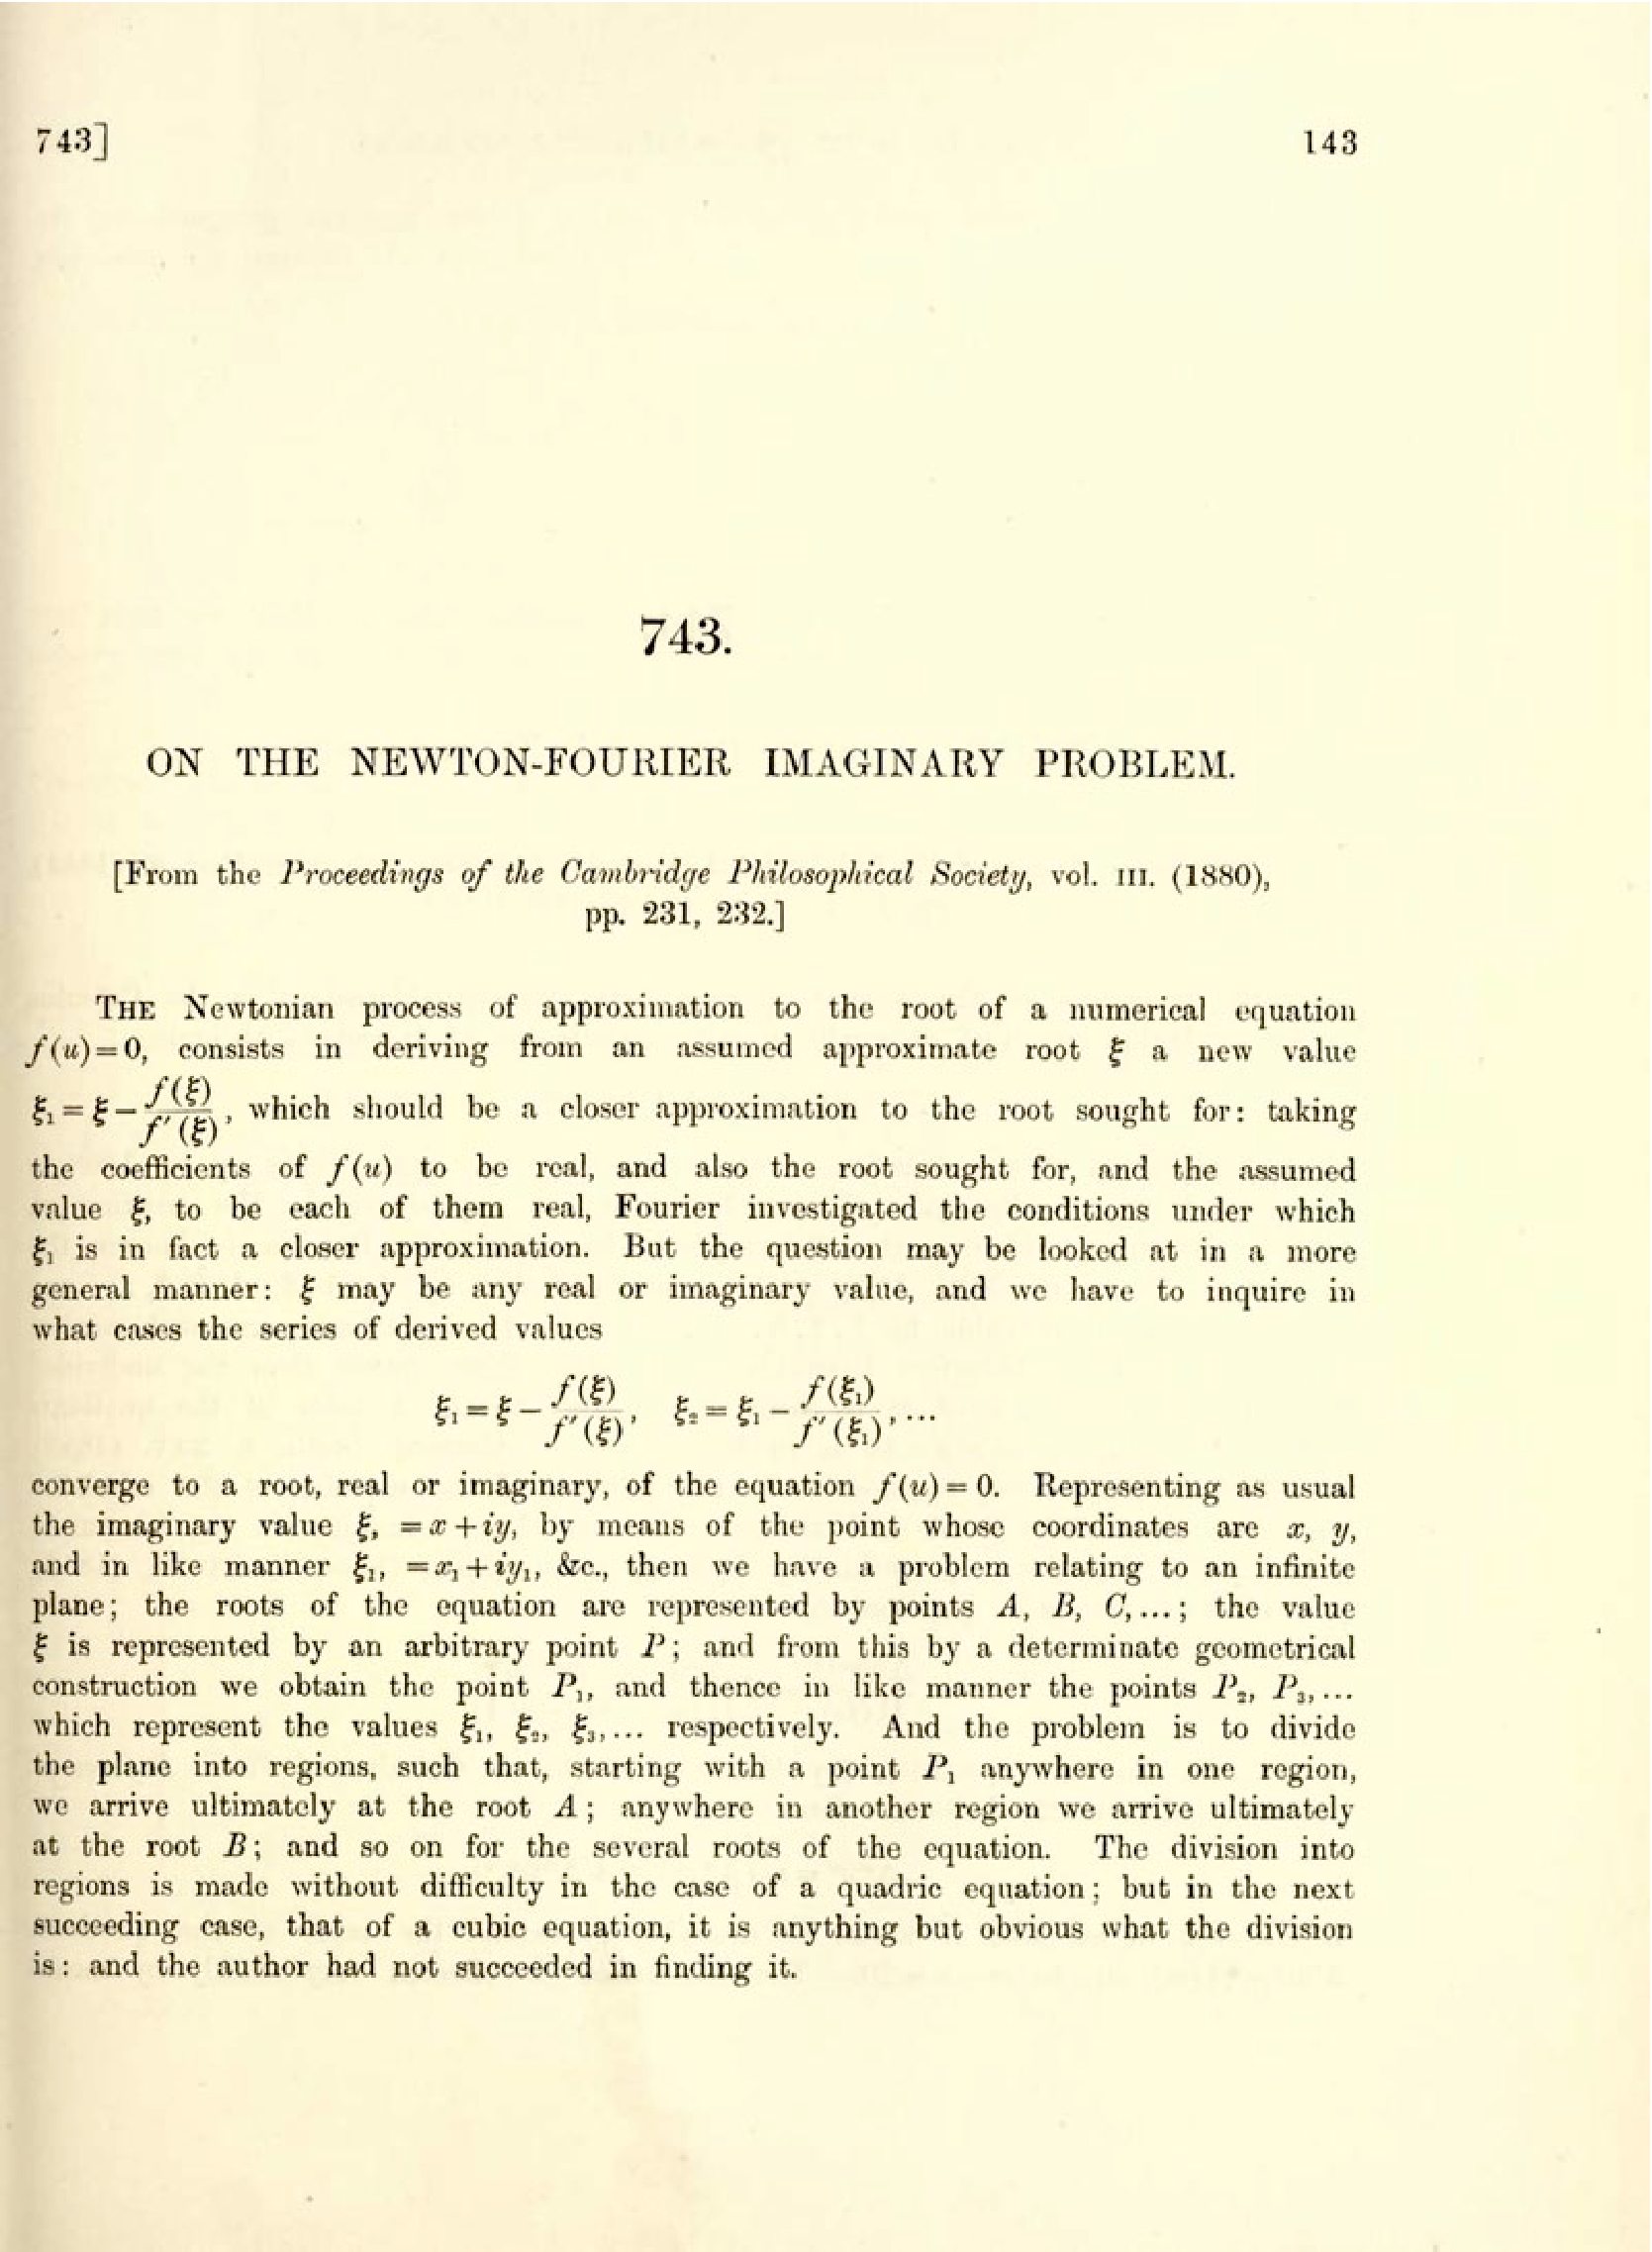
\includegraphics[width=0.45\textwidth]{Cayley2.pdf}
 %\vspace{-1.25cm}
\caption{Los artículos originales de Cayley, de 1879 y 1880 respectivamente,  en los que se pone de manifiesto la dificultad para caracterizar las cuencas de atracción del método de Newton aplicado a polinomios cúbicos.}
 \label{esparam_fig0}
\end{figure}




En la figura~\ref{C4fig:1} mostramos las cuencas de atracción de los polinomios $p(z)=z^2-1$ y $p(z)=z^3-1$. En el primer caso vemos que los puntos de partida situados en el semiplano $\C^-=\{z\in \C: \Re (z)<0 \}$ convergen a la raíz $\z=-1$, mientras que los puntos de partida situados en el semiplano $\C^+=\{z\in \C: \Re (z)>0 \}$ convergen a la raíz $\z=1$. En la separación de ambas regiones, el eje imaginario, en donde el método de Newton presenta un comportamiento caótico. Sin embargo, como vemos en la segunda gráfica de la figura~\ref{C4fig:1}, la situación para el polinomio $p(z)=z^3-1$ es mucho más complicada. La separación entre las cuencas de atracción de las tres raíces, $1$, $(-1+\sqrt{3}i)/2$ y $(-1-\sqrt{3}i)/2$, no es tan diáfana y tiene una estructura mucho más enrevesada.

\begin{figure}[htb]
\centering
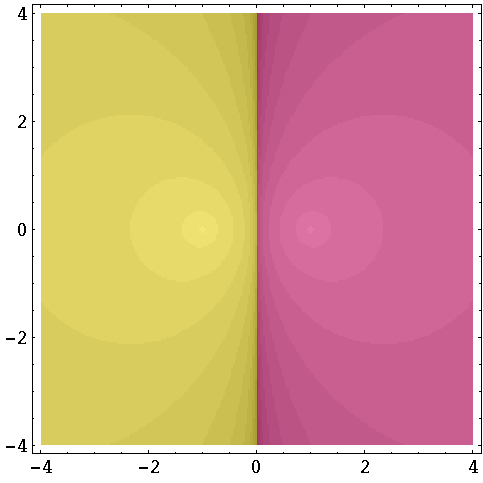
\includegraphics[width=0.45\textwidth]{NDfigura0.pdf}
\qquad
 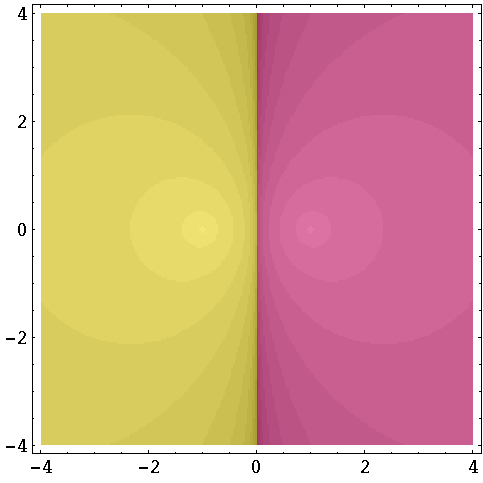
\includegraphics[width=0.45\textwidth]{NDfigura0.pdf}
 %\vspace{-1.25cm}
\caption{A la izquierda se muestran las cuencas de atracción del polinomio $p(z)=z^2-1$ y a la derecha las del polinomio $p(z)=z^3-1$. Las regiones pintadas con el mismo color están formadas por puntos de partida para los cuales el método de Newton converge a la misma raíz del polinomio correspondiente.}
 \label{C4fig:1}
\end{figure}


No es de extrañar, por tanto, que Cayley, que no disponía de los potentes programas de dibujo y cálculo simbólico que tenemos en la actualidad, encontrara dificultades al intentar pasar de una ecuación cuadrática a una cúbica.

Posteriormente, G. Julia y P. Fatou consideran funciones racionales en una forma más general, obteniendo resultados significativos  y sientan el estudio de iteraciones de funciones racionales en el plano complejo extendido, también conocido como la esfera de Riemann. En otras palabras, con sus trabajos comienza en forma sistemática el estudio de los sistemas  dinámicos complejos. La base de sus trabajos fue el estudio realizado por Montel sobre familias normales.%
\index{Fatou, P. J. L.}\index{Julia, G. M.}




\section[Propiedades del método de Newton en $\C$]{Algunas propiedades del método de Newton en el plano complejo} 
\index{Newton, I.!método}

Sea $ p(z) = a_d z^d + \cdots + a_1 z + a_0$, con $ a_d \ne
0$, un polinomio de grado $d $ en $\C$, y sea
$$
N_p(z) = z - \frac{p(z)}{p'(z)} ,
$$
su método de Newton.

Veamos algunas propiedades elementales de la dinámica de
$N_p$:
\begin{itemize}
\item[(1)]  $N_p(z_0) = z_0$ si y sólo si $p(z_0) =  0$,
es decir, los puntos fijos de $ N_p$ son las raíces de~$p$.

\item[(2)]  $ z = \infty$ es siempre un punto fijo de $ N_p$,
y como $   N_p' (\infty) = \frac{d}{d-1}$ este punto fijo es
repulsor. Por lo tanto, si el método de Newton produce un punto
cerca de $ \infty$, sus sucesivas iteraciones se aproximan a
una parte compacta de $\C$.

\item[(3)]  Puesto que $N_p'(z) = \frac{p(z) p''(z)}{(p(z))^2}$,
si $ z_0$ es una raíz simple de $p$,  se tiene que
$ N_p'(z_0) = 0$, esto es, $ z_0$ es un punto fijo
superatractor de $N_p$, lo cual implica que $ N_p$ es
conjugada a la aplicación $ z \to z^k$, para algún $k >
1$ en una vecindad de $z_0$.

\item[(4)]  Las raíces múltiples de $p$ son puntos fijos atractores,
pero no superatractores, de $ N_p $, pues si $z_0$ tiene
mul\-ti\-pli\-ci\-dad $ m > 1$, entonces $ N_p'(z_0) =
\frac{m-1}{m} < 1$.

\item[(5)]  Para polinomios genéricos de grado $ d$, esto es, tienen todas sus raíces distintas, el método
de Newton es una función racional de grado $d$. Cuando el
polinomio tiene raíces múltiples, $N_p$ tiene grado
menor que $d$.

\index{puntos crítico libre}
\item[(6)]  Los puntos críticos de $ N_p$ son las raíces simples
y los puntos de inflexión de $p$. Los puntos críticos
de $N_p$ que no son raíces de $p$ los llamaremos \emph{puntos críticos libres}. 
Recuerde que vimos en la sección
anterior que las propiedades del conjunto de Julia de una
función analítica en $ \overline{\C}$ son
frecuentemente determinadas por las órbitas de sus puntos
críticos.%
\index{Julia, G. M.!conjunto}
 
\item[(7)]  Los puntos críticos de $p$, es decir, las raíces
de $ p'(z) = 0$, son los polos de $N_p$. 
\end{itemize}

Las propiedades  anteriores caracterizan completamente al método de Newton, es decir, tenemos el siguiente resultado.

\begin{teorema}
Una función racional $R:\overline{\C}\longrightarrow \overline{\C}$ de grado $d\ge 2$ es la función de Newton de un polinomio  de grado mayor o igual que $2$ si y sólo si el punto $z=\infty$ es el único punto fijo repulsor y para todos los otros puntos fijos $\xi_1,\ldots, \xi_d\in \C$ existe un número $n_j\in \mathbb{N}$, tal que $R'(\xi_j)=\frac{n_j-1}{n_j}<1$.
\end{teorema}

Este resultado fue probado por G. Saunder en 1984 (\cite{Saunder}). También se le atribuye a J. Head  (\cite{Head}) en 1987 y a K. Nishizawa y M. Fujimura en 1992 (véase \cite{Nishizawa}). En particular, ese resultado contiene el caso del método de Newton para polinomios con raíces simples. Para otros métodos, no se tiene una tal resultado, aún en el caso de polinomios con raíces simples.%
\index{Saunder, G.}\index{Head, J.}\index{Nishizawa, K.}\index{Fujimura, M.}

El primer resultado acerca de la ubicación de los puntos
críticos de un polinomio es el teorema clásico de Gauss-Lucas, que enunciamos a continuación.

\begin{teorema}[Gauss-Lucas, \cite{Lucas}]
\index{teorema de Gauss-Lucas}
Los puntos críticos de un polinomio no contante $p$ están
contenidos en la envoltura convexa de sus  raíces.
\end{teorema}


El siguiente teorema es importante para la descripción global de las posible conducta de los iterados por el método de Newton.


\begin{teorema}[Shishikura, \cite{Shishikura}]
\index{Shishikura, M.}
Sea $R$ un función racional que posee un único punto fijo repulsor o racionalmente indiferente con multiplicador $\lambda=1$, entonces ${\mathcal J}(R)$ es conexo.
\end{teorema}

Como $z=\infty$ es el único punto fijo repulsor para la función de iteración del método de Newton, $N_p$, deducimos la siguiente consecuencia.

\begin{corolario}
\index{Julia, G. M.!conjunto}
Sea $p(z)$ un polinomio complejo, entonces el conjunto de Julia de $N_p$ es conexo.
\end{corolario}

\begin{nota}
Esta propiedad del conjunto de Julia del método de Newton cuando es aplicado a polinomios es una parte fundamental en la demostración del teorema~\ref{HSS} de Hubbard, Schleicher y Sutherland y que en esencia dice que el método de Newton es un algoritmo eficiente para el cálculo de raíces de polinomios. Este teorema, junto con el resultado de Schleicher (véase el teorema~\ref{SchleicherTheo}), nos permite concluir que el método de Newton es, por tantoo, un algoritmo iterativo.%
\index{Hubbard, J. H.}\index{Schleicher, D.}\index{Sutherland, S.}
\end{nota}

\subsection{El método de Newton para polinomios cuadráticos (Con dos raíces)}
$p(z)=(z-a)^m (z-b)^n$
\index{Newton, I.!método}

\index{Cayley, A.!problema}
Como ya se puso de manifiesto al enunciar el problema de Cayley en los antecedentes de este capítulo, el estudio dinámico del método de Newton aplicado a polinomios de la forma $p(z)=(z-a)(z-b)$ es relativamente sencillo. En el teorema~\ref{Cayley-Sch} se vio que $N_p(z)$ es conjugado con la aplicación $g(z)=z^2$. Veamos ahora una nueva demostración de este resultado, poniendo de manifiesto que el conjunto de Julia $J(N_p)$ es la recta que equidista de los puntos $a$ y~$b$.

\begin{teorema}  
\label{Teorema444}
Sea $N_p$ la aplicación de Newton para el polinomio $p(z)=(z-a) (z-b)$, con $a,b\in \C$, $a\ne b$. Entonces $N_p$ es conjugada con la aplicación $z^2$ mediante la transformada de M\"obius $M(z)=(z-a)/(z-b)$. Además $J(N_p)$ es una circunferencia en la esfera compleja que pasa por el punto del infinito, o equivalentemente, $J(N_p)$ es la recta que equidista de los puntos $a$ y $b$ en el plano complejo.
\end{teorema}

\begin{proof}
Se puede comprobar por sustitución directa que $R(z)=M\circ N_p\circ M^{-1}(z)=z^2$, aunque el cálculo puede resultar un poco tedioso. Veamos una demostración alternativa que puede resultar más interesante desde el punto de vista matemático. Lo primero, es observar que
\[
\left.
\begin{array}{ll}
N_p(a)=a  &   M(a)=0   \\
N_p(b)=b  &   M(b)=\infty\\
 N_p(\infty)=\infty  &   M(\infty)=1.
\end{array}
\right.
\]
Entonces, se tiene que:
\[
\left.
\begin{array}{cccccccc}
R: & z & \to & M^{-1}(z) &\to & N_p(M^{-1}(z)) & \to & M(N_p(M^{-1}(z))) \\
 & 0 & \to & a &\to & a & \to & 0 \\
  & \infty & \to & b &\to & b & \to & \infty \\
   & 1 & \to & \infty &\to & \infty & \to & 1.
\end{array}
\right.
\]

$R(z)$ es una aplicación racional de grado 2 (como $N_p(z)$) que fija el 0, el $\infty$ y el 1. Además,
$$
R'(z)=M'(N_p(M^{-1}(z))) N_p'(M^{-1}(z)) (M^{-1})'(z)
$$
$$
=
\frac{M'(N_p(M^{-1}(z))) N_p'(M^{-1}(z))}{M'(M^{-1}(z))}.
$$
Como $M'(z)=(a-b)/(z-b)^2$ y $N_p'(z)=L_p(z)=p(z)p''(z)/p'(z)^2$, se tiene que
$$
R'(0)=
\frac{M'(N_p(a)) N_p'(a)}{M'(a)}=N_p'(a)=0 \quad (M'(a)\ne 0).
$$
Por otra parte, como $M'(b)=\infty$,
$$
R'(\infty)=
\lim_{x\to b}\frac{M'(N_p(x)) N_p'(x)}{M'(x)}=\lim_{x\to b}\frac{(x-b)^2}{(N_p(x)-b)^2} N_p'(x)= \lim_{x\to b}\frac{1}{N_p'(x)} =\infty.
$$
Así, $R(z)$ tiene una raíz doble en $z=0$, luego es de la forma
$$
R(z)=\frac{z^2}{\alpha z^2+\beta z+\gamma}.
$$
Como $R(\infty)=\infty$, $\alpha=0$. Como $R'(\infty)=\infty$ y
$$
R'(\infty)=\lim_{z\to \infty}\frac{2z(\beta z+\gamma)-\beta z^2}{(\beta z+\gamma)^2}=\frac{1}{\beta},
$$
se sigue que $\beta=0$. Por último, como $R(1)=1$, $\gamma=1$ y $R(z)=z^2$.
\end{proof}



\subsection{El método de Newton para polinomios cúbicos con raíces múltiples} 
\index{Newton, I.!método}

Una ligera variante del estudio realizado en la sección anterior nos permite obtener algunas conclusiones acerca del comportamiento del método de Newton cuando aparecen raíces múltiples.
Lo primero observación general que podemos hacer es que cuando se aplica el método de Newton a un polinomio de grado $d$, la función de iteración resultante tiene grado $d$ cuando las raíces son simples. Sin embargo, cuando las raíces son múltiples, el grado de la función de iteración es menor estrictamente que $d$.
Consideramos en esta sección el caso del polinomio
\begin{equation}\label{eq5}
p(z)=(z-a)^2(z-b).
\end{equation}
 En este caso, particularmente sencillo, el polinomio tiene una raíz doble y una raíz simple. Analizaremos las dinámicas del método de Newton y  estudiaremos cómo son las cuencas de atracción de las raíces de $p$. Veremos que el comportamiento es totalmente distinto a cuando las raíces del polinomio son simples.

\begin{figure}[htb]
\centering
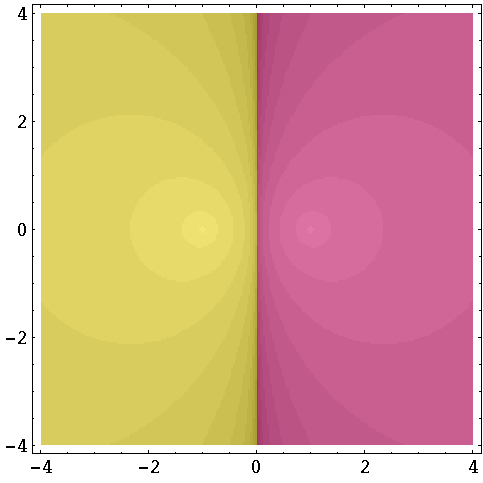
\includegraphics[width=0.5\textwidth]{NDfigura0.pdf}
\caption{Cuencas de atracción de las raíces, $z=-1$ y  $z=1$ para el método de Newton aplicado al polinomio $p(z)=(z-1)^2(z+1)$.}
\label{fig4:41}
\end{figure}

 En primer lugar, mediante cambios de variable afines, el estudio del método de Newton aplicado a polinomios de la forma (\ref{eq5}), puede reducirse al estudio del polinomio $p(z)=(z-1)^2(z+1)$. En este caso, la función de iteración del método de Newton es de la forma
 $$
 N_p(z)=\frac{2z^2+z+1}{1+3z}.
 $$
 Esta función tiene un punto fijo superatractor en $z=-1$ y un punto fijo atractor en $z=1$, con multiplicador asociado $1/2$. Además, el punto del infinito es un punto fijo repulsor con multiplicador asociado $3/2$. En la figura~\ref{fig4:41} se muestran las cuencas de atracción de las dos raíces, $z=-1$ y  $z=1$. Como se puede apreciar en la figura, la cuenca de atracción de la raíz múltiple, en este caso, $z=1$, <<invade>> la cuenca de atracción de la otra raíz, $z=-1$.  En este caso, la presencia  de dos raíces, una múltiple y otra simple,  hace que se pierda la simetría a la que hace referencia el teorema~\ref{Teorema444}.

Por otra parte, para el caso de polinomios con raíces múltiples de la forma (\ref{eq5}) la iteración de Newton, $N_p(z)$, es conjugada mediante la transformada de M\"obius $M(z)=(z-a)/(z-b)$ con la aplicación $z(z+1)/2$ definida en el plano complejo ampliado $\hat \C$. El correspondiente conjunto de Julia  se muestra en la figura~\ref{figura1230}.
\begin{figure}[htbp]
    \centering
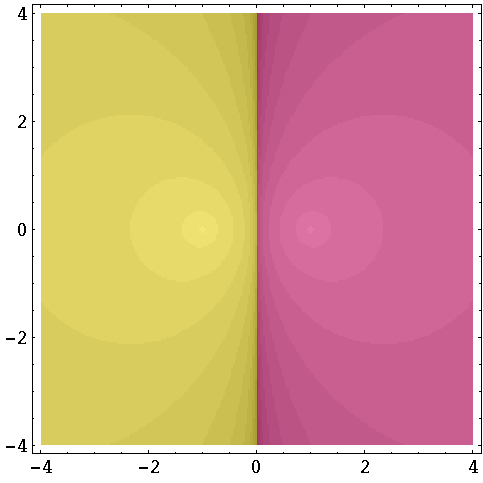
\includegraphics[width=0.45\textwidth]{NDfigura0.pdf}
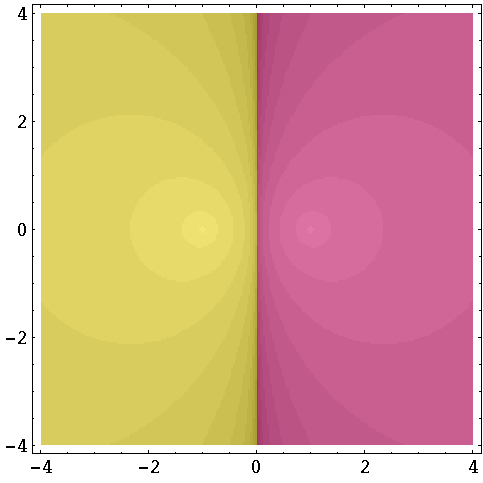
\includegraphics[width=0.45\textwidth]{NDfigura0.pdf}
    \caption{Cuencas de atraccción asociadas a las funciones de iteración  $z(z+1)/2$ y $z^2-3/4$, relacionadas respectivamente con el método de Newton y el método de Newton para raíces múltiples.}
    \label{figura1230}
 \end{figure}
 
Si se conoce la multiplicidad $m$ de la raíz a aproximar,  el conocido como método de Newton para raíces múltiples,
\begin{equation}\label{NwMul}
N_m(z)=z-m\frac{p(z)}{p'(z)}
\end{equation}
tiene la ventaja de que recupera el orden de convergencia cuadrático al aproximar la raíz múltiple. El estudio de la dinámica del método~(\ref{NwMul})
para  polinomios de la forma (\ref{eq5}) lo realizó Gilbert \cite{Gilbert}. En ese trabajo, se prueba que la correspondiente función de iteración para polinomios de la forma (\ref{eq5}) es
\begin{equation}\label{NwMul7}
N_2(z)=z-2\frac{p(z)}{p'(z)}=\frac{z^2+az-2ab}{3z-a-2b}.
\end{equation}
Esta función racional  es conjugada con la aplicación $z^2-3/4$ mediante la transformada de M\"obius 
$$
M(z)=\frac{3z+a-4b}{2(z-a)}.
$$ 
El comportamiento dinámico de la función polinómica $z^2-3/4$ es bien conocido (véase \cite{Beardon}, por ejemplo). En el segundo gráfico de la figura~\ref{figura1230} se muestra el conjunto de Julia  para $z^2-3/4$, que es la frontera de la región de negro. Nótese que en este caso, las raíces $a$ y $b$ del polinomio (\ref{eq5}) se transforman por $M$ en los puntos
$$
M(a)=\infty, \quad M(b)=-\frac{1}{2}.
$$
Estos dos puntos $\infty$ y $-1/2$, junto con el punto $3/2$, son los puntos fijos del polinomio $z^2-3/4$. $\infty$ es un punto fijo superatractor, $-1/2$ es un punto fijo indiferente y $3/2$ es un punto fijo repulsor. Deshaciendo los cambios se concluye que el método de Newton para raíces múltiples (\ref{NwMul7}) ha transformado la raíz múltiple $a$ en un punto fijo superatractor. Como contrapartida, la otra raíz, $b$, pasa a ser un punto fijo indiferente. Por último $\infty$ es un punto fijo repulsor para~(\ref{NwMul7}).

El segundo gráfico de la figura~\ref{figura1230}  muestra la cuenca de atracción de $\infty$ como punto fijo de $z^2-3/4$. Los puntos de la región de negro convergen al punto fijo indiferente $-1/2$, aunque, en este caso la convergencia es extremadamente lenta.

Otra variante del método de Newton para ecuaciones con raíces múltiples viene dada por
\begin{equation}\label{NwMul2}
\hat{N}_p(z)=z-\frac{1}{1-L_p(z)}\frac{p(z)}{p'(z)}, \quad L_p(z)=\frac{p(z)p''(z)}{p'(z)^2}.
\end{equation}
$\hat{N}_p(z)$ se obtiene aplicando el método de Newton a la función racional $p(z)/p'(z)$. Para polinomios de la forma (\ref{eq5}), el método~\ref{NwMul2}
 es conjugado con la aplicación $-z^2$ mediante la transformada de Möbius $M(z)=(z-a)/(z-b)$. Por lo tanto, su conjunto de Julia  es la circunferencia unidad y sus dinámicas son similares al método de Newton para raíces simples (véase el teorema~\ref{Teorema444}).



\subsection{El método de Newton para polinomios cúbicos}
\index{Newton, I.!método}

Sea $p(z)= a_3z^3+a_2z^2+a_1z+a_0$  un polinomio cúbico con
sus tres raíces  $a$, $b$ y $c$ distintas, las
cuales suponemos ordenadas por sus módulos, es decir,  $0 \le
|a| \le |b| \le |c|$.

Pongamos $ T^{-1}(z) = \alpha z + \beta $, y encontremos los
coeficientes $ \alpha$ y $ \beta$  de modo que $
T^{-1}(a) = 0$ y $ T^{-1}(c) = 1$. Tenemos entonces que $
\alpha = \frac{1}{c-a}$ y $ \beta = - \frac{a}{c-a}$, por lo
tanto, $ T^{-1}(z) = \frac{z}{c-a} - \frac{a}{c-a}$, y en
consecuencia $ T(z) = (c-a) z + a$. Aplicando esta
transformación $T$ en el teorema de  reescalamiento\index{reescalamiento}
anterior (teorema~\ref{reescalamiento}), obtenemos
$$
q(z) = p \circ T (z)  = p ( (c-a) z + a)= (c-a)^3 z \left( z -
\frac{b-a}{c-a}\right) ( z -1 ) .
$$
Haciendo, $ \lambda = ( c - a)^3$ y $ \rho =
(b-a)/(c-a)$, obtenemos
$$
q(z) = \lambda^3  z ( z - 1)( z - \rho ) .
$$

Por otra parte, es fácil ver que si $ f(z) = \alpha g(z)$,
entonces  $ N_f(z) =
N_g(z)$.

En consecuencia,  haciendo 
\begin{equation}\label{prho}
p_{\rho}(z) = z (z-1)(z-\rho)
\end{equation}
 y
denotando por $N_{\rho}$ a su correspondiente función de iteración para el método de Newton,
\begin{equation}\label{Nro}
 N_{\rho}(z)=z-\frac{ z (z-1)(z-\rho)}{3 z^2-2 \rho z-2 z+\rho},
\end{equation}
 tenemos
probado el siguiente resultado, que establece que para conocer la
di\-ná\-mi\-ca de la método de Newton de un polinomio
cúbico debemos conocer la dinámica de la función racional $N_{\rho}$, donde $ \rho \in \C$ es un parámetro.

\begin{teorema}
Sea $ p(z)$ un polinomio cúbico con sus tres raíces
distintas. Entonces, $ N_p$ es conjugado topológicamente con
$N_{\rho}$ definida en~(\ref{Nro}).
\end{teorema}

Notemos que el caso $ \rho = 0 $ se reduce al estudio del método de Newton aplicado al polinomio $ p_0 (z) = z^2 (z-1) = z^3 -
z^2$. Este polinomio tiene en $0$ una raíz doble y su comportamiento dinámico es similar al del polinomio que aparece en la figura~\ref{fig4:41}.

En este caso, tenemos
$$
N_{\rho} (z) =  z -
 \frac{z^3 - (\rho + 1) z^2 + \rho z}{ 3 z^2 - 2 (\rho + 1 )z + \rho}
= \frac{2 z^3 - (\rho + 1 ) z^2}{ 3 z^2 - 2 (\rho + 1) z + \rho}
$$
y
$$
N_{\rho}'(z) = \frac{( z^3 - (\rho +1 )z^2 + \rho z) ( 6 z - 2
(\rho +1)}{ (3 z^2 - 2 (\rho + 1) z + \rho )^2}.
$$
Un estudio sobre de familia fue hecho por Curry, Garnett  y
Sullivan  \cite{CGS}.


En este caso,  $ N_{\rho}'(z) = 0 $ si y sólo si $p_{\rho}
(z) = 0$  o $ p_{\rho}''(z) =
0$.  En consecuencia, el conjunto de puntos críticos de $ N_{\rho}$ está formado por  las tres raíces de $ p_{\rho}$ junto con el punto $ z = \frac{\rho +1 }{3}$. Los puntos
críticos de $N_{\rho}$ que no son raíces de $
p_{\rho}$ se llaman \emph{puntos críticos libres}.%
\index{punto crítico libre}

El estudio de las órbitas de los puntos críticos libres da mucha información sobre el comportamiento dinámico de un método. En concreto, para determinar si
existen órbitas periódicas atractoras para $N_{\rho}$,
distintas de las raíces de $ p_{\rho}$, debemos responder
a la pregunta siguiente: ¿para  qué valores de $\rho$, la órbita del punto crítico libre, 
$$
N_{\rho}^{n}\left(\frac{\rho+1}{3}\right)
$$ 
es una órbita periódica
atractora?



En la pregunta anterior debemos excluir los casos
 $ \rho = -1$, $ \rho = 2 $ y
$ \rho = 1/2$ para los cuales el punto fijo extraño coincide con alguna de las raíces del polinomio   $ p_{\rho}$.


Una manera de responder a la pregunta anterior es colorear el espacio de parámetros $\rho\in\C$ de acuerdo a la convergencia del punto crítico libre $(\rho+1)/3$, tal y como se hace en la figura~\ref{esparam_fig0}. Si la órbita de $(\rho+1)/3$ converge a 0, 1 o $\rho$, el valor del correspondiente parámetro $\rho$ se colorea en amarillo, cian o magenta respectivamente.

\begin{figure}[htb]
\centering
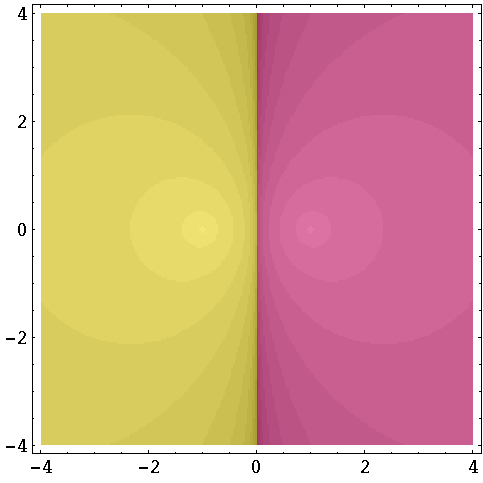
\includegraphics[width=0.45\textwidth]{NDfigura0.pdf}
\qquad
 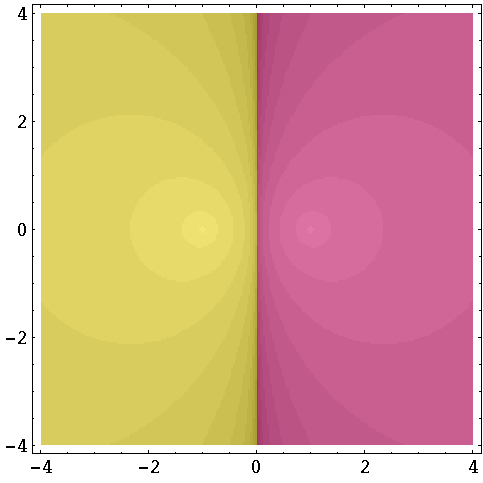
\includegraphics[width=0.45\textwidth]{NDfigura0.pdf}
 %\vspace{-1.25cm}
\caption{Representación gráfica del espacio de parámetros asociado a la función de iteración $N_{\rho}(z)$ definida en~(\ref{Nro}) y asociada a los polinomios de la forma $p_{\rho}(z) = z (z-1)(z-\rho)$. La figura de la derecha muestra una ampliación de una zona negra en la que se aprecia  un conjunto de tipo Mandelbrot.}
 \label{esparam_fig0}
\end{figure}


Como se aprecia en la figura~\ref{esparam_fig0}, existen regiones abiertas en el \emph{espacio de parámetros} tales que, si $\rho$ pertenece a estas regiones entonces existen regiones abiertas en el plano complejo de forma que 
$N_{\rho}(z)$ definida en~(\ref{Nro}) no converge a ninguna de las raíces del polinomio $p_{\rho}(z)$ definido en~(\ref{prho}). Las regiones coloreadas en negro en el espacio de parámetros están formadas por los valores de $\rho$ para los cuales la sucesión
$$
N_{\rho}^{n}\left(\frac{\rho+1}{3}\right)
$$ 
va a parar a  un ciclo atractor.

La parametrización de los polinomios cúbicos considerada en (\ref{prho}) no es la única. Otra parametrización muy habitual (véase \cite{Roberts}) es la siguiente:
\begin{equation}\label{pnu}
p_{\mu}(z)=(z^2-1)(z-\mu), \quad \mu\in\C.
\end{equation}
La correspondiente función de iteración para el método de Newton es
\begin{equation}\label{Nnu}
 N_{\mu}(z)=\frac{ 2z^3-\mu z^2-\mu}{3 z^2-2 \mu z-1}.
\end{equation}

En este caso, el punto crítico libre asociado al método de Newton es la única raíz de $p''_{\mu}(z)=0$, es decir, $z=\mu/3$. Podemos realizar una reflexiones similares al caso anterior y colorear el espacio de parámetros conforme a la convergencia del punto crítico libre, amarillo, cian o magenta si la órbita de $\mu/3$ converge a 
$\mu$, 1 o $-1$ respectivamente, tal y como se muestra en la figura~\ref{esparam_fig1}.  De nuevo, las regiones coloreadas en negro en el espacio de parámetros están formadas por los valores de $\mu$ para los cuales la sucesión
$$
N_{\mu}^{n}\left(\frac{\mu}{3}\right)
$$ 
va a parar a  un ciclo atractor.

\begin{figure}[htb]
\centering
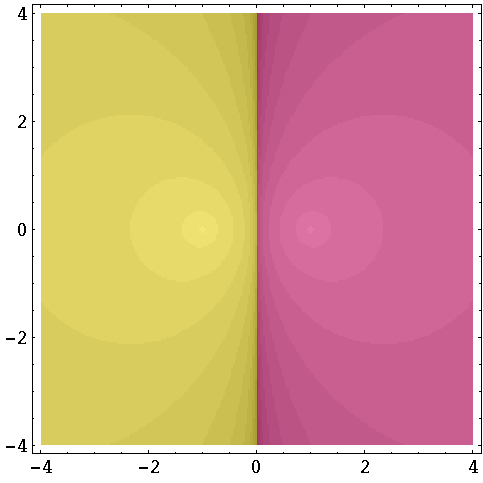
\includegraphics[width=0.45\textwidth]{NDfigura0.pdf}
\qquad
 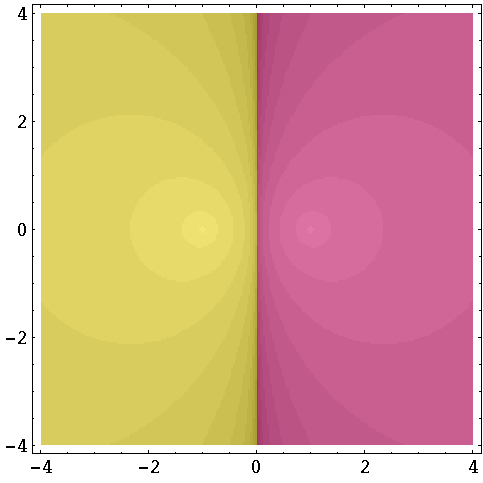
\includegraphics[width=0.45\textwidth]{NDfigura0.pdf}
 %\vspace{-1.25cm}
\caption{Representación gráfica del espacio de parámetros asociado a la función de iteración del método de Newton para los polinomios~(\ref{pnu}). La figura de la derecha muestra una ampliación de una zona negra en la que se aprecia un conjunto de tipo Mandelbrot similar al de la figura~\ref{esparam_fig0}.}\index{Mandelbrot, B.!conjunto}
\label{esparam_fig1}
\end{figure}




Por último, consideramos  otra parametrización muy conocida (véase \cite{PlazaRomero}), como es la siguiente:
\begin{equation}\label{plambda}
p_{\lambda}(z)=z^3+(\lambda-1)z-\lambda, \quad \lambda\in\C.
\end{equation}
Denotamos $N_{\lambda}(z)$ a la función de iteración del método de Newton aplicado a los polinomios de la forma~(\ref{plambda}):
\begin{equation}\label{Nlambda}
N_{\lambda}(z)=\frac{2z^3+\lambda}{3z^2+\lambda-1}.
\end{equation}
\index{espacio de parámetros}%
En este caso, el punto crítico libre asociado al método de Newton es la única raíz de $p''_{\lambda}(z)=0$, es decir, $z=0$. 

Las regiones coloreadas en negro en el espacio de parámetros de la  figura~\ref{esparam_fig2} están formadas por los valores de $\lambda$ para los cuales la sucesión
$$
N_{\lambda}^{n}(0)
$$ 
va a parar a  un ciclo atractor.

\begin{figure}[htb]
\centering
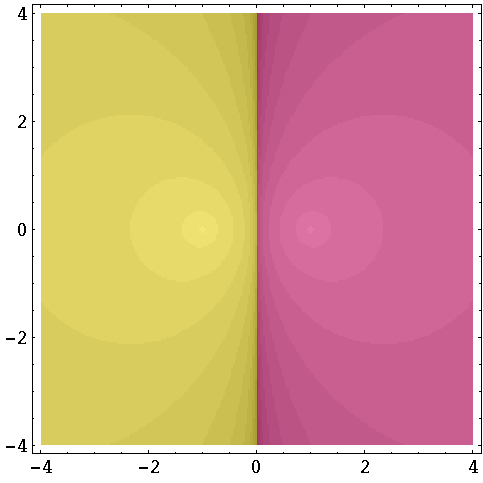
\includegraphics[width=0.45\textwidth]{NDfigura0.pdf}
\qquad
 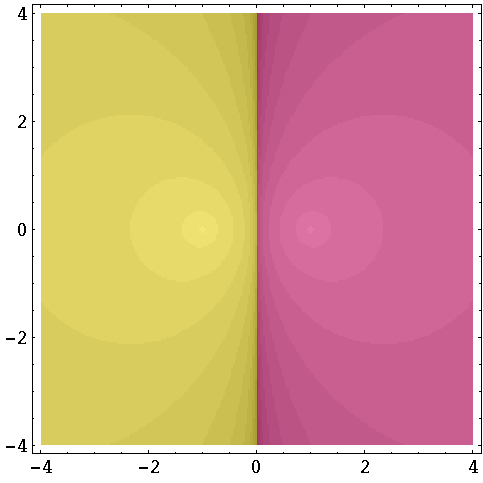
\includegraphics[width=0.45\textwidth]{NDfigura0.pdf}
 %\vspace{-1.25cm}
\caption{Representación gráfica del espacio de parámetros asociado a la función de iteración $N_{\lambda}(z)$ definida en~(\ref{Nlambda}) y la correspondiente ampliación mostrando un conjunto de tipo Mandelbrot.}\index{Mandelbrot, B.!conjunto}
 \label{esparam_fig2}
\end{figure}


La figura~\ref{esparam_fig3} muestra las cuencas de atracción del método de Newton para un polinomio $p_{\lambda}(z)$ definido en~(\ref{plambda}) y tomando $\lambda$ en una de las zonas negras del espacio de parámetros. Como vemos aparecen <<agujeros negros>> originados por la presencia de ciclos atractores. En concreto, en este caso se tiene que la órbita del punto crítico libre $z=0$ es atraída por el 3-ciclo
$$
\{1.02169 - 1.04136i, 0.620968  - 0.632698 i, -0.00204529 + 
 0.00527748 i \}.
$$

\begin{figure}[htb]
\centering
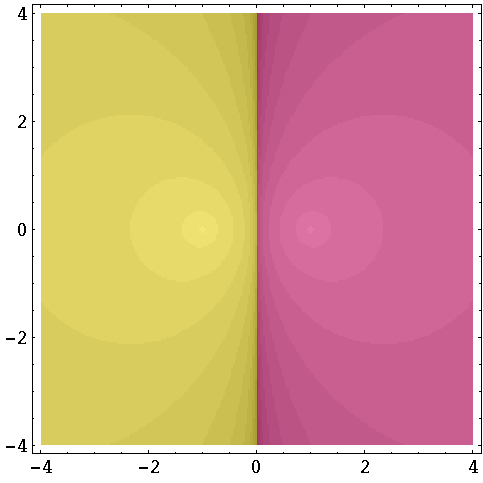
\includegraphics[width=0.45\textwidth]{NDfigura0.pdf}
\qquad
 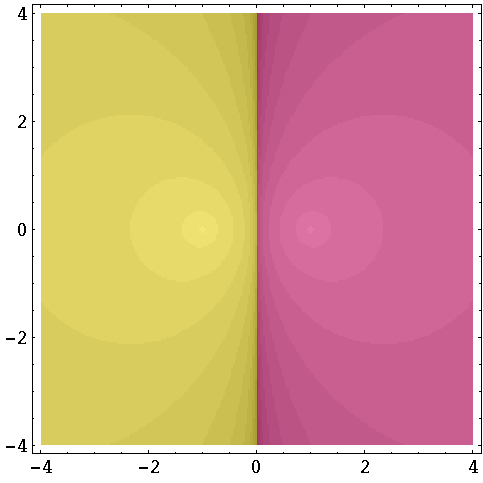
\includegraphics[width=0.45\textwidth]{NDfigura0.pdf}
 %\vspace{-1.25cm}
\caption{Cuencas de atracción del método de Newton aplicado al  polinomio $p_{\lambda}(z)=z^3+(\lambda-1)z-\lambda$ con $\lambda=1.02+0.96i$ y una ampliación de la zona negra que se genera entorno al punto crítico libre $z=0$.}
 \label{esparam_fig3}
\end{figure}


\subsection{El método de Newton para polinomios de grados 4 y 5} 
\index{Newton, I.!método}

Como hemos visto en el apartado anterior, el estudio dinámico del método de Newton aplicado a polinomios de tercer grado se reduce al estudio de una función racional dependiente de un parámetro, en concreto~(\ref{Nro}). Evidentemente, al aumentar el grado de los polinomios también lo hará el número de parámetros involucrados en la correspondiente función racional asociada al método de Newton.

No obstante, existen algunas manipulaciones algebraicas que permiten reducir el número de coeficientes que aparecen en una ecuación polinómica. En concreto, la conocida como \emph{transformación de Tschirnhaus} (\cite{Dickson}) permite transformar la ecuación\index{transformación de Tschirnhaus}
$$
z^n+a_{n-1}z^{n-1}+\cdots+a_{1}z+a_0=0, \quad n>2,
$$
en otra ecuación polinómica donde no aparecen los términos en $z^{n-1}$ y $z^{n-2}$, es decir,
$$
z^n+b_{n-3}z^{n-3}+\cdots+b_{1}z+b_0=0, \quad n>2.
$$
El resultado original de Tschirnhaus apareció publicado en \emph{Acta Eruditorum} en 1683. Más adelante, en 1786, E. S. Bring probó que una ecuación polinómica de grado 5 puede reducirse a una del tipo
$$
z^5+az+b=0.
$$
Finalmente, en 1834 G. B. Jerrard demostró que en ecuaciones polinómicas de grado mayor que 3 se puede encontrar  una transformación de Tschirnhaus en la que no aparecen los términos en $z^{n-1}$, $z^{n-2}$ y $z^{n-3}$, es decir, del tipo
$$
z^n+c_{n-4}z^{n-4}+\cdots+c_{1}z+c_0=0, \quad n>3.
$$

Estas transformaciones se basan en complicadas manipulaciones algebraicas sobre las raíces de la ecuación (véase \cite{WeissBJ}). Estas manipulaciones no conservan las propiedades dinámicas. En efecto, como se vio en el ejemplo~(\ref{ejem4.5}), el  método de Newton aplicado al polinomio $z^3-2z+2$ tiene un 2-ciclo atractor de la forma $\{0,1\}$. Dicho polinomio puede ser transformado en uno de la forma $p(z)=z^3-\lambda^3$, $\lambda\in \C$, por la correspondiente transformación de Tschirnhaus. A su vez, el método de Newton aplicado al polinomio anterior,
$$
N_p(z)=z-\frac{z^3-\lambda^3}{3z^2}=\frac{2z^3+\lambda^3}{3z^2}
$$
 es conjugado topológicamente, mediante la aplicación afín $h(z)=z/\lambda$, con el método de Newton aplicado al polinomio $q(z)=z^3-1$,
$$
N_q(z)=z-\frac{z^3-1}{3z^2}=\frac{2z^3+1}{3z^2}.
$$
En efecto,
$$
h\circ N_p(z)=\frac{2z^3+\lambda^3}{3\lambda z^2}=N_q\circ h(z).
$$
Pero como se aprecia en las figuras~\ref{C4fig:1} y~\ref{fig44:2}, el comportamiento dinámico del método de Newton aplicado a los polinomios $q(z)=z^3-1$ y $z^3-2z+2$ es muy diferente. De hecho, en el primer caso no aparecen $n$-ciclos atractores con $n\ge 2$, luego su dinámica no puede ser equivalente a la del método de Newton aplicado al polinomio $z^3-2z+2$, que sí presenta un 2-ciclo atractor.

Para ver que $N_p(z)$ no tiene 2-ciclos atractores, calculamos los puntos fijos de 
$$
N_p^2(z)=\frac{16 z^9+51 z^6+12z^3+2}{9 z^2 \left(2  z^3+1\right)^2}.
$$
Tenemos que $N_p^2(z)=z$ si y sólo si $z^3=1$ o $20 z^6+5 z^3+2=0$. Los 2-ciclos aparecen entre las raíces $\xi_j$, $j=1,\dots, 6$ de la segunda ecuación. Pero en todas ellas se cumple que 
$$
|N'_p(\xi_j)|\approx 2.45>1,
$$
luego ningún 2-ciclo es atractor.

Las expresiones simplificadas de polinomios de cuarto y quinto grado que aparecen después de aplicar las transformaciones de Tschirnhaus o de Bring-Jerrard, motivan el estudio del método de Newton para ecuaciones de la forma $z^4+az+b^4=0$ o $z^5+az+b^5=0$ como casos particulares de ecuaciones polinómicas de cuarto y quinto grado respectivamente. En concreto, para la ecuación de quinto grado anterior puede verse un estudio detallado de la dinámica del método de Newton en~\cite{Balibrea}.












%% !TEX root = MemoriaVGalilea.tex
% !TEX encoding = UTF-8 Unicode
% !TEX TS-program = pdflatex
% !TEX spellcheck = Spanish
%
%%%%%%%%%%%%%%%%%%%%%%%%%%
%----- VERSION: 9-10-2025
%%%%%%%%%%%%%%%%%%%%%%%%%%

\chapter[Capítulo de prueba]{Capítulo de prueba} 
\label{capituloPRUEBA}


Esto es solo un ejemplo para ver cómo quedaría un capítulo nuevo, que habría que incluir con la orden include de \LaTeX
%CAPITULO 4
% \chapter{Estudio dinámico de los métodos de Schröder, Halley y Chebyshev en el plano complejo}


% Resumir lo hecho en el TFM.

% 4.1. Definición general y propiedades de cada método
% 4.2. Análisis de las funciones racionales asociadas
% 4.3. Estudio de los conjuntos de Julia y Fatou
% 4.4. Análisis del plano de parámetros
% 4.5. Comparación con el método de Newton en términos dinámicos
% 4.6. Comparación con el método de Newton en términos numéricos

% % TesisVG_Cap5.tex
% Capítulo 5: Estudio dinámico en la recta real
\chapter{Estudio dinámico de los métodos de Schröder, Halley y Chebyshev en el plano complejo}
\label{cap:plano_complejo}

% Resumir lo hecho en el TFM.

% \subsection{Construcci\'on del m\'etodo de Chebyshev}
% Sea $f:\mathbb{R}\to\mathbb{R}$ de clase $\mathcal{C}^3$ en un entorno de una ra\'iz simple $\alpha$ tal que $f(\alpha)=0$ y $f'(\alpha)\neq 0$. Denotamos el error $e_n=x_n-\alpha$. La idea es partir del paso de Newton y a\~nadir una correcci\'on cuadr\'atica que elimine el t\'ermino dominante del error para obtener convergencia de orden tres.

% Usando el desarrollo de Taylor de $f$ y sus derivadas alrededor de $\alpha$, escribimos
% \[
% f(x)=f'(\alpha)e+\tfrac{1}{2}f''(\alpha)e^2+\tfrac{1}{6}f^{(3)}(\alpha)e^3+\mathcal{O}(e^4),\qquad
% f'(x)=f'(\alpha)+f''(\alpha)e+\tfrac{1}{2}f^{(3)}(\alpha)e^2+\mathcal{O}(e^3),
% \]
% con $e=x-\alpha$. Si definimos
% \[
% t(x)=\frac{f(x)}{f'(x)},
% \]
% entonces una expansi\'on formal da
% \[
% t(x)=e-c_2e^2+\bigl(2c_2^2-c_3\bigr)e^3+\mathcal{O}(e^4),\quad c_2=\frac{f''(\alpha)}{2f'(\alpha)},\; c_3=\frac{f^{(3)}(\alpha)}{6f'(\alpha)}.
% \]
% El paso de Newton $x- t(x)$ produce un error $e_{n+1}=c_2e_n^2+\mathcal{O}(e_n^3)$. Para anular el t\'ermino cuadr\'atico, consideramos una correcci\'on de la forma $x- t(x)-b(x)\,t(x)^2$ y escogemos
% \[
% b(x)=\frac{1}{2}\,\frac{f''(x)}{f'(x)}.
% \]
% Con esta elecci\'on, el nuevo iterador reduce el error a orden c\'ubico, con ecuaci\'on de error
% \[
% e_{n+1}=c_3\,e_n^3+\mathcal{O}(e_n^4)=\frac{f^{(3)}(\alpha)}{6f'(\alpha)}\,e_n^3+\mathcal{O}(e_n^4).
% \]

% En forma cerrada, el \textit{m\'etodo de Chebyshev} queda
% \begin{equation}
% \label{eq:chebyshev}
%  x_{n+1} 
% 	= x_n 
% 	- \frac{f(x_n)}{f'(x_n)} 
% 	- \frac{1}{2}\,\frac{f''(x_n)}{f'(x_n)}\left(\frac{f(x_n)}{f'(x_n)}\right)^{\!2}.
% \end{equation}
% Este esquema tiene orden de convergencia tres bajo las condiciones indicadas y constante asint\'otica $\left|\tfrac{f^{(3)}(\alpha)}{6f'(\alpha)}\right|$. En comparaci\'on con Halley, requiere una evaluaci\'on adicional de $f''$, pero evita cocientes m\'as costosos como en Halley, siendo una alternativa de tercer orden basada en una correcci\'on sobre Newton que cancela el error cuadr\'atico.

% % Desarrollo ampliado basado en el PDF adjunto
% \subsubsection{Construcciones del m\'etodo de Chebyshev}

El m\'etodo de Chebyshev es un esquema iterativo de tercer orden para la
aproximaci\'on de ra\'{\i}ces simples de ecuaciones no lineales $f(x)=0$.
Su expresi\'on cl\'asica, partiendo de un $x_n$ suficientemente pr\'oximo a la ra\'{\i}z
$\alpha$, es
\begin{equation}
\label{eq:chebyshev-clasico}
 x_{n+1} 
 	= x_n 
 	- \frac{f(x_n)}{f'(x_n)} 
 	- \frac{1}{2}\,\frac{f''(x_n)}{f'(x_n)}\left(\frac{f(x_n)}{f'(x_n)}\right)^{\!2}.
\end{equation}
Este m\'etodo, junto con sus mejoras y variantes, ha sido estudiado extensamente
en la literatura debido a su buena eficiencia y a que puede deducirse de varias
maneras equivalentes.

\paragraph{Interpolaci\'on cuadr\'atica inversa.}
Una primera construcci\'on procede de aproximar la inversa local $g=f^{-1}$
en torno a $y=0$ mediante interpolaci\'on cuadr\'atica u osculadora.
Al imponer condiciones de Hermite adecuadas en $y=f(x_n)$ (valores y derivadas
que dependen de $1/f'(x_n)$ y $-f''(x_n)/f'(x_n)^3$), y evaluar en $y=0$, se
obtiene precisamente la actualizaci\'on \eqref{eq:chebyshev-clasico}.

\paragraph{Par\'abola tangente.}
Otra deducci\'on geom\'etrica recurre a una par\'abola osculadora a la gr\'afica de $f$.
Consideremos la familia
\begin{equation}
\label{eq:parabola-osculadora}
 a\,\bigl(y-f(x_n)\bigr)^2 + \bigl(y-f(x_n)\bigr) + b\,(x-x_n) = 0,
\end{equation}
cuya gr\'afica $y=y(x)$ satisface condiciones de tangencia en $x_n$:
$y(x_n)=f(x_n)$, $y'(x_n)=f'(x_n)$, $y''(x_n)=f''(x_n)$. Derivando
\eqref{eq:parabola-osculadora} y evaluando en $(x_n,f(x_n))$ se obtiene
$b=-y'(x_n)=-f'(x_n)$. Una segunda derivada y evaluaci\'on conduce a
\[ a=-\,\frac{y''(x_n)}{2\,y'(x_n)^2}=-\,\frac{f''(x_n)}{2\,f'(x_n)^2}. \]
Imponiendo $y=0$ (intersecci\'on con el eje $OX$) en \eqref{eq:parabola-osculadora}
y despejando $x$, resulta
\[
 x_{n+1}=x_n-\frac{f(x_n)}{f'(x_n)}-\frac{1}{2}\,\frac{f''(x_n)}{f'(x_n)}\left(\frac{f(x_n)}{f'(x_n)}\right)^{\!2},
\]
que coincide con \eqref{eq:chebyshev-clasico}.

\paragraph{Interpolaci\'on exponencial.}
Una tercera v\'ia de construcci\'on utiliza una curva aproximante de la forma
\begin{equation}
\label{eq:interpolacion-exp}
 y(x) = e^{a(x-x_n)}\,\bigl(b\,(x-x_n)+c\bigr),
\end{equation}
con par\'ametros $a,b,c$ escogidos para satisfacer condiciones de osculaci\'on en $x_n$:
$y(x_n)=f(x_n)$, $y'(x_n)=f'(x_n)$ y $y''(x_n)=f''(x_n)$. De la primera condici\'on
se deduce $c=f(x_n)$ y de la segunda $b=f'(x_n)-a\,f(x_n)$. La tercera condici\'on
impone la relaci\'on $2a\,f'(x_n)-a^2 f(x_n)=f''(x_n)$. Al intersectar \eqref{eq:interpolacion-exp}
con $y=0$ (esto es, imponiendo $b\,(x-x_n)+c=0$) se obtiene la actualizaci\'on
\[
 x_{n+1}=x_n-\frac{c}{b}=x_n-\frac{f(x_n)}{f'(x_n)-a\,f(x_n)}.
\]
La elecci\'on de $a$ que anula el t\'ermino cuadr\'atico del error (esto es, que asegura
convergencia c\'ubica) conduce de nuevo a la forma \eqref{eq:chebyshev-clasico}.

\medskip
Estas construcciones muestran que el m\'etodo de Chebyshev puede interpretarse
como una correcci\'on de Newton que cancela el t\'ermino de error de segundo orden
por medio de informaci\'on de segunda derivada. Bajo supuestos habituales
($f\in\mathcal{C}^3$, $f'(\alpha)\neq0$ y $x_n$ cercano a $\alpha$), el m\'etodo es de
orden tres y su ecuaci\'on de error local es
\[
 e_{n+1}=\frac{f^{(3)}(\alpha)}{6f'(\alpha)}\,e_n^3+\mathcal{O}(e_n^4).
\]



\section{Definición general y propiedades de cada método}
Los tres métodos iterativos de orden tres que se estudiarán en este capítulo son el método de Schröder, el método de Halley y el método de Chebyshev. Cada uno de ellos puede definirse mediante una función racional asociada a una función meromorfa \( f:\mathbb{C}\to\mathbb{C} \). A continuación, se presentan las definiciones y propiedades fundamentales de cada método. y los
expresarames en función del operador:
\[
 L_f(x)=\frac{f(x)f''(x)}{(f'(x))^2}.
\]
\subsection{Definición y propiedades del método de Schröder}

Sea $f:\mathbb{C}\to\mathbb{C}$ una función meromorfa. El método de Schröder asociado a $f$ es el método iterativo definido por la función racional:
\begin{equation}
	S_f(z) = z - \frac{1}{1-L_f'(z)} 
    	\frac{f(z)}{f'(z)}
\end{equation}



\subsection{Definición y propiedades del método de Halley}

Sea $f:\mathbb{C}\to\mathbb{C}$ una función meromorfa. El método de Halley asociado a $f$ es el método iterativo definido por la función racional:
\begin{equation}
	H_f(z) = z - \frac{1}{1-\frac{L_f'(z)}{2}} 
    	\frac{f(z)}{f'(z)}
\end{equation}




\subsection{Definición y propiedades del método de Chebyshev}
Sea $f:\mathbb{C}\to\mathbb{C}$ una función meromorfa. El método de Chebyshev asociado a $f$ es el método iterativo definido por la función racional:
\begin{equation}
	C_f(z) = z - \frac{f(z)}{f'(z)} \left( 1+\frac{L_f(z)}{2}\right),
\end{equation}

\section{Análisis de las funciones racionales asociadas}
\section{Estudio de los conjuntos de Julia y Fatou}
\section{Análisis del plano de parámetros}
\section{Comparación con el método de Newton en términos dinámicos}
\section{Comparación con el método de Newton en términos numéricos}


%\section{Dinámica del método de Schr\"oder en el plano complejo}
%
%\subsection{Polinomios con dos raíces}
%
%Resumir lo hecho en el artículo \cite{Galilea21}
%
%\subsection{Polinomios de grado tres}
%
%Esto es lo que debemos desarrollara ahora
%\subsection{Polinomios de grado tres: comportamiento del punto del infinito.
%}
%%\item En el plano complejo ampliado $\hat{\mathbb{C}}= \mathbb{C}\cup \{\infty\}$, el $\infty$ puede interpretarse como un punto más del plano complejo. 
%%\item Método de Newton \cite{Traub}: $\infty$ único punto fijo extraño (repulsor).
%%\item Método de Schröder: $\infty$ no es siempre un punto fijo.
%%\item Tiene sentido estudiar sus órbitas para distintas familias de funciones: ¿a dónde va a parar el punto del infinito por le método de  Schröder?
%%\item El comportamiento de $\infty$ para $S_p(z)$ es el mismo que el comportamiento de $0$ para
%%\begin{equation}\label{eq2}
%%T_{p}(z)=\frac{1}{S_{p}(1/z)}
%
%\section{Dinámica del método de Schr\"oder en la recta real}

%CAPITULO 5
% TesisVG_Cap5.tex
% Capítulo 5: Método de Schröder en el plano complejo
\chapter{Método de Schröder en el plano complejo}
\label{cap:schroder_plano_complejo}

En este capítulo presentamos un estudio completo de la dinámica del método de Schröder en el plano complejo. Comenzamos introduciendo el método y sus propiedades fundamentales, para después analizar su comportamiento aplicado a polinomios con dos raíces de multiplicidades arbitrarias y, finalmente, extender el estudio a polinomios cúbicos mediante el análisis del plano de parámetros. Los resultados teóricos se ilustran mediante diagramas de cuencas de atracción que revelan la estructura fractal subyacente.

\section{Introducción: Método de Schröder y conceptos fundamentales}

\subsection{Definición del método de Schröder}

El método de Schröder fue introducido por Ernst Schröder en su trabajo seminal de 1870 \cite{Sch} sobre la resolución de ecuaciones no lineales. Schröder construyó este método aplicando el método de Newton a la ecuación $\tfrac{f(z)}{f'(z)}=0$, obteniendo el esquema iterativo
\begin{equation}
 z_{k+1}=S_f(z_k)=z_k-\frac{f(z_k)f'(z_k)}{f'(z_k)^2-f(z_k)f''(z_k)}, \quad k\ge 0, \quad z_0\in\C.
 \label{eq:Sch_def}
\end{equation}
Una ventaja importante del método de Schröder, señalada por el propio autor, es que converge cuadráticamente incluso para raíces múltiples, a diferencia del método de Newton que reduce su orden de convergencia en presencia de multiplicidad.

Para mayor comodidad, podemos escribir el iterador de Schröder en términos de la función
\begin{equation}
 L_f(z)=\frac{f(z)f''(z)}{\big(f'(z)\big)^2}
 \label{eq:Lf_def}
\end{equation}
como
\begin{equation}
 S_f(z)=z-\frac{1}{1-L_f(z)}\,\frac{f(z)}{f'(z)}.
 \label{eq:Sch_real}
\end{equation}

\subsection{Propiedades del método de Schröder}

Una ventaja importante del método de Schröder, señalada por el propio autor, es que converge cuadráticamente incluso para raíces múltiples, a diferencia del método de Newton que reduce su orden de convergencia en presencia de multiplicidad. Esto hace al método de Schröder particularmente valioso en situaciones donde se sospecha la existencia de raíces múltiples.

El coste computacional del método de Schröder es superior al de Newton: requiere evaluar no solo $f$ y $f'$, sino también $f''$, lo que lo sitúa en un nivel de coste comparable a los métodos de la familia Chebyshev-Halley.

\subsection{Conjugación topológica}

Una herramienta fundamental en el análisis de sistemas dinámicos es la conjugación topológica. Dos funciones $f,g: \C \to \C$ se dicen \emph{topológicamente conjugadas} si existe un homeomorfismo $\varphi$ tal que
$$
\varphi\circ g=f\circ \varphi.
$$
La conjugación topológica es muy útil porque funciones conjugadas comparten las mismas propiedades dinámicas desde el punto de vista topológico: los puntos fijos de una función se mapean en puntos fijos de la otra, los puntos periódicos corresponden entre sí, y lo mismo ocurre con las cuencas de atracción y los conjuntos de Julia.

\subsection{El problema de Cayley para polinomios cuadráticos}

En 1879, Arthur Cayley \cite{Cay} abordó el problema de caracterizar las cuencas de atracción del método de Newton aplicado a polinomios cuadráticos con raíces simples. Este problema, conocido como el \emph{problema de Cayley}, estableció las bases para el estudio de la dinámica compleja de métodos iterativos.

Cayley demostró que para el polinomio
\begin{equation}
f(z)=(z-a)(z-b),\quad a,b\in \C, \quad a\ne b,
\label{eq:poly_simple}
\end{equation}
la función iterativa de Newton es conjugada con la función $R(z)=z^2$ mediante una transformación de Möbius. El conjunto de Julia es la bisectriz entre las raíces $a$ y $b$, y las cuencas de atracción son los dos semiplanos correspondientes.

De manera análoga, el método de Schröder aplicado al mismo polinomio es conjugado con $-R(z)=-z^2$, produciendo el mismo conjunto de Julia y las mismas cuencas de atracción. Esto muestra que, para polinomios cuadráticos con raíces simples, ambos métodos tienen comportamiento dinámico idéntico.

\section{Polinomios con dos raíces de multiplicidades arbitrarias}

Consideramos ahora el caso más general de polinomios con dos raíces complejas de multiplicidades distintas:
\begin{equation}
 f(z)=(z-a)^m(z-b)^n,\qquad a,b\in\C,\ a\ne b,\quad m\ge n\ge 1.
 \label{eq:poly_dos_raices}
\end{equation}
Este caso es significativamente más interesante que el de raíces simples, pues la presencia de multiplicidades distintas rompe la simetría y produce conjuntos de Julia con geometría circular no trivial.

\subsection{Reducción al caso canónico mediante conjugación}

Para simplificar el análisis, realizamos una conjugación afín que traslada las raíces $a$ y $b$ a $1$ y $-1$ respectivamente. Definimos la transformación afín
\begin{equation}
A(z)=1+2\frac{z-a}{a-b}
\label{eq:afin}
\end{equation}
y consideramos la función conjugada
\begin{equation}
T_{m,n}(z)=A\circ S_f\circ A^{-1}(z)=\frac{(m-n) z^2 +2 (m+n) z +m-n}{(m+n) z^2 +2(m-n)z +m+n}.
\label{eq:Tmn}
\end{equation}
Esta función $T_{m,n}$ representa la dinámica del método de Schröder aplicado a $(z-1)^m(z+1)^n$ y depende únicamente de las multiplicidades $m$ y $n$.

Mediante una segunda conjugación con la transformación de Möbius
\begin{equation}
M(z)=\frac{z-1}{z+1}
\label{eq:Mobius}
\end{equation}
llegamos a una función racional extremadamente simple:
\begin{equation}
R_{m,n}(z)=M\circ T_{m,n}\circ M^{-1}(z)=-\frac{n}{m}z^2.
\label{eq:Rmn}
\end{equation}

\subsection{Análisis dinámico de $R_{m,n}$}

La función $R_{m,n}(z)=-\tfrac{n}{m}z^2$ tiene una dinámica completamente caracterizada. El círculo
$$
C_{m,n}=\left\{z\in\C; |z|=\frac{m}{n}\right\}
$$
es invariante bajo $R_{m,n}$. Los puntos con $|z_0|<m/n$ convergen al origen bajo iteración, mientras que los puntos con $|z_0|>m/n$ divergen a infinito. Por tanto, $C_{m,n}$ es el conjunto de Julia de $R_{m,n}$.

\section{Teoremas principales: caracterización del conjunto de Julia}

Los siguientes dos teoremas constituyen los resultados principales de este capítulo, caracterizando completamente el conjunto de Julia del método de Schröder para polinomios con dos raíces.

\begin{teorema}[Conjunto de Julia en el caso canónico]
\label{teo:julia_canonico}
Sea $T_{m,n}(z)$ la función racional definida por \eqref{eq:Tmn} y sea $J_{m,n}$ su conjunto de Julia. Entonces:
\begin{enumerate}
\item Si $m=n$, entonces $J_{m,m}$ es el eje imaginario.
\item Si $m>n\ge 1$, entonces $J_{m,n}$ es el círculo
\begin{equation}
J_{m,n}=\left\{z\in\C; \left|z+\frac{m^2+n^2}{m^2-n^2}\right|=\frac{2mn}{m^2-n^2}\right\}.
\label{eq:Julia_canonico}
\end{equation}
\end{enumerate}
\end{teorema}

\begin{proof}
La demostración se sigue inmediatamente del análisis de la dinámica de $R_{m,n}$. El conjunto de Julia $J_{m,n}$ es la preimagen del círculo $C_{m,n}=\{z\in\C; |z|=m/n\}$ bajo la transformación de Möbius $M(z)=(z-1)/(z+1)$.

Para el caso $m=n$, tenemos $C_{m,m}=\{z\in\C; |z|=1\}$ y su preimagen por $M$ es el eje imaginario.

Para $m>n$, la preimagen del círculo $|z|=m/n$ por $M$ es un círculo en el plano $z$ cuyo centro y radio se calculan mediante transformación conforme. Distinguiendo los casos según las distintas configuraciones del círculo de partida, se obtiene la expresión explícita \eqref{eq:Julia_canonico}.
\end{proof}

\begin{teorema}[Conjunto de Julia para raíces arbitrarias]
\label{teo:julia_general}
Sea $S_f(z)$ la función iterativa del método de Schröder aplicado a polinomios \eqref{eq:poly_dos_raices} y sea $J_{m,n,a,b}$ su conjunto de Julia. Entonces:
\begin{enumerate}
\item Si $m=n$, entonces $J_{m,m,a,b}$ es la recta equidistante entre los puntos $a$ y $b$.
\item Si $m>n\ge 1$, entonces $J_{m,n,a,b}$ es el círculo
\begin{equation}
J_{m,n,a,b}=\left\{z\in\C; \left|z+\frac{b m^2-a n^2}{m^2-n^2}\right|=\frac{mn |a-b|}{m^2-n^2}\right\}.
\label{eq:Julia_general}
\end{equation}
\end{enumerate}
\end{teorema}

\begin{proof}
Este resultado se deduce calculando la preimagen de $J_{m,n}$ bajo la transformación afín $A(z)$ definida en \eqref{eq:afin}. La transformación afín preserva círculos y rectas, y traslada y escala el conjunto de Julia canónico al caso general con raíces $a$ y $b$. Los parámetros del círculo se obtienen aplicando la transformación afín a los parámetros del caso canónico.
\end{proof}

\subsection{Cuencas de atracción}

La caracterización del conjunto de Julia permite determinar completamente las cuencas de atracción:

\begin{itemize}
\item En el caso $m=n$, la cuenca de atracción de cada raíz es un semiplano delimitado por la recta equidistante entre ambas raíces.

\item En el caso $m>n$, el interior del círculo $J_{m,n,a,b}$ constituye la cuenca de atracción de la raíz de menor multiplicidad $b$, mientras que el exterior (incluyendo el infinito) es la cuenca de atracción de la raíz de mayor multiplicidad $a$.
\end{itemize}

Este resultado muestra un fenómeno interesante: la cuenca de atracción de la raíz de mayor multiplicidad ``rodea'' a la cuenca de la raíz de menor multiplicidad, que queda confinada en un disco.

\subsection{Análisis paramétrico: influencia de la razón de multiplicidades}

Introduciendo el parámetro $p=m/n$, que representa la razón entre las multiplicidades, podemos expresar los círculos $J_{m,n}$ como
\begin{equation}
J_{p}=\left\{z\in\mathbb{C}; \left|z+\frac{p^2+1}{p^2-1}\right|=\frac{2p}{p^2-1}\right\}.
\label{eq:Julia_param}
\end{equation}

Esta expresión muestra que todos los polinomios $(z-1)^m(z+1)^n$ con el mismo cociente $p=m/n$ tienen el mismo conjunto de Julia para el método de Schröder. Esto simplifica considerablemente el análisis paramétrico.

\subsection{Comportamiento asintótico}

Podemos esquematizar la dinámica del método de Schröder aplicado a polinomios $(z-1)^m(z+1)^n$, $m>n$ de la siguiente manera:

\begin{itemize}
\item \textbf{Cuando $p=m/n\to \infty$:} Los centros de los círculos $J_p$ tienden a $-1$ (la raíz de menor multiplicidad) y los radios tienden a cero. Es decir, el conjunto de Julia se colapsa en un punto coincidente con la raíz simple. La cuenca de atracción de la raíz múltiple domina casi todo el plano complejo.

\item \textbf{Cuando $p=m/n\to 1^+$:} Los centros
$$
-\frac{p^2+1}{p^2-1}\to -\infty \text{ cuando } p\to 1^+
$$
y los radios
$$
\frac{2p}{p^2-1}\to \infty \text{ cuando } p\to 1^+.
$$
Por tanto, los círculos crecen indefinidamente y tienden a ``explotar'' en el caso límite $p=1$, recuperando el eje imaginario que corresponde al caso de multiplicidades iguales.
\end{itemize}

Si consideramos la presencia de raíces arbitrarias $a$ y $b$, la dinámica del método de Schröder aplicado a polinomios $(z-a)^m(z-b)^n$, $m>n$ puede resumirse como un ``viaje'': partiendo de un círculo concentrado en la raíz de menor multiplicidad $b$ (cuando $p\to\infty$), pasando por círculos con centro en la línea que conecta las raíces $a$ y $b$ y radio creciente, hasta la ``explosión'' en la bisectriz de ambas raíces cuando $p=1$.

\subsection{Ilustraciones: cuencas de atracción}

A continuación presentamos diagramas de cuencas de atracción que ilustran los resultados teóricos obtenidos. En todas las figuras se compara el comportamiento del método de Schröder con el del método de Newton aplicados a los mismos polinomios. Las regiones de color corresponden a las cuencas de atracción de cada raíz.

\subsubsection{Caso: $p=m/n$ creciente}

En la Figura~\ref{fig:p_creciente} se muestra el comportamiento cuando la razón $p=m/n$ aumenta. Se aplican ambos métodos a polinomios $(z-1)^m(z+1)^n$ con $n=1$ fijo y $m$ creciente.

\begin{figure}[H]
\centering 
\begin{minipage}[t]{0.45\textwidth}
\centering
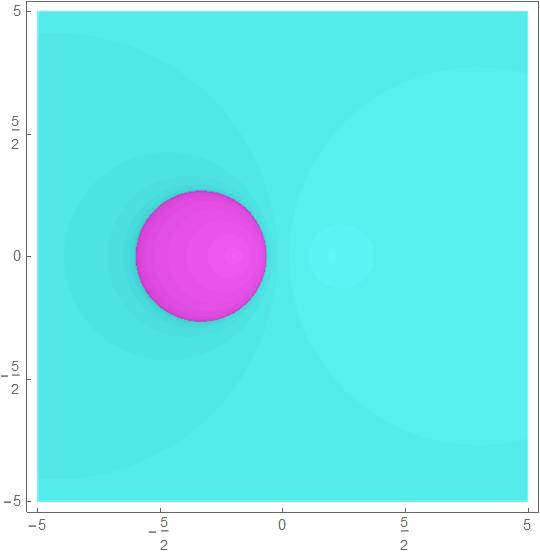
\includegraphics[width=0.98\textwidth]{fuentes/articulo-cuadraticos/imagenes/sch_m_2n_1.jpg}
\small Schröder: $m=2, \, n=1.$
\end{minipage}\hfill
\begin{minipage}[t]{0.45\textwidth}
\centering
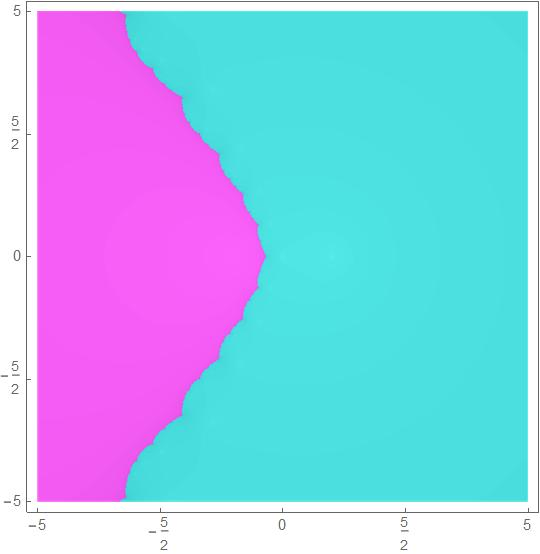
\includegraphics[width=0.98\textwidth]{fuentes/articulo-cuadraticos/imagenes/newton_m_2n_1.jpg}
\small Newton: $m=2, \, n=1.$
\end{minipage}

\vspace{0.5cm}

\begin{minipage}[t]{0.45\textwidth}
\centering
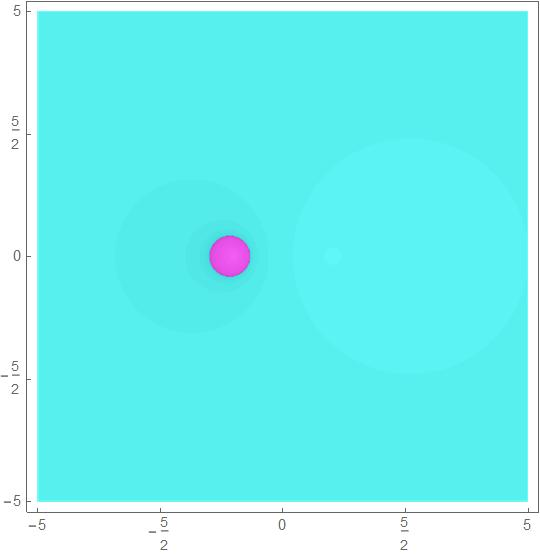
\includegraphics[width=0.98\textwidth]{fuentes/articulo-cuadraticos/imagenes/sch_m_5n_1.jpg}
\small Schröder: $m=5, \, n=1.$
\end{minipage}\hfill
\begin{minipage}[t]{0.45\textwidth}
\centering
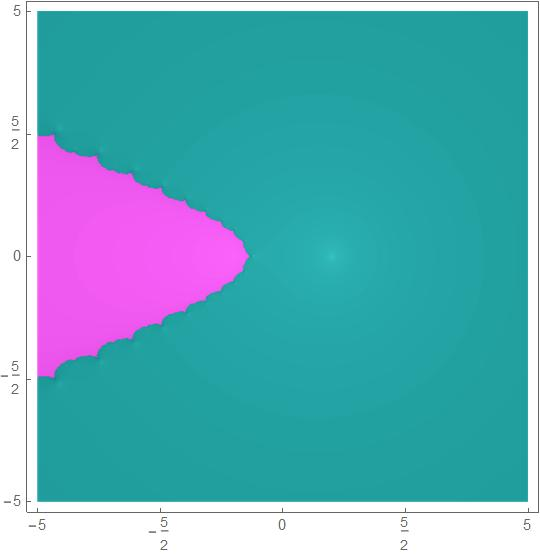
\includegraphics[width=0.98\textwidth]{fuentes/articulo-cuadraticos/imagenes/newton_m_5n_1.jpg}
\small Newton: $m=5, \, n=1.$
\end{minipage}

\vspace{0.5cm}

\begin{minipage}[t]{0.45\textwidth}
\centering
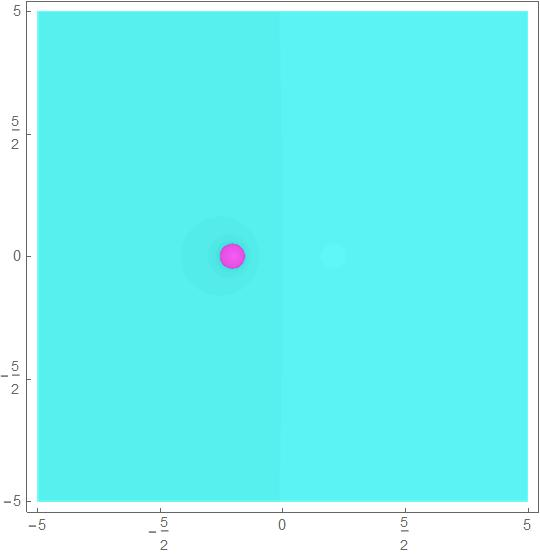
\includegraphics[width=0.98\textwidth]{fuentes/articulo-cuadraticos/imagenes/sch_m_8n_1.jpg}
\small Schröder: $m=8, \, n=1.$
\end{minipage}\hfill
\begin{minipage}[t]{0.45\textwidth}
\centering
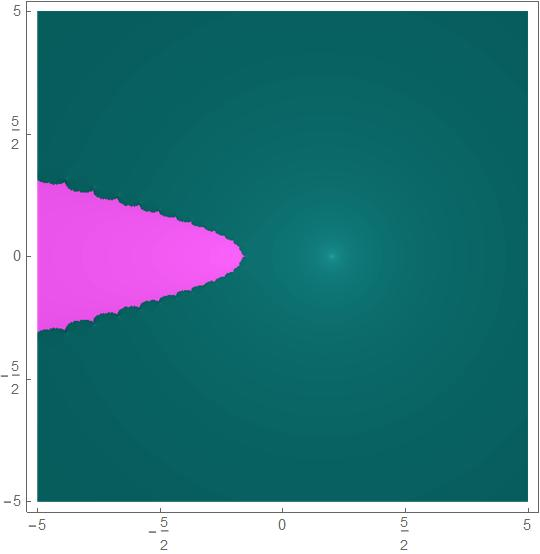
\includegraphics[width=0.98\textwidth]{fuentes/articulo-cuadraticos/imagenes/newton_m_8n_1.jpg}
\small Newton: $m=8, \, n=1.$
\end{minipage}

\caption{Cuencas de atracción de los métodos de Schröder y Newton aplicados a polinomios $(z-1)^m(z+1)^n$ para $n=1$ y $m=2, 5, 8$. Se aprecia cómo el conjunto de Julia del método de Schröder (un círculo) tiende a colapsar en la raíz $z=-1$ de menor multiplicidad. En el caso de Newton, el Julia es una ``parábola deformada'' cuyo vértice se aproxima también a $z=-1$ y cuyo ``ancho'' tiende a cero. La cuenca de la raíz múltiple $z=1$ invade progresivamente el plano.}
\label{fig:p_creciente}
\end{figure}

\subsubsection{Caso: $p=m/n$ próximo a 1}

En la Figura~\ref{fig:p_proximo1} se muestra qué ocurre cuando $p=m/n\approx 1$, es decir, cuando las multiplicidades son similares. Se consideran polinomios $(z-1)^m(z+1)^n$ con $n=6$ y $m=6, 7, 8$.

\begin{figure}[H]
\centering 
\begin{minipage}[t]{0.45\textwidth}
\centering
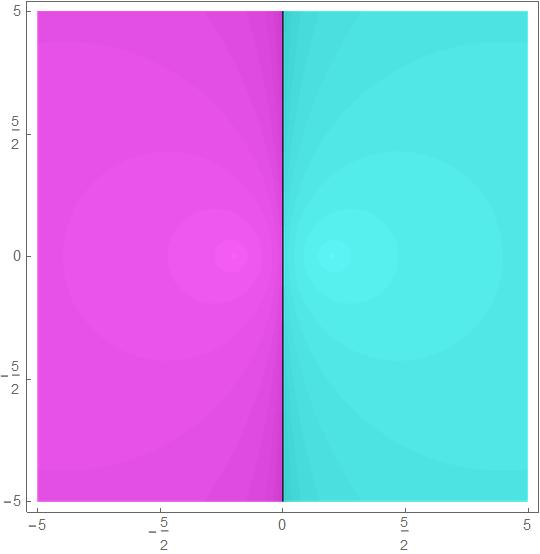
\includegraphics[width=0.98\textwidth]{fuentes/articulo-cuadraticos/imagenes/sch_n_6_m_6.jpg}
\small Schröder: $m=6, \, n=6.$
\end{minipage}\hfill
\begin{minipage}[t]{0.45\textwidth}
\centering
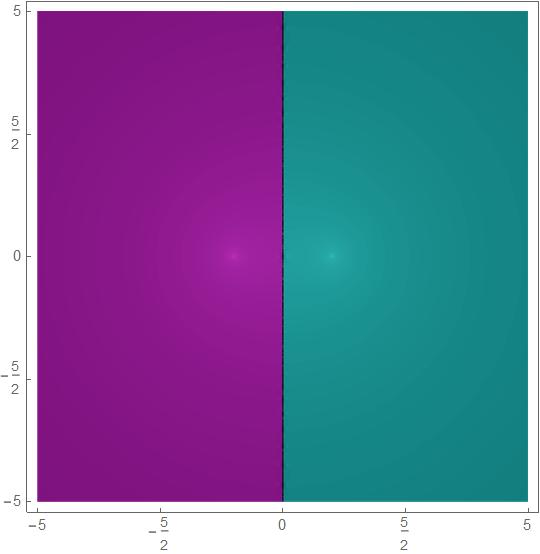
\includegraphics[width=0.98\textwidth]{fuentes/articulo-cuadraticos/imagenes/newton_n_6_m_6.jpg}
\small Newton: $m=6, \, n=6.$
\end{minipage}

\vspace{0.5cm}

\begin{minipage}[t]{0.45\textwidth}
\centering
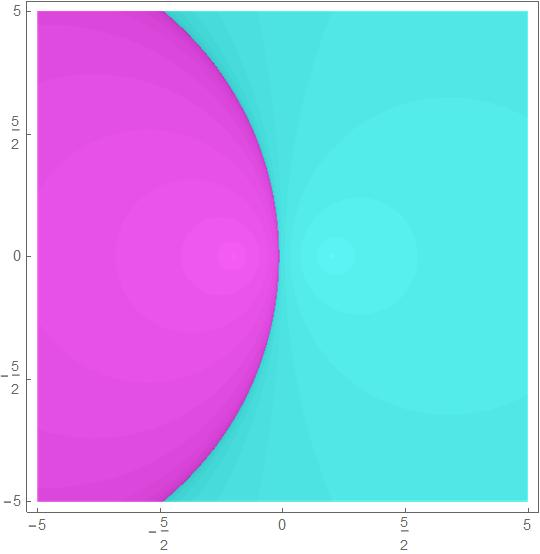
\includegraphics[width=0.98\textwidth]{fuentes/articulo-cuadraticos/imagenes/sch_m_7n_6.jpg}
\small Schröder: $m=7, \, n=6.$
\end{minipage}\hfill
\begin{minipage}[t]{0.45\textwidth}
\centering
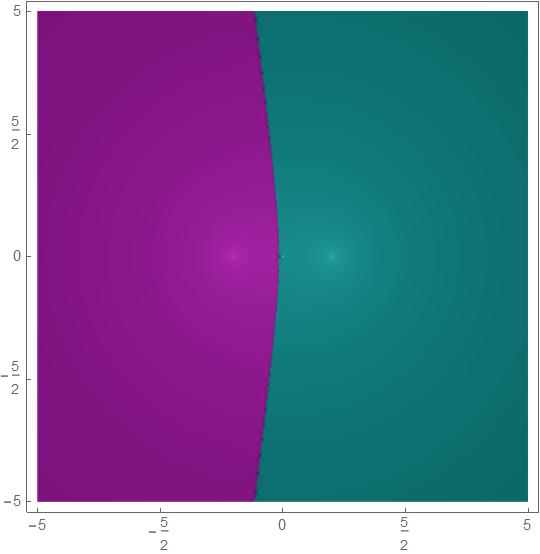
\includegraphics[width=0.98\textwidth]{fuentes/articulo-cuadraticos/imagenes/newton_m_7n_6.jpg}
\small Newton: $m=7, \, n=6.$
\end{minipage}

\vspace{0.5cm}

\begin{minipage}[t]{0.45\textwidth}
\centering
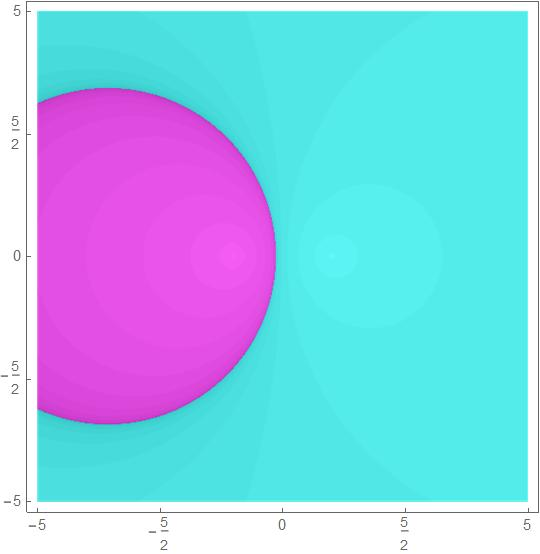
\includegraphics[width=0.98\textwidth]{fuentes/articulo-cuadraticos/imagenes/sch_m_8n_6.jpg}
\small Schröder: $m=8, \, n=6.$
\end{minipage}\hfill
\begin{minipage}[t]{0.45\textwidth}
\centering
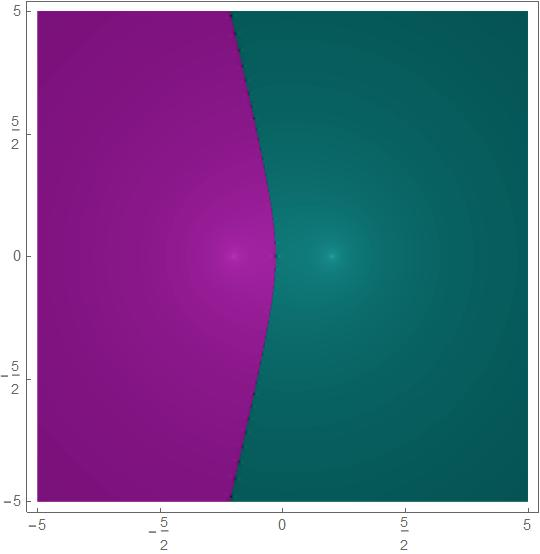
\includegraphics[width=0.98\textwidth]{fuentes/articulo-cuadraticos/imagenes/newton_m_8n_6.jpg}
\small Newton: $m=8, \, n=6.$
\end{minipage}

\caption{Cuencas de atracción de los métodos de Schröder y Newton aplicados a polinomios $(z-1)^m(z+1)^n$ para $n=6$ y $m=6, 7, 8$. El conjunto de Julia del método de Schröder son círculos que crecen a medida que $p$ se aproxima a 1, tendiendo a ``explotar'' en el eje imaginario cuando $p=1$ (caso $m=n=6$). Para Newton, la ``parábola deformada'' tiene su vértice cerca de $z=0$ y su ``ancho'' crece, tendiendo al eje imaginario cuando $p=1$.}
\label{fig:p_proximo1}
\end{figure}

\subsubsection{Caso: razón constante $p=2$}

La Figura~\ref{fig:p_constante} muestra el círculo correspondiente al conjunto de Julia del método de Schröder para polinomios con $p=m/n=2$, independientemente de los valores específicos de $m$ y $n$. También se aprecia que para Newton, aunque los valores absolutos de $m$ y $n$ influyen en la suavidad del Julia, la estructura general permanece similar para la misma razón $p$.

\begin{figure}[H]
\centering 
\begin{minipage}[t]{0.4\textwidth}
\centering
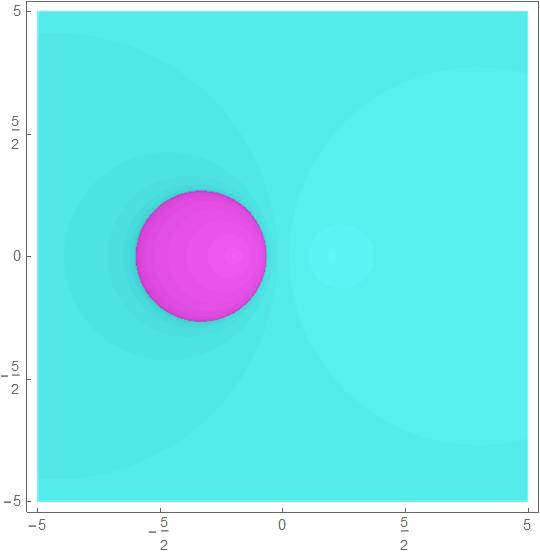
\includegraphics[width=0.88\textwidth]{fuentes/articulo-cuadraticos/imagenes/sch_m_4n_2.jpg}
\small Schröder: $p=m/n=2.$
\end{minipage}\hfill
\begin{minipage}[t]{0.4\textwidth}
\centering
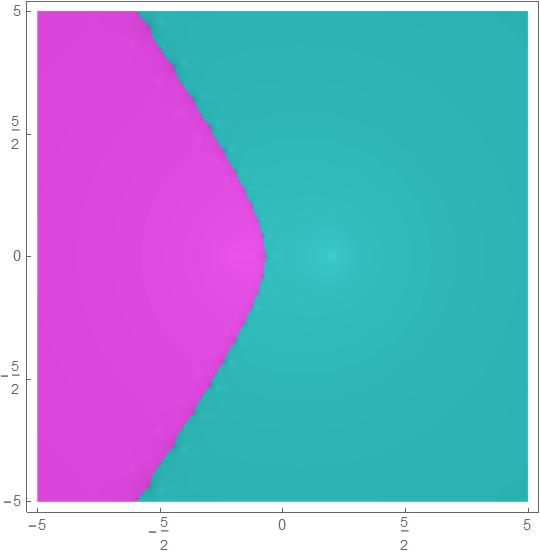
\includegraphics[width=0.88\textwidth]{fuentes/articulo-cuadraticos/imagenes/newton_m_4n_2.jpg}
\small Newton: $m=4, \, n=2.$
\end{minipage}

\vspace{0.5cm}

\begin{minipage}[t]{0.4\textwidth}
\centering
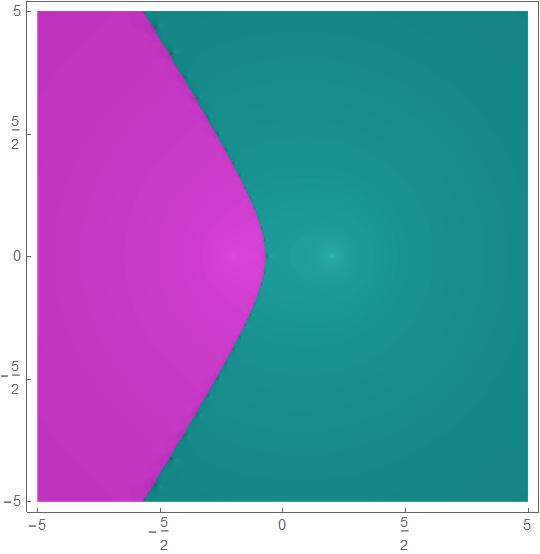
\includegraphics[width=0.88\textwidth]{fuentes/articulo-cuadraticos/imagenes/newton_m_6n_3.jpg}
\small Newton: $m=6, \, n=3.$
\end{minipage}\hfill
\begin{minipage}[t]{0.4\textwidth}
\centering
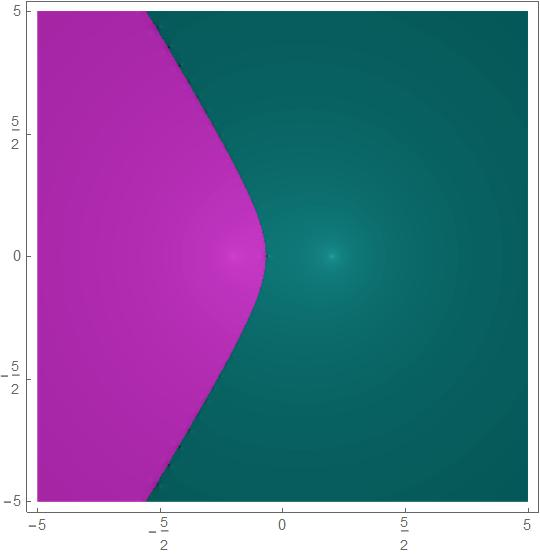
\includegraphics[width=0.88\textwidth]{fuentes/articulo-cuadraticos/imagenes/newton_m_8n_4.jpg}
\small Newton: $m=8, \, n=4.$
\end{minipage}

\caption{La primera imagen muestra la cuenca de atracción del método de Schröder aplicado a polinomios $(z-1)^m(z+1)^n$ con $p=m/n=2$. El conjunto de Julia es el mismo círculo para todos los pares $(m,n)$ con esta razón. Las otras imágenes muestran las cuencas del método de Newton para distintos valores de $m$ y $n$ con $p=m/n=2$. Se observa que la ``parábola deformada'' tiende a ser más suave conforme aumentan $m$ y $n$.}
\label{fig:p_constante}
\end{figure}

\subsubsection{Caso: raíces no reales}

Finalmente, en la Figura~\ref{fig:raices_complejas} se muestra un ejemplo con raíces no reales: $(z-1)^2(z-i)$. Se aprecia la pérdida de simetría respecto al eje imaginario, siendo ahora la recta equidistante entre las raíces la que juega el papel de eje de referencia.

\begin{figure}[H]
\centering 
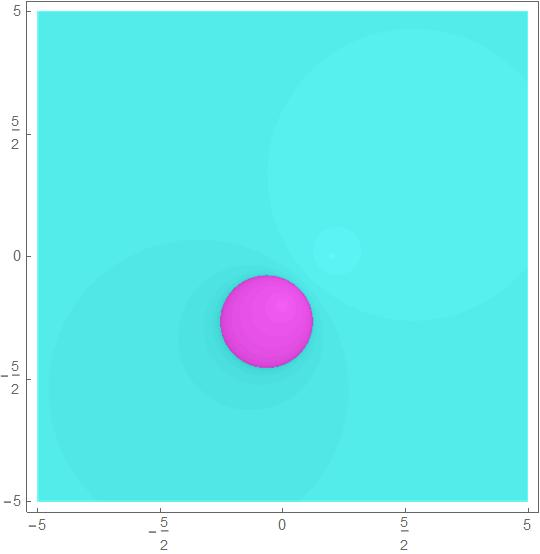
\includegraphics[width=0.4\textwidth]{fuentes/articulo-cuadraticos/imagenes/sch-i_m2_n1.jpg}\quad 
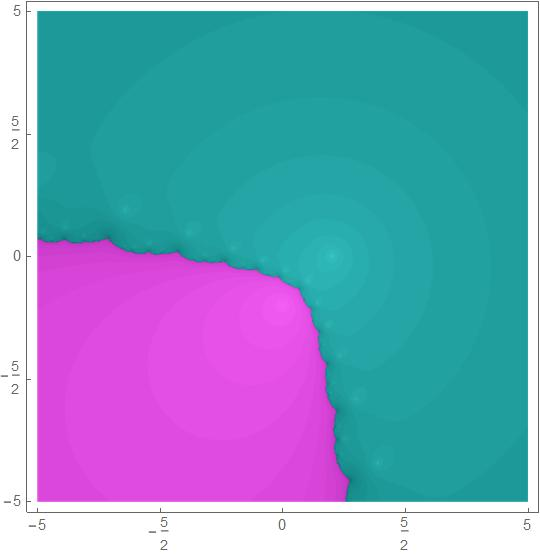
\includegraphics[width=0.4\textwidth]{fuentes/articulo-cuadraticos/imagenes/newton1-i_m2_n1.jpg}
\caption{Cuencas de atracción de los métodos de Schröder (izquierda) y Newton (derecha) aplicados al polinomio $(z-1)^2(z-i)$. El conjunto de Julia del método de Schröder sigue siendo un círculo dado por el Teorema~\ref{teo:julia_general}, pero ahora desplazado y sin la simetría respecto al eje imaginario. La frontera es ahora la perpendicular a la recta que une las raíces $z=1$ y $z=i$.}
\label{fig:raices_complejas}
\end{figure}

\subsection{Comparación con el método de Newton}

El análisis anterior permite establecer una comparación sistemática entre los métodos de Schröder y Newton para polinomios con dos raíces de multiplicidades arbitrarias.

\subsubsection{Naturaleza del conjunto de Julia}

\begin{itemize}
\item \textbf{Schröder:} El conjunto de Julia es siempre un círculo (o una recta en el caso límite $m=n$), cuya posición y radio están dados explícitamente por el Teorema~\ref{teo:julia_general}. Esta geometría simple facilita el análisis teórico y la predicción del comportamiento.

\item \textbf{Newton:} El conjunto de Julia tiene forma de ``parábola deformada'' cuya caracterización exacta es más compleja. Su forma depende no solo de la razón $p=m/n$ sino también de los valores absolutos de $m$ y $n$.
\end{itemize}

\subsubsection{Distribución de las cuencas de atracción}

\begin{itemize}
\item \textbf{Caso $m=n$:} Ambos métodos tienen el mismo conjunto de Julia (la bisectriz entre las raíces) y las mismas cuencas de atracción (los dos semiplanos correspondientes).

\item \textbf{Caso $m>n$:} 
\begin{itemize}
\item Para Schröder, la cuenca de la raíz de menor multiplicidad está completamente contenida en un disco, rodeada por la cuenca de la raíz de mayor multiplicidad.
\item Para Newton, la cuenca de la raíz de menor multiplicidad tiene una estructura más compleja en forma de franja acotada por la ``parábola deformada'', pero que se extiende hasta el infinito en ciertas direcciones.
\end{itemize}
\end{itemize}

\subsubsection{Coste computacional y orden de convergencia}

\begin{itemize}
\item \textbf{Newton:} Orden de convergencia 2 para raíces simples, lineal para raíces múltiples. Coste: 1 evaluación de $f$ y 1 de $f'$ por iteración.

\item \textbf{Schröder:} Orden de convergencia 2 incluso para raíces múltiples (ventaja importante). Coste: 1 evaluación de $f$, 1 de $f'$ y 1 de $f''$ por iteración (coste similar a métodos de orden 3 de la familia Chebyshev-Halley).
\end{itemize}

El método de Schröder resulta especialmente ventajoso cuando se sabe de antemano que existen raíces múltiples, ya que mantiene convergencia cuadrática sin necesidad de conocer la multiplicidad.

\section{Polinomios cúbicos: estudio del plano de parámetros}

Extendemos ahora el estudio a polinomios cúbicos con tres raíces distintas. Este caso presenta una complejidad considerablemente mayor y revela fenómenos dinámicos inesperados que no aparecen en el caso de dos raíces.

\subsection{Polinomios cúbicos con tres raíces simples}

Consideramos ahora polinomios de la forma
\begin{equation}
p(z)=(z-a)(z-b)(z-c), \quad a,b,c\in\C, \quad a\ne b\ne c.
\label{eq:poly_cubico}
\end{equation}

A diferencia del caso de dos raíces, donde las cuencas de atracción estaban delimitadas por círculos y rectas, en el caso cúbico aparecen estructuras fractales y regiones de no convergencia. En la Figura~\ref{fig:cuenca_cubica_1} se muestran las cuencas de atracción del polinomio $(z^2-1)(z-3-i)$.

\begin{figure}[H]
\centering 
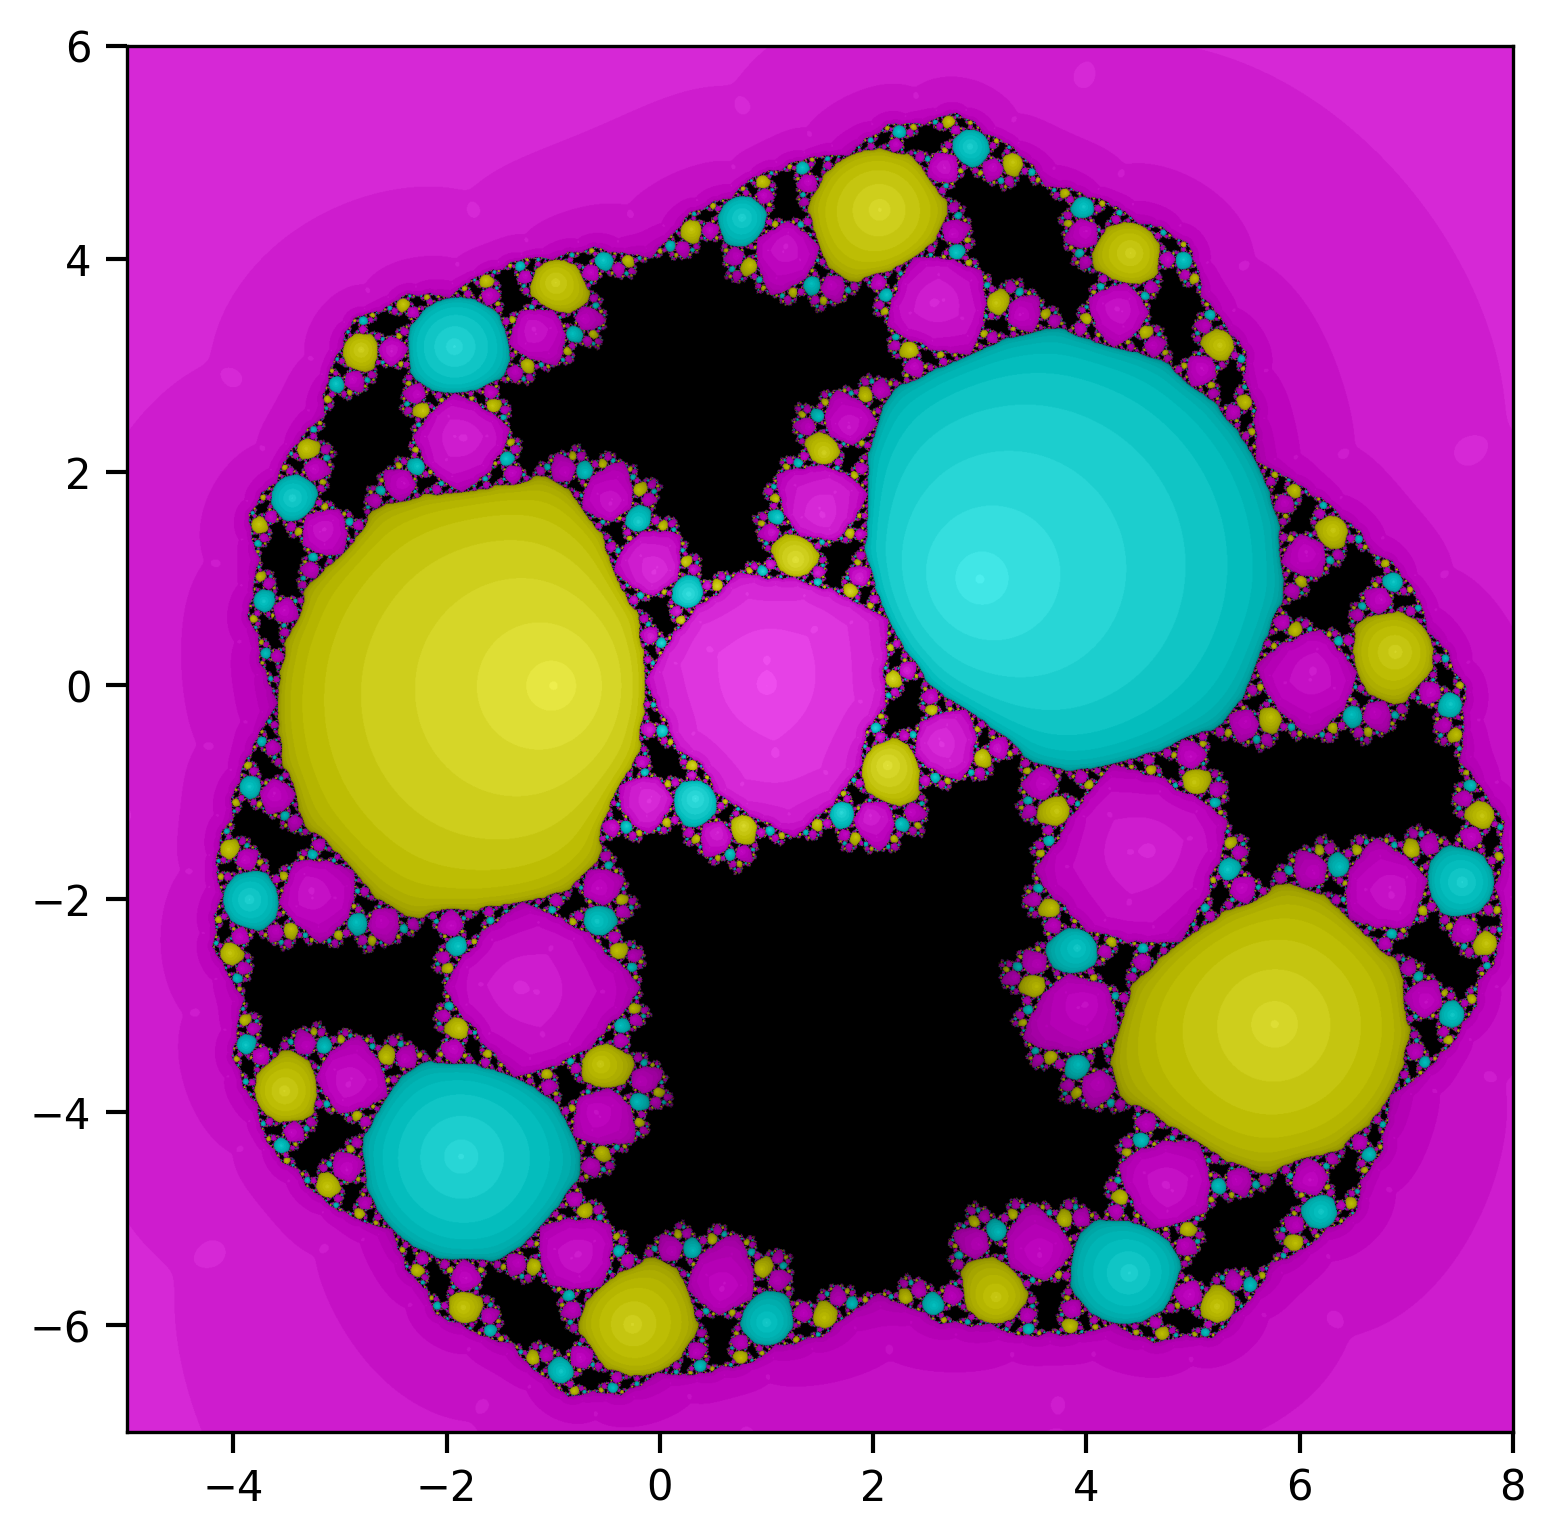
\includegraphics[width=0.6\textwidth]{img/sch_3+i.png}
\caption{Cuencas de atracción del método de Schröder aplicado a $p(z)=(z^2-1)(z-3-i)$. En cyan la cuenca de atracción de $z=1$, en magenta la de $z=-1$ y en amarillo la de $z=3+i$. Las zonas blancas representan puntos que no convergen a ninguna raíz tras un número determinado de iteraciones.}
\label{fig:cuenca_cubica_1}
\end{figure}

Observamos dos fenómenos importantes:
\begin{enumerate}
\item Existen regiones extensas (en blanco) donde el método no converge a ninguna raíz.
\item La cuenca de atracción de la raíz $z=1$ (en cyan) domina ampliamente el plano, un comportamiento distinto al del método de Newton donde todas las cuencas se extienden hasta el infinito.
\end{enumerate}

\subsection{Puntos críticos y el teorema de Fatou-Julia}

Para entender el comportamiento observado, es fundamental analizar los puntos críticos de la función de iteración.

Un punto $\zeta\in\C$ se dice \textbf{punto crítico} de una función racional $R$ si la inyectividad de $R$ falla en un entorno de $\zeta$. Equivalentemente, $\zeta$ es punto crítico si $R'(\zeta)=0$ o si $R$ no está definida en $\zeta$.

\begin{teorema}[Teorema de Fatou-Julia]
\label{teo:fatou_julia}
Todo ciclo atractor de una función racional atrae al menos un punto crítico de ésta.
\end{teorema}

Este resultado es clave: las zonas blancas en la Figura~\ref{fig:cuenca_cubica_1} indican la presencia de ciclos atractores que no son las raíces del polinomio. Estos ciclos atraen alguno de los puntos críticos libres (aquellos que no son raíces).

\subsection{Reducción a una familia uniparamétrica}

Similar al análisis del caso cuadrático, podemos simplificar el estudio mediante una transformación afín.

\begin{teorema}
Sea $p(z)=(z-a)(z-b)(z-c)$ un polinomio cúbico con raíces distintas. Existe una transformación afín $A(z)=\alpha z+\beta$ tal que el polinomio transformado tiene la forma $q(z)=(z^2-1)(z-\lambda)$ con $\lambda\in\C$. Además, la función de iteración $S_p$ es conjugada a $S_q$ mediante $A$:
$$
A\circ S_q\circ A^{-1}=S_p.
$$
\end{teorema}

Los parámetros de la transformación están dados por:
$$
\alpha=\frac{a-b}{2}, \quad \beta=\frac{a+b}{2}, \quad \lambda=\frac{2c-a-b}{a-b}.
$$

Este resultado reduce el estudio dinámico de todos los polinomios cúbicos con tres raíces distintas al estudio de la familia uniparamétrica
$$
P_\lambda=\{(z^2-1)(z-\lambda), \quad \lambda\in\C\}.
$$

\subsection{Análisis de puntos críticos}

La función de iteración de Schröder para $p_\lambda(z)=(z^2-1)(z-\lambda)$ es:
$$
S_{p_\lambda}(z)=\frac{4\lambda^2 z+\lambda(z^4-10z^2+1)+4z^3}{2\lambda^2(z^2+1)-4\lambda(z^3+z)+3z^4+1}.
$$

Su derivada es:
$$
S'_{p_\lambda}(z)=-\frac{4(z^2-1)(z-\lambda)(-2\lambda^3-2\lambda+\lambda^2 z^3+3z^3-12\lambda z^2+9\lambda^2 z+3z)}{(2\lambda^2+3z^4-4\lambda z^3+2\lambda^2 z^2-4\lambda z+1)^2}.
$$

Las raíces $-1$, $1$ y $\lambda$ son puntos críticos que convergen a sí mismas. Los puntos críticos \emph{libres} son las raíces del numerador:
$$
-2\lambda^3-2\lambda+\lambda^2 z^3+3z^3-12\lambda z^2+9\lambda^2 z+3z=0.
$$

Esta ecuación cúbica en $z$ tiene tres soluciones $\zeta_1(\lambda)$, $\zeta_2(\lambda)$ y $\zeta_3(\lambda)$ (expresiones complejas que se pueden calcular explícitamente mediante las fórmulas de Cardano).

\subsection{El plano de parámetros}

Para cada valor de $\lambda\in\C$, estudiamos el comportamiento de las órbitas de los tres puntos críticos libres. Coloreamos el plano complejo (plano de parámetros) según el destino de cada punto crítico:
\begin{itemize}
\item \textbf{Cyan}: el punto crítico converge a la raíz $z=1$.
\item \textbf{Magenta}: el punto crítico converge a la raíz $z=-1$.
\item \textbf{Amarillo}: el punto crítico converge a la raíz $z=\lambda$.
\item \textbf{Negro}: el punto crítico no converge a ninguna raíz (indica ciclo atractor extraño).
\end{itemize}

En las Figuras~\ref{fig:plano_param_1}, \ref{fig:plano_param_2} y~\ref{fig:plano_param_3} se muestran los planos de parámetros para cada uno de los tres puntos críticos libres.

\begin{figure}[H]
\centering 
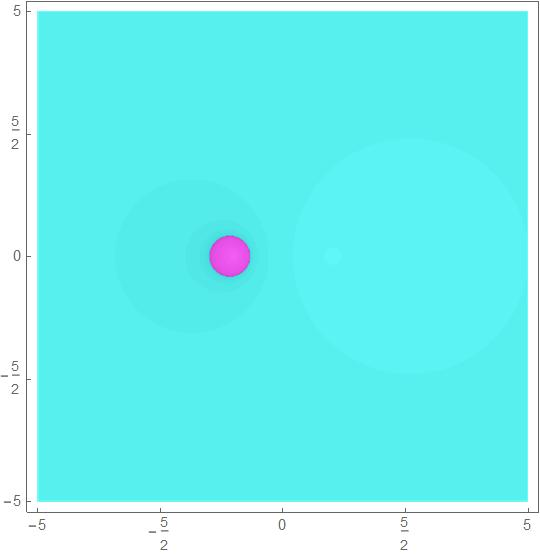
\includegraphics[width=0.55\textwidth]{fuentes/articulo-cuadraticos/imagenes/sch_m_5n_1.jpg}
\caption{Plano de parámetros para el punto crítico libre $\zeta_1(\lambda)$. En cyan los valores de $\lambda$ para los que $\zeta_1$ converge a $1$, en magenta a $-1$, en amarillo a $\lambda$, y en negro cuando no converge a ninguna raíz.}
\label{fig:plano_param_1}
\end{figure}

\begin{figure}[H]
\centering 
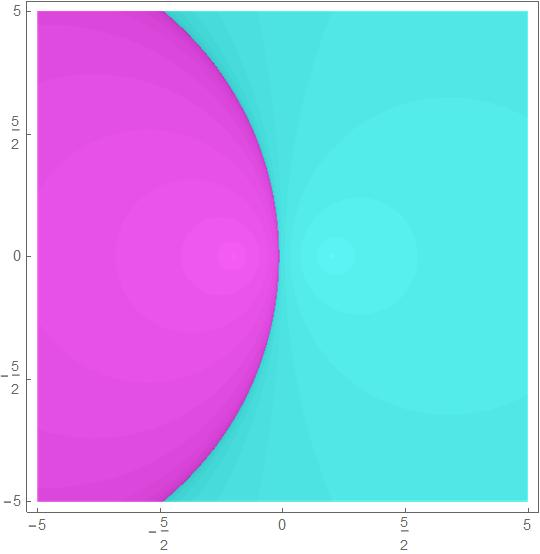
\includegraphics[width=0.55\textwidth]{fuentes/articulo-cuadraticos/imagenes/sch_m_7n_6.jpg}
\caption{Plano de parámetros para el punto crítico libre $\zeta_2(\lambda)$.}
\label{fig:plano_param_2}
\end{figure}

\begin{figure}[H]
\centering 
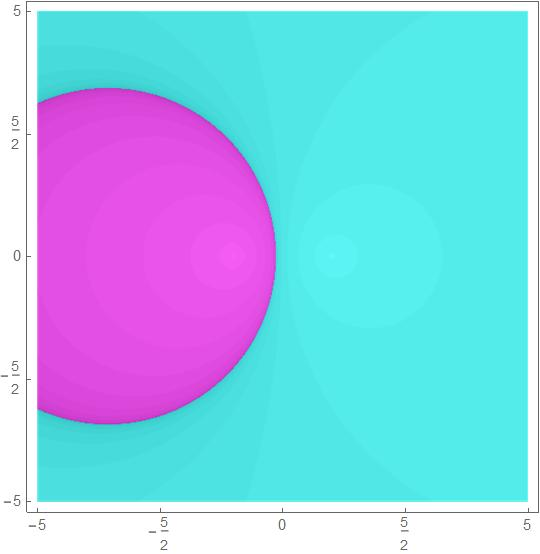
\includegraphics[width=0.55\textwidth]{fuentes/articulo-cuadraticos/imagenes/sch_m_8n_6.jpg}
\caption{Plano de parámetros para el punto crítico libre $\zeta_3(\lambda)$.}
\label{fig:plano_param_3}
\end{figure}

Las zonas negras en estas figuras corresponden a valores de $\lambda$ para los cuales existe al menos un ciclo atractor que no es una raíz. Estos son precisamente los polinomios para los que el método de Schröder presenta zonas de no convergencia en sus cuencas de atracción.

\subsection{Comparación con el método de Newton}

El método de Newton aplicado al mismo polinomio $p_\lambda(z)=(z^2-1)(z-\lambda)$ tiene función de iteración:
$$
N_{p_\lambda}(z)=\frac{-\lambda+2z^3-\lambda z^2}{3z^2-2\lambda z-1}.
$$

Su derivada es:
$$
N'_{p_\lambda}(z)=\frac{2(z^2-1)(z-\lambda)(3z-\lambda)}{(3z^2-2\lambda z-1)^2}.
$$

El método de Newton tiene un único punto crítico libre: $\zeta=\lambda/3$. Su plano de parámetros se muestra en la Figura~\ref{fig:plano_param_newton}.

\begin{figure}[H]
\centering 
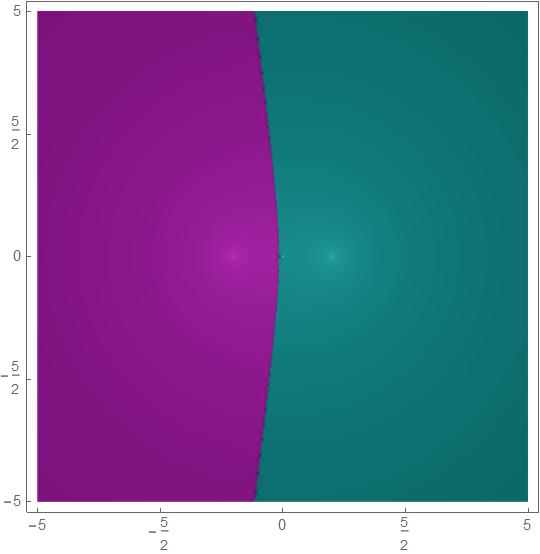
\includegraphics[width=0.6\textwidth]{fuentes/articulo-cuadraticos/imagenes/newton_m_7n_6.jpg}
\caption{Plano de parámetros del método de Newton para $p_\lambda(z)=(z^2-1)(z-\lambda)$. El método de Newton tiene un único punto crítico libre, lo que simplifica considerablemente el análisis.}
\label{fig:plano_param_newton}
\end{figure}

Comparando con las Figuras~\ref{fig:plano_param_1}--\ref{fig:plano_param_3}, observamos que:
\begin{itemize}
\item Newton tiene un solo punto crítico libre, Schröder tiene tres.
\item Las zonas negras (no convergencia) son mucho más extensas en Schröder que en Newton.
\item La estructura del plano de parámetros es más simple para Newton.
\end{itemize}

\subsection{Caso especial: raíces formando un triángulo equilátero}

Un caso particularmente interesante ocurre cuando $\lambda=\sqrt{3}i$, pues las tres raíces $1$, $-1$ y $\sqrt{3}i$ forman un triángulo equilátero en el plano complejo.

Para este valor, la derivada de la función de iteración se simplifica a:
$$
S'_{p_{\sqrt{3}i}}(z)=-\frac{16(z-1)(z+1)(z-\sqrt{3}i)}{(3iz^3+3\sqrt{3}z^2-3iz+5\sqrt{3})^2}.
$$

En este caso, los únicos puntos críticos son las propias raíces. Por el Teorema~\ref{teo:fatou_julia}, no pueden existir ciclos atractores extraños, y por tanto todas las órbitas convergen a alguna de las tres raíces. Las cuencas de atracción para este caso se muestran en las Figuras~\ref{fig:cuenca_triangulo_1} y~\ref{fig:cuenca_triangulo_2}.

\begin{figure}[H]
\centering 
\begin{minipage}[b]{0.48\textwidth}
\centering
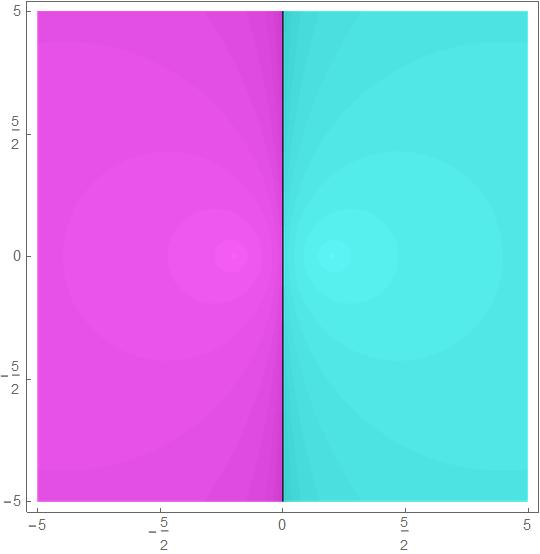
\includegraphics[width=\textwidth]{fuentes/articulo-cuadraticos/imagenes/sch_n_6_m_6.jpg}
\caption{Cuencas de atracción para $\lambda=\sqrt{3}i$ en la región $[-5,5]\times[-5i,5i]$.}
\label{fig:cuenca_triangulo_1}
\end{minipage}
\hfill
\begin{minipage}[b]{0.48\textwidth}
\centering
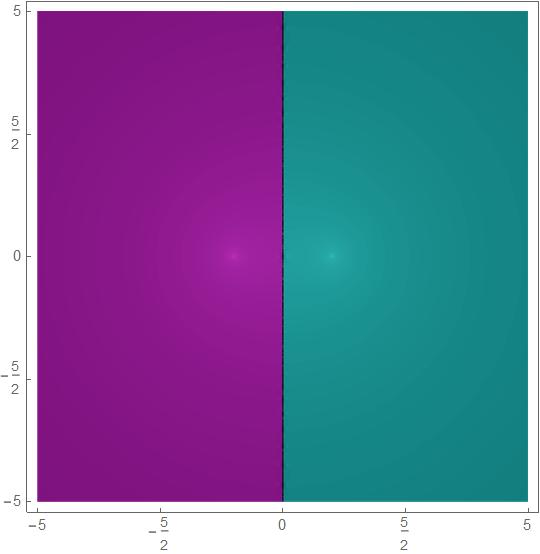
\includegraphics[width=\textwidth]{fuentes/articulo-cuadraticos/imagenes/newton_n_6_m_6.jpg}
\caption{Mismo caso en la región $[-100,100]\times[-100i,100i]$.}
\label{fig:cuenca_triangulo_2}
\end{minipage}
\end{figure}

\subsection{Observaciones dinámicas adicionales}

Los casos especiales analizados ($\lambda=\sqrt{3}i$ y $\lambda=0$) revelan la riqueza del espacio de parámetros. Mientras que para algunos valores de $\lambda$ todas las órbitas convergen a raíces (caso $\lambda=\sqrt{3}i$), para otros valores aparecen ciclos atractores que no son raíces (caso $\lambda=0$ con el 2-ciclo $\{i,-i\}$).

Este comportamiento contrasta notablemente con el caso de dos raíces, donde todos los puntos del plano complejo (excepto el conjunto de Julia) convergen necesariamente a una de las raíces. La presencia de tres puntos críticos libres en el caso cúbico, frente a ninguno en el caso de dos raíces, explica esta mayor complejidad dinámica.

\section{Conclusiones}

El estudio dinámico del método de Schröder en el plano complejo revela comportamientos cualitativamente distintos según el número de raíces del polinomio.

\subsection{Síntesis de resultados para dos raíces}

Para polinomios con dos raíces de multiplicidades arbitrarias:

\begin{enumerate}
\item El conjunto de Julia es siempre un círculo (o una recta cuando las multiplicidades son iguales), cuya ecuación explícita está dada por los Teoremas~\ref{teo:julia_canonico} y~\ref{teo:julia_general}.

\item La razón $p=m/n$ entre multiplicidades es el parámetro fundamental que determina la geometría del Julia.

\item Existe un comportamiento límite bien definido: colapso en la raíz simple cuando $p\to\infty$, y explosión en la bisectriz cuando $p\to 1^+$.

\item La comparación con Newton muestra que Schröder tiene conjuntos de Julia más simples geométricamente (círculos vs. parábolas deformadas).

\item El método de Schröder mantiene convergencia cuadrática para raíces múltiples, ventaja importante frente a Newton.
\end{enumerate}

\subsection{Síntesis de resultados para polinomios cúbicos}

Para polinomios cúbicos con tres raíces simples:

\begin{enumerate}
\item La presencia de tres puntos críticos libres (frente a ninguno en el caso de dos raíces) introduce complejidad dinámica fundamental.

\item Aparecen regiones extensas de no convergencia, correspondientes a ciclos atractores que no son raíces.

\item El plano de parámetros revela una estructura compleja: para ciertos valores de $\lambda$ existen ciclos atractores extraños, mientras que para otros todas las órbitas convergen a raíces.

\item El caso $\lambda=\sqrt{3}i$ (triángulo equilátero) es excepcional: no tiene puntos críticos libres y todas las órbitas convergen a alguna raíz.

\item El caso $\lambda=0$ exhibe un 2-ciclo superatractor en $\{i,-i\}$, ilustrando claramente la existencia de atractores no triviales.

\item El método de Newton, con un solo punto crítico libre, presenta un plano de parámetros más simple y menos zonas de no convergencia.
\end{enumerate}

\subsection{Implicaciones prácticas}

Estos resultados tienen importantes implicaciones para el uso del método de Schröder:

\begin{itemize}
\item \textbf{Para polinomios con dos raíces:} El método es altamente predecible. La geometría circular del Julia facilita la selección de condiciones iniciales apropiadas. Es particularmente ventajoso en presencia de multiplicidades.

\item \textbf{Para polinomios cúbicos:} La posible existencia de ciclos atractores extraños requiere precaución. El método puede no converger a ninguna raíz incluso con condiciones iniciales aparentemente razonables. Es recomendable implementar criterios de detección de no convergencia.

\item \textbf{Comparación con Newton:} Mientras que Schröder supera a Newton en presencia de raíces múltiples, para polinomios con múltiples raíces simples, Newton puede ser más robusto debido a su menor número de puntos críticos libres.
\end{itemize}

\section{El punto del infinito en el método de Schröder}

Una característica distintiva del método de Schröder, que lo diferencia de otros métodos iterativos como Newton, Halley o Chebyshev, es el comportamiento del punto del infinito. Mientras que en estos últimos métodos el infinito es un punto fijo repulsor, en el método de Schröder el infinito no es punto fijo, lo que introduce fenómenos dinámicos únicos que merecen un análisis detallado.

\subsection{Grado del método de Schröder}

En el estudio del comportamiento dinámico de métodos iterativos para resolver ecuaciones polinómicas, uno de los primeros pasos consiste en determinar el grado de la aplicación racional asociada. Si bien es relativamente sencillo establecer cotas superiores para este grado, el cálculo del valor exacto requiere la introducción del concepto de \emph{punto crítico especial}, tal como fue empleado por Nayak y Pal en su análisis de la aplicación racional asociada al método de Chebyshev.

\begin{dfn}[Punto crítico especial]
Dado un polinomio complejo $p(z)$, un punto crítico $c\in\mathbb{C}$ se denomina especial si $p(c)\ne 0$ pero $p''(c) = 0$.
\end{dfn}

Para mayor comodidad, escribimos la aplicación de iteración del método de Schröder de la forma equivalente
\begin{equation}
S_p(z)=z -\frac{p(z)p'(z)}{p'(z)^2- p(z)p''(z)}.
\label{eq:sch_alt_form}
\end{equation}

\begin{teorema}\label{teo:grado_schroder}
Sea $S_p(z)$ la aplicación de iteración del método de Schröder para resolver ecuaciones polinómicas, escrita como en \eqref{eq:sch_alt_form}. Entonces el grado de la aplicación racional $S_{p}(z)$ es
$$\deg(S_{p}(z)) =2r+s-C-2,$$
donde
\begin{itemize}
\item $r$ es el número de raíces distintas de $p(z)$.
\item $s$ es el número de puntos críticos especiales de $p(z)$.
\item $C=c_1+\cdots+c_k$ es la suma de multiplicidades de todos los puntos críticos especiales.
\end{itemize}
\end{teorema}

\begin{proof}
Comenzamos observando que $\deg(\text{Num}(S_p(z)))\le \deg(\text{Den}(S_p(z)))\le 2d-2$. En efecto, para un polinomio mónico general de la forma $p(z)=z^d +a_{d-1} z^{d-1} + \cdots$ es fácil demostrar, tras algunas manipulaciones algebraicas, que
$$ \text{Num}(S_p(z))=zp'(z)^2-zp(z)p''(z)-p(z)p'(z)=-a_{d-1}z^{2d-2}+P_{2d-3}(z), $$
$$ \text{Den}(S_p(z))=p'(z)^2-p(z)p''(z)=-dz^{2d-2}+Q_{2d-3}(z),$$
donde $P_{2d-3}(z)$ y $Q_{2d-3}(z)$ son polinomios de grado $2d-3$.

Consecuentemente, $\deg(S_p(z))\le 2d-2$. Además, $\deg(S_p(z))< 2d-2$ si $\text{Num}(S_p(z))$ y $\text{Den}(S_p(z))$ tienen raíces comunes. Para calcular el grado exacto de $S_p(z)$, debemos analizar $\deg(\text{Den}(S_p(z)))$.

La demostración se basa en las siguientes factorizaciones de los polinomios $p(z)$, $p'(z)$ y $p''(z)$:
\[
p(z)=\prod_{i=1}^m(z-\alpha_i)\prod_{j=1}^n(z-\beta_j)^{b_j},\quad b_j\ge 2,
\]
con $\deg(p)=m+B$, $B=\sum_{j=1}^n b_j.$ Teniendo en cuenta que una raíz de $p(z)$ con multiplicidad $k\ge 1$ es raíz de $p'(z)$ con multiplicidad $k-1$ (y un criterio similar para $p''(z)$), tenemos
$$p'(z)=g(z)\prod_{j=1}^n(z-\beta_j)^{b_j-1},$$
$$p''(z)=h(z)\prod_{j=1}^n(z-\beta_j)^{b_j-2},$$
donde $g(z)$ y $h(z)$ son polinomios que satisfacen $g(\alpha_i)\ne 0$, $i=1,\dots, m$, $g(\beta_j)\ne0$ y $h(\beta_j)\ne 0$ para $j=1,\dots, n$.

Además, $\deg(g)=\deg(p')-B+n=m+n-1$ y el coeficiente líder de $g(z)$ es $d$; $\deg(h)=\deg(p'')-B+2n=m+2n-2$ y el coeficiente líder de $h(z)$ es $d(d-1)$.

Sean $\gamma_j$, $j=1,\dots, s$ los puntos críticos especiales de $p(z)$, con multiplicidades $c_j$. Entonces los polinomios $g(z)$ y $h(z)$ pueden factorizarse de la siguiente manera:
$$g(z)=\tilde{g}(z)\prod_{k=1}^s(z-\gamma_k)^{c_k},$$
$$h(z)=\tilde{h}(z)\prod_{k=1}^s(z-\gamma_k)^{c_k-1},$$
donde $\tilde{g}(z)$ y $\tilde{h}(z)$ son polinomios que satisfacen $\tilde{g}(\alpha_i)\ne 0$, $i=1,\dots, m$; $\tilde{g}(\beta_j)\ne0$ y $\tilde{h}(\beta_j)\ne 0$ para $j=1,\dots, n$; $\tilde{h}(\gamma_k)\ne 0$ para $k=1,\dots, s$.

Además, $\deg(\tilde{g})=\deg(g)-C=m+n-C-1$ y el coeficiente líder de $\tilde{g}(z)$ es $d$; $\deg(\tilde{h})=\deg(h)-C+s=m+2n-2-C+s$ y el coeficiente líder de $h(z)$ es $d(d-1)$.

Por tanto, podemos simplificar las raíces comunes en el siguiente cociente
$$
\frac{p(z)p'(z)}{p'(z)^2- p(z)p''(z)}=\dfrac{\prod_{i=1}^m(z-\alpha_i)\prod_{j=1}^n(z-\beta_j) \prod_{k=1}^s(z-\gamma_k) \tilde{g}(z)}
{\prod_{k=1}^s(z-\gamma_k)^{(c_k+1)} \tilde{g}(z)^2-\prod_{i=1}^m(z-\alpha_i)\tilde{h}(z)}.
$$

El grado de $S_p(z)$ coincide con el denominador del cociente anterior (nótese que no hay más raíces comunes entre el numerador y el denominador de $S_p(z)$). El coeficiente líder del polinomio en el denominador del cociente anterior
$$
\prod_{k=1}^s(z-\gamma_k)^{(c_k+1)} \tilde{g}(z)^2-\prod_{i=1}^m(z-\alpha_i)\tilde{h}(z)
$$
es $d^2-d(d-1)=d$, y su grado es
$2m+2n+s-C-2 =2r+s-C-2$, siendo $r=m+n$ el número de raíces distintas de $p(z)$. Así queda demostrado el resultado.
\end{proof}

\begin{corolario}\label{cor:grado_sin_criticos}
Si $p(z)$ es un polinomio sin puntos críticos especiales, entonces el grado de la aplicación racional $S_{p}(z)$ es
$$\deg(S_{p}(z))=2r-2,$$
donde $r$ es el número de raíces distintas de $p(z)$.
\end{corolario}

Teniendo en cuenta la demostración del Teorema~\ref{teo:grado_schroder}, podemos caracterizar el comportamiento del punto del infinito para el método de Schröder. Como veremos, este comportamiento es diferente al de los procesos iterativos más conocidos (Newton, Halley y Chebyshev), para los cuales el infinito es un punto fijo repulsor.

\begin{corolario}\label{cor:infinito_no_fijo}
El punto en el infinito no es un punto fijo para el método de Schröder.
\end{corolario}

\begin{proof}
Siguiendo la demostración del Teorema~\ref{teo:grado_schroder}, y con las mismas notaciones, tenemos
$$
S_p(\infty)=-\frac{a_{d-1}}{d},
$$
por lo que $\infty$ no es un punto fijo para $S_p(z)$.
\end{proof}

Este resultado fundamental establece una diferencia crucial entre el método de Schröder y otros métodos iterativos clásicos, y motiva el estudio detallado del comportamiento del infinito que desarrollamos en las subsecciones siguientes.

\subsection{El infinito en el plano complejo extendido}

Consideremos el plano complejo extendido $\hat{\mathbb{C}}=\mathbb{C}\cup\{\infty\}$. El comportamiento del infinito bajo una aplicación racional $R_1(z)$ puede estudiarse mediante conjugación con la transformación de Möbius $1/z$. De este modo, el comportamiento de $\infty$ para $R_1(z)$ es el mismo que el comportamiento del origen para la aplicación
$$
R_2(z)=\frac{1}{R_1(1/z)}.
$$

Para el método de Newton y otros métodos iterativos estándar, el infinito es un punto fijo repulsor. Sin embargo, en el método de Schröder, el infinito no es punto fijo, como se puede verificar mediante cálculo directo.

\subsection{Comportamiento del infinito para polinomios cúbicos}

Consideremos la familia de polinomios cúbicos
\begin{equation}
p_\lambda(z)=(z^2-1)(z-\lambda), \quad \lambda\in\C,
\label{eq:familia_cubica_inf}
\end{equation}
que, como vimos anteriormente, permite estudiar la dinámica de todos los polinomios cúbicos con tres raíces simples mediante conjugación afín.

El comportamiento de $\infty$ para la aplicación de Schröder $S_\lambda(z)$ aplicada a $p_\lambda(z)$ es equivalente al comportamiento de $0$ para la aplicación
\begin{equation}
T_\lambda(z)=\frac{1}{S_\lambda(1/z)}=\frac{(2\lambda^2+1)z^4-4\lambda z^3+2\lambda^2 z^2-4\lambda z+3}{\lambda z^4+4\lambda^2 z^3-10\lambda z^2+4z+\lambda}.
\label{eq:T_lambda_inf}
\end{equation}

Como $0$ no es punto fijo de $T_\lambda(z)$, concluimos que $\infty$ no es punto fijo de $S_\lambda(z)$. Esto motiva el estudio de las órbitas del infinito bajo iteración de Schröder.

\subsection{Plano de parámetros del infinito}

Una herramienta visual poderosa para comprender el comportamiento del infinito es el \emph{plano de parámetros del infinito}, que se construye de la siguiente manera:

Para cada $\lambda\in\C$, estudiamos la órbita de $z=0$ bajo la aplicación $T_\lambda(z)$ definida en \eqref{eq:T_lambda_inf}. Como $T_\lambda(z)$ tiene tres puntos fijos atractores correspondientes a las tres raíces de $p_\lambda(z)$, coloreamos cada $\lambda$ según el siguiente código:

\begin{itemize}
\item \textbf{Rosa}: la órbita de $z=0$ por $T_\lambda(z)$ converge al punto fijo $z=1$.
\item \textbf{Púrpura}: la órbita de $z=0$ por $T_\lambda(z)$ converge al punto fijo $z=-1$.
\item \textbf{Verde}: la órbita de $z=0$ por $T_\lambda(z)$ converge al punto fijo $z=1/\lambda$.
\end{itemize}

El plano de parámetros resultante exhibe simetría respecto al eje real, como establece el siguiente resultado:

\begin{teorema}
Sea $T^n_\lambda(z)$ la composición n-ésima de la aplicación $T_\lambda(z)$ definida en \eqref{eq:T_lambda_inf}. Entonces
$$
T^n_{\overline{\lambda}}(0)=\overline{T^n_\lambda(0)},
$$
y, consecuentemente,
$$
\lim_{n\to\infty}T^n_{\overline{\lambda}}(0)=\overline{\lim_{n\to\infty}T^n_\lambda(0)}.
$$
\end{teorema}

\subsection{Raíces dominantes}

Una consecuencia directa del comportamiento del punto del infinito es la aparición de \emph{raíces dominantes} en las cuencas de atracción de los polinomios \eqref{eq:familia_cubica_inf}. La órbita del infinito converge a esta raíz dominante:

\begin{itemize}
\item Para valores de $\lambda$ en la región rosa del plano de parámetros del infinito, la raíz dominante es $z=1$.
\item Para $\lambda$ en la región púrpura, la raíz dominante es $z=-1$.
\item Para $\lambda$ en la región verde, la raíz dominante es $z=\lambda$.
\end{itemize}

Este fenómeno contrasta significativamente con el método de Newton, donde todas las raíces tienen cuencas de atracción que se extienden hasta el infinito. En el caso de Schröder, la cuenca de la raíz dominante "invade" el plano complejo, mientras que las cuencas de las otras raíces quedan confinadas a regiones acotadas.

\subsection{Casos excepcionales: ausencia de raíz dominante}

Existen casos particulares en los que el método de Schröder no exhibe raíces dominantes, es decir, la cuenca inmediata de atracción de cada raíz permanece conectada con el punto del infinito.

\subsubsection{Caso del triángulo equilátero: $\lambda=\sqrt{3}i$}

Un caso particularmente interesante ocurre cuando $\lambda=\sqrt{3}i$, configuración en la que las tres raíces $1$, $-1$ y $\sqrt{3}i$ forman un triángulo equilátero en el plano complejo.

Para este valor, la aplicación $T_{\sqrt{3}i}(z)$ definida en \eqref{eq:T_lambda_inf} se simplifica a
$$
T_{\sqrt{3}i}(z)=-\frac{5\sqrt{3}z^3-3iz^2+3\sqrt{3}z+3i}{3iz^3-9\sqrt{3}z^2-3iz+\sqrt{3}}.
$$

En este caso, $0$ es una preimagen del punto fijo repulsor $z=-\sqrt{3}i$, es decir, $T_{\sqrt{3}i}(0)=-\sqrt{3}i$. Por esta razón, no existe raíz dominante para el método de Schröder en este caso, y las cuencas de atracción presentan tres accesos al infinito (uno para cada raíz).

\subsubsection{Otros valores especiales}

Es posible encontrar otros valores de $\lambda$ para los cuales las cuencas de atracción no presentan raíz dominante. Estos valores satisfacen que la órbita de $0$ por $T_\lambda(z)$ alcanza uno de los dos puntos fijos repulsores $-\lambda\pm\sqrt{\lambda^2+3}$, es decir,
$$
T^n_\lambda(0)=-\lambda\pm\sqrt{\lambda^2+3}
$$
para algún $n\in\mathbb{N}$.

Por ejemplo, numéricamente se puede determinar que $\lambda=\sqrt{\tau}i\approx 5.58299i$, donde $\tau$ es la única raíz positiva de $15t^3-459t^2-243t-729=0$, produce cuencas de atracción con dos accesos al infinito.

\subsection{Extensión a polinomios con raíces múltiples}

El análisis del plano de parámetros del infinito puede extenderse a familias de polinomios con raíces múltiples, como
\begin{equation}
p_{\lambda,n}(z)=(z^2-1)(z-\lambda)^n, \quad \lambda\in\C, \quad n\ge 2.
\label{eq:familia_mult_inf}
\end{equation}

Para estos polinomios, la aplicación conjugada es
\begin{equation}
T_{\lambda,n}(z)=\frac{1}{S_{\lambda,n}(1/z)}=\frac{(n+2\lambda^2)z^4-4\lambda z^3+2(\lambda^2-n+1)z^2-4\lambda z+n+2}{\lambda n z^4+4\lambda^2 z^3-2\lambda(n+4)z^2+4z+\lambda n}.
\label{eq:T_lambda_n_inf}
\end{equation}

Siguiendo las órbitas de $z=0$ bajo $T_{\lambda,n}(z)$ y aplicando el mismo código de colores, se obtienen planos de parámetros del infinito que revelan patrones interesantes:

\begin{itemize}
\item Cuando una raíz múltiple está presente, tiende a ser dominante en el sentido de que atrae la órbita del punto del infinito.
\item Para polinomios con $\lambda$ en la región verde del plano de parámetros, la raíz múltiple $z=\lambda$ aparece como raíz dominante.
\item En contraste, para $\lambda$ en las regiones rosa o púrpura, una de las raíces simples ($z=1$ o $z=-1$) es la raíz dominante.
\end{itemize}

\subsection{Comparación con el teorema de Hubbard}

El fenómeno de raíces dominantes podría parecer contradecir un resultado de Hubbard et al., que establece que cada raíz está conectada con el punto del infinito. Sin embargo, no existe tal contradicción.

El resultado de Hubbard se refiere específicamente al método de Newton aplicado a polinomios. En particular, se demuestra que la cuenca inmediata de una raíz ---es decir, la componente conexa de la cuenca de atracción que contiene la raíz--- tiene un cierto número de accesos al infinito.

En el caso del método de Schröder, la existencia de accesos al infinito no está garantizada. Sin embargo, esto no contradice el resultado de Hubbard, ya que el método de Schröder corresponde a aplicar el método de Newton a la función racional $p(z)/p'(z)$ y no a un polinomio.

\subsection{Implicaciones dinámicas del comportamiento del infinito}

El comportamiento único del punto del infinito en el método de Schröder tiene varias implicaciones importantes:

\begin{enumerate}
\item \textbf{Estructura de las cuencas de atracción:} La existencia de raíces dominantes altera fundamentalmente la topología de las cuencas de atracción. Mientras que en Newton todas las raíces tienen cuencas que se extienden al infinito, en Schröder típicamente una raíz domina el plano.

\item \textbf{Sensibilidad a condiciones iniciales alejadas:} Para condiciones iniciales con $|z_0|$ muy grande, el método de Schröder tiende a converger a la raíz dominante, independientemente de la dirección en el plano complejo. Esto contrasta con Newton, donde la dirección también importa.

\item \textbf{Interacción con multiplicidades:} Cuando existe una raíz múltiple, ésta tiende a atraer la órbita del infinito, reforzando su carácter dominante. Esto es consistente con la ventaja de Schröder en la convergencia a raíces múltiples.

\item \textbf{Casos excepcionales y simetrías:} Los casos donde no hay raíz dominante (como $\lambda=\sqrt{3}i$) están asociados con configuraciones geométricas especiales de las raíces o con órbitas del infinito que alcanzan puntos fijos repulsores.
\end{enumerate}

\section{Conclusiones del capítulo}

El estudio dinámico del método de Schröder en el plano complejo revela una riqueza de comportamientos que dependen tanto del número de raíces como de sus multiplicidades. Los resultados obtenidos pueden organizarse en tres grandes áreas: polinomios con dos raíces, polinomios cúbicos, y el comportamiento del punto del infinito.

\subsection{Síntesis: polinomios con dos raíces}

Para polinomios $(z-a)^m(z-b)^n$ con $m\ge n\ge 1$:

\begin{itemize}
\item El conjunto de Julia tiene una geometría excepcionalmente simple: un círculo (o recta cuando $m=n$) caracterizado explícitamente por los Teoremas~\ref{teo:julia_canonico} y~\ref{teo:julia_general}.

\item La razón $p=m/n$ es el parámetro fundamental: todos los polinomios con la misma razón tienen el mismo Julia (salvo transformaciones afines).

\item Existen comportamientos límite bien definidos: colapso del Julia en la raíz simple cuando $p\to\infty$, explosión hacia la bisectriz cuando $p\to 1^+$.

\item La comparación con Newton muestra geometrías de Julia más simples para Schröder (círculos vs. parábolas deformadas), aunque ambos métodos mantienen la misma complejidad topológica esencial.

\item La ventaja principal de Schröder es mantener convergencia cuadrática para raíces múltiples, a costa de mayor coste computacional por evaluación de $f''(z)$.
\end{itemize}

\subsection{Síntesis: polinomios cúbicos}

Para polinomios $(z-a)(z-b)(z-c)$ con tres raíces simples:

\begin{itemize}
\item La presencia de tres puntos críticos libres (frente a cero en el caso de dos raíces y uno para Newton) introduce complejidad dinámica fundamental.

\item Aparecen regiones extensas de no convergencia en las cuencas de atracción, correspondientes a ciclos atractores que no son raíces.

\item El plano de parámetros revela una estructura fractal compleja, con zonas negras indicando existencia de atractores extraños.

\item Casos excepcionales como $\lambda=\sqrt{3}i$ (triángulo equilátero) no presentan puntos críticos libres y todas las órbitas convergen a raíces.

\item El método de Newton, con un solo punto crítico libre, resulta más robusto y con menos zonas de no convergencia para polinomios con raíces simples.
\end{itemize}

\subsection{Síntesis: comportamiento del infinito}

El punto del infinito exhibe características únicas que distinguen a Schröder de otros métodos iterativos:

\begin{itemize}
\item A diferencia de Newton, Halley y Chebyshev, el infinito no es punto fijo en el método de Schröder.

\item El plano de parámetros del infinito revela la existencia de raíces dominantes: una raíz cuya cuenca invade el plano complejo mientras las demás quedan confinadas.

\item Para $(z^2-1)(z-\lambda)$, la raíz dominante depende de $\lambda$: puede ser $z=1$ (región rosa), $z=-1$ (región púrpura), o $z=\lambda$ (región verde).

\item Configuraciones excepcionales (triángulo equilátero, órbitas que alcanzan puntos fijos repulsores) no presentan raíz dominante.

\item Cuando existe raíz múltiple, ésta tiende a atraer el infinito, reforzando su dominancia.

\item Este comportamiento no contradice el teorema de Hubbard, pues Schröder aplica Newton a $p(z)/p'(z)$ (función racional) y no a $p(z)$ (polinomio).
\end{itemize}

\subsection{Implicaciones para la práctica numérica}

Los resultados tienen consecuencias directas para el uso del método:

\begin{itemize}
\item \textbf{Raíces múltiples conocidas:} Schröder es superior a Newton, manteniendo convergencia cuadrática sin necesidad de conocer la multiplicidad exacta.

\item \textbf{Raíces simples múltiples:} Newton puede ser más robusto debido a menor número de puntos críticos libres y ausencia de raíces dominantes.

\item \textbf{Selección de condiciones iniciales:} Para dos raíces, la geometría circular del Julia facilita la predicción. Para raíces múltiples o lejanas, la raíz dominante atrae mayoría de órbitas.

\item \textbf{Detección de no convergencia:} En polinomios cúbicos, implementar criterios de detección es esencial ante posibilidad de ciclos atractores extraños.
\end{itemize}

\subsection{Direcciones de investigación futura}

Como trabajo futuro, sería de interés:

\begin{enumerate}
\item Caracterizar analíticamente las regiones del plano de parámetros donde aparecen ciclos atractores extraños.

\item Estudiar la dimensión fractal y propiedades topológicas de los conjuntos de Julia en casos con estructuras fractales.

\item Extender sistemáticamente el análisis del infinito a polinomios de grado arbitrario, investigando patrones generales.

\item Comparar el comportamiento del infinito en toda la familia Chebyshev-Halley, identificando métodos con características similares a Schröder.

\item Relacionar matemáticamente el plano de parámetros del infinito con el plano de parámetros de puntos críticos libres.

\item Desarrollar algoritmos adaptativos que exploten el conocimiento de raíces dominantes para mejorar eficiencia.

\item Investigar aplicaciones donde la estructura de raíces dominantes sea ventajosa (por ejemplo, encontrar raíz de mayor multiplicidad).
\end{enumerate}




%CAPITULO 6
\chapter{Análisis detallado del método de Schröder}


6.1. Derivación teórica y orden de convergencia
6.2. Estudio del caso $(x - a)^m (x - b)^n$
6.3. Estudio del caso cúbico
6.4. El método de Schröder y el punto en el infinito
6.5. Visualización y análisis gráfico de los resultados


%CAPITULO 7
\chapter{Dinámica de la familia Chebyshev-Halley}

%\section{Algunos métodos notables de la familia Chebyshev-Halley}
%
%\section{Dinámica de la familia Chebyshev-Halley en el plano complejo}
%
%\section{Dinámica de la familia Chebyshev-Halley en la recta real}

%7.1. Introducción y formulación general
%%
%% %Definición de la familia Chebyshev-Halley y sus casos particulares (Chebyshev, Halley, super-Halley).
%%
%% Motivación teórica y relevancia dentro del estudio de métodos iterativos.
%%
%7.2. Puntos fijos extraños
%%
%% Condiciones para la existencia de fijaciones extraviadas atractoras.
%%
%%Análisis de los casos particulares de Chebyshev y Halley.
%%
%% Influencia del parámetro y del grado del polinomio en la estabilidad.
%%
%7.3. Puntos críticos libres y estructura del plano de parámetros
%%
%%Caracterización y número de puntos críticos libres.
%%
%%Impacto en la aparición de comportamientos caóticos y ciclos no deseados.
%%
%% Estudio del plano de parámetros y fenómenos de ``doble mala conducta''
%%
%7.4. Aplicaciones a polinomios de grados 2 y 3
%%
%% Análisis comparativo de la dinámica para $f(z) = z^2 - 1 ) y ( f(z) = z^3 - 1$
%%
%% Visualización de cuencas de atracción y planos de parámetros.
%%
%7.5. Conclusiones y comparación con otros métodos
%
%% Contraste con Newton y Schröder.
% 
% Implicaciones teóricas y numéricas.

%Líneas futuras de investigación.

%CAPITULO 8
\chapter{Conclusiones y líneas futuras de investigación}

9.1. Principales conclusiones teóricas
9.2. Contribuciones al estudio de la dinámica de métodos iterativos
9.3. Aportaciones computacionales
9.4. Posibles extensiones y trabajos futuros




%\include{Capitulo1}



\backmatter

\chapter{Anexo 1: Desarrollo de un framework en Python para el análisis dinámico} 

8.1. Motivación y objetivos del framework
8.2. Arquitectura y diseño del software
8.3. Implementación de las funciones iterativas y visualización del plano complejo
8.4. Herramientas para el análisis numérico y visual de la convergencia
8.5. Casos de estudio y validación de resultados
8.6. Posibles extensiones futuras del framework



%Esto es para que incluya la bibliograf\'{\i}a en el \'{\i}ndice
%Ver Sanguino, pg119.
\addcontentsline{toc}{chapter}{Bibliografía}

\backmatter

%\begin{thebibliography}{99}
\frenchspacing

\cleardoublepage % <--- Sin esto, el \bibname del toc podría indicar la página par anterior
% Para meter cosas en el "toc" a mano, ver
% \S 2.4.2 del LaTeX Companion (ejemplo de la p. 36)
\phantomsection % <--- Como la bibliografía no está numerada, sin esto 
%                      el link del índice de navegación del pdf no lo encuentra
%\addcontentsline{toc}{chapter}{\bibname}
% Para ponerlo a mano en la cabecera, pues no es \chapter:
\chaptermark{\bibname}
% Cuando no hay secciones para las cabeceras impares, se suele hacer esto:
%\sectionmarkwithoutsections{\bibname}
% !TEX root = MemoriaVGalilea.tex
% !TEX encoding = UTF-8 Unicode
% !TEX TS-program = pdflatex
% !TEX spellcheck = Spanish
%
%%%%%%%%%%%%%%%%%%%%%%%%%%
%----- VERSION: 9-10-2025
%%%%%%%%%%%%%%%%%%%%%%%%%%



%Formato artículo
%\bibitem{Aguilo}
%\textsc{F. Aguiló y A. Miralles}:
%{Consideraciones geométricas acerca del método de Newton},
%\textit{La Gaceta de la RSME} \textbf{7} (2004), n.º~1, 247--260.


%Formato libro
%\bibitem{Banach}
%\textsc{S. Banach}:
%\textit{Théorie des opérations linéaires},
%Monografie Matematyczne, Varsovia, 1932.

\begin{thebibliography}{999}

\frenchspacing

\bibitem{Aguilo}
\textsc{F. Aguiló y A. Miralles}:
{Consideraciones geométricas acerca del método de Newton},
\textit{La Gaceta de la RSME} \textbf{7} (2004), n.º~1, 247--260.


\bibitem{Al1}
\textsc{L. Ahlfords}:
\textit{Complex Analysis},
MacGraw--Hill, Nueva York, 1979.


\bibitem{Alligood}
\textsc{K. Alligood, T. Sauer y J. Yorke}:
\textit{Chaos: an introduction to dynamical systems},
Springer-Verlag,  Berlin-Heidelberg, 1997.

\bibitem{ABG}
\textsc{S. Amat, S. Busquier y J. M. Gutiérrez}:
{Geometric constructions of iterative functions to solve nonlinear equations},
\textit{J. Comput. Appl. Math.} \textbf{157} (2003), 197--205.


\bibitem{Argyros}
\textsc{I. K. Argyros y F. Szidarovszky}:
\textit{The theory and application of iteration methods},
C.R.C. Press Inc., Boca Raton, Florida, 1993.

\bibitem{ArgyGuti}
\textsc{I. K. Argyros y J. M. Gutiérrez}:
 {A unified approach for enlarging the radius of convergence for Newton's method and applications},
\textit{Nonlinear Functional Analysis and Applications} \textbf{10} (2005), 555--563.

\bibitem{Bailey}
\textsc{D. F. Bailey}:
{A Historical Survey of Solution by Functional Iteration},
\textit{Math. Magazine} \textbf{62} (1989), n.º~3, 155--166.

\bibitem{Balibrea}
\textsc{F. Balibrea, J. O. Freitas y J. Sousa Ramos}:
{Newton maps for quintic polynomials},
\textit{arXiv:math.DS/0501327} (2005),  1--17.


\bibitem{Banach}
\textsc{S. Banach}:
\textit{Théorie des opérations linéaires},
Monografie Matematyczne, Varsovia, 1932.

\bibitem{Banks}
\textsc{J. Banks, J. Brooks, G. Cairns, G. Davis y P. Stacey}:
{On Devaney's definition of chaos},
\textit{Amer. Math. Monthly} \textbf{99} (1992),  332--334.

\bibitem{Barna1} \textsc{B. Barna}: \"{U}ber die Divergenzpunkte des Newtonschen Verfahrens zur Bestimmung von
Wurzeln algebraischer Gleichungen. I, \textit{Publ. Math. Debrecen} \textbf{3} (1953), 109--118.
\bibitem{Barna2} \textsc{B. Barna}: \"{U}ber die Divergenzpunkte des Newtonschen Verfahrens zur Bestimmung von
Wurzeln algebraischen Gleichungen. II, \textit{Publ. Math. Debrecen} \textbf{4} (1956), 384--397.
\bibitem{Barna3} \textsc{B. Barna}: \"{U}ber die divergenzpunkte des Newtonschen verfahrens zur bestimmung von
wurzeln algebraischer gleichungen. III, \textit{Publ. Math. Debrecen} \textbf{8} (1961), 193--207.

\bibitem{Barna4} \textsc{B. Barna}: \"{U}ber die divergenzpunkte des Newtonschen verfahrens zur bestimmung von
wurzeln algebraischer gleichungen. IV, \textit{Publ. Math. Debrecen} \textbf{14} (1967), 91--97.

\bibitem{Barnsley}
\textsc{M. Barnsley}:
\textit{Fractals everywhere},
Academic Press, Boston, 1988.

\bibitem{Beardon}
\textsc{A. F.  Beardon}:
\textit{Iteration of rational functions},
Springer-Verlag, Nueva York, 1991.

\bibitem{Ben-Israel} \textsc{A. Ben-Israel}:
{Newton's method with modified functions},
\textit{Contemporary Mathematics} \textbf{204} (1997),  30--50.

\bibitem{be} \textsc{M.~Benito y J. J.~Guadalupe}:
{Dibujando mediante iteraciones},
\textit{Números} \textbf{42} (2000), 15--28.

\bibitem{BGL} \textsc{M.~Benito, J. M. Gutiérrez y V. Lanchares}:
{El fractal de Chicho},
\textit{Margarita Mathematica en memoria de José Javier (Chicho) Guadalupe Hernández}, 
Serv. Publicaciones Univ. La Rioja, Logroño (2001),  247--254.

\bibitem{Be1}
\textsc{W. Bergweiler}:
{Iteration of meromorphic functions},
\textit{Bull. Amer. Math. Soc.} \textbf{29} (1993), n.º~2, 151--188.

\bibitem{Blanc1}
\textsc{P. Blanchard}:
{Complex Analytic Dynamics on the Riemann sphere},
\textit{Bull. Amer. Math. Soc.} \textbf{11} (1984), n.º~1, 85--141.

\bibitem{Blanc2}
\textsc{P. Blanchard y A. Chiu}:
\textit{Complex Dynamics: an informal discussion},
Fractal Geometry and Analysis, Eds. J. Bélair  \&
S. Dubuc, Kluwer Academic Publishers (1991), 45--98.

\bibitem{Boettcher} 
\textsc{L. E. B\"ottcher}: {The principal laws of convergence of iterates and their application to Analysis}, 
\textit{Izv. Kasan. Fiz.-Mat. Obshch} \textbf{14} (1904), 155--234.

\bibitem{Branner} 
\textsc{B. Branner}: 
{The Mandelbrot set}, 
\textit{Proc. Symp. Applied Math.} (1989), 75--105.

\bibitem{Cajori}
\textsc{F. Cajori},
Historical note on the Newton-Raphson method of approximation,
\textit{Amer. Math. Monthly} \textbf{18} (1910),  29--33.

 \bibitem{CG}  
 \textsc{L. Carleson y T. Gamelin}:
 \textit{Complex Dynamics}, Springer-Verlag, Berlín-Heidelberg, 1993.

\bibitem{Casselman} \textsc{B. Casselman}:
YBC 7289, a precursor of the Euclid's Elements of Geometry,
\url{http://www.math.ubc.ca/~cass/Euclid/ybc/ybc.html}

\bibitem{Cayley1}
\textsc{A. Cayley}:
 {The Newton-Fourier imaginary problem},
\textit{Amer. J. Math.} \textbf{2} (1879), 97--97.

\bibitem{Cayley2}
\textsc{A. Cayley}:
{Application of the Newton-Fourier method to an
imaginary root  of an equation},
\textit{Quaterly J. Pure Appl. Math.} \textbf{16} (1879), 179--185.

\bibitem{Cayley3}
\textsc{A. Cayley}:
 {Sur les racines d'une équation algébrique},
\textit{Comptes Rendus Acad. Sci.} \textbf{110} (1890), 215--218.


\bibitem{Chabert}
\textsc{J. L. Chabert et al.}:%Lo pone así en la portada del libro
\textit{A History of Algorithms: from the Pebble to the Microchip},
Springer-Verlag, Berlín-Heidelberg, 1999.

\bibitem{Chandra}
\textsc{S. Chandrasekhar}:
\textit{Radiative transfer},
Dover, Nueva York, 1960.

\bibitem{Charles}
\textsc{E. D. Charles  y J. B. Tatum}: {The convergence of Newton-Raphson iteration with  Kepler's equation},
\textit{Celestial Mechanics and Dynamical Astronomy} \textbf{69} (1998), 357--372.

\bibitem{Colwell}
\textsc{P. Colwell}:
\textit{Solving Kepler's equation over three centuries},
Willmann-Bell, Inc., Richmond, VA, 1993.


\bibitem{Conway}
\textsc{B. A. Conway}: {An improved algorithm due to Laguerre  for the solution of  Kepler's equation},
 \textit{Celest. Mech.} \textbf{39} (1986), 199--211.

\bibitem{CM}  
\textsc{M. Cosnard y C.  Masse}:
{Convergence presque partout de la m\'ethode de Newton},
\textit{C. R. Acad. Sc. Paris} \textbf{297} (1983), 549--552.
 
\bibitem{CGS} \textsc{J. H. Curry, L. Garnett y D. Sullivan}: 
{On the iteration of rational functions: Computer experiments with Newton's method}, 
\textit{Commun. Math. Phys.} \textbf{91} (1983), 267--277.

\bibitem{Danby}
\textsc{J. M. A. Danby y T. M. Burkardt}: {The solution of Kepler equation I},
\textit{Celestial Mechanics} \textbf{40} (1983), 95--107.

\bibitem{DanbyIII}
\textsc{J. M. A. Danby y T. M. Burkardt}: {The solution of Kepler equation III},
\textit{Celestial Mechanics} \textbf{31} (1987), 303--312.

\bibitem{Dedieu}
\textsc{J. P. Dedieu}:
\textit{Points fixes, zéros et la Méthode de Newton},
Springer-Verlag, Berlín-Heidelberg, 2006.

\bibitem{Dennis}
\textsc{J. E. Dennis y R. B. Schnabel}:
\textit{Numerical  methods for unconstrained optimization and nonlinear equations},
Classics in Applied Mathematics, Vol. 16, SIAM, Filadelfia, 1996.

\bibitem{Devaney1}
\textsc{R. L. Devaney}:
\textit{A first course in Chaotic Dynamical Systems},
Addison-Wesley, Redwood City (CA), 1992.

\bibitem{Devaney}
\textsc{R. L. Devaney}:
\textit{An Introduction to Chaotic Dynamical Systems, Second Edition},
Westview Press, Cambridge, 2003.

\bibitem{Dickson}
\textsc{L. E. Dickson}:
\textit{Modern Algebraic Theories},
H. Sanborn and Co., Chicago, 1926.


\bibitem{Douady-Hubbard}
 \textsc{A. Douady y J. Hubbard}: 
 {On the dynamics of polynomial-like mappings}, 
 \textit{Ann. Scient. Ec. Norm. Sup. 4\textsuperscript{e} series} \textbf{18} (1985), 287--343.

\bibitem{EGHRR1} 
\textsc{J. A. Ezquerro, J. M. Gutiérrez, M. A. Hernández, N. Romero y M. J. Rubio}: 
{El método de Newton: de Newton a Kantorovich}, \textit{La Gaceta de la RSME} \textbf{13} (2010), n.º~1, 53--76.
 
\bibitem{EGHRR2}
\textsc{J. A. Ezquerro, J. M. Gutiérrez, M. A. Hernández, N. Romero y M. J. Rubio}: 
{Relaciones de recurrencia en el método de Newton-Kantorovich}, 
\textit{Contribuciones científicas en honor de Mirian Andrés Gómez}, 
 Serv. Publicaciones Univ. La Rioja, Logroño, (2010),  319--333.

\bibitem{Fagella}  
\textsc{N. Fagella}: {Invariants en din\`amica complexa},
\textit{Bull. Soc. Mat. Cat.} \textbf{23}  (2007), n.º~1, 29--51.

\bibitem{FagellaJarque}  
\textsc{N. Fagella y X. Jarque}: 
\textit{Iteración compleja y fractales},
\textit{Vicens Vives}, Barcelona,  2007.


\bibitem{Faires}
\textsc{J. D. Faires y R. L. Burden}:
\textit{Métodos Numéricos, 3\textsuperscript{a} Ed.}, Thomson, Madrid, 2004.

\bibitem{Fat1}
\textsc{P. Fatou}:
{Sur les équations fonctionelles},
\textit{Bull. Soc. Math. France} \textbf{47} (1919), 161--271.

\bibitem{Fat2}
\textsc{P. Fatou}:
{Sur les équations fonctionelles},
\textit{Bull. Soc. Math. France} \textbf{48} (1920), 208--314.

\bibitem{FrameMandel}  
\textsc{M. Frame y B. B. Mandelbrot}: 
\textit{Fractals, graphics and mathematics education},
{Mathematical Association of America}, Washington, DC,  2002.


\bibitem{Gallica}
\textsc{Gallica-Math: OEuvres complètes}:
Biblioteca numérica Gallica de la Bibliothèque Nationale de France,
\url{http://mathdoc.emath.fr/OEUVRES/}

\bibitem{Gilbert}
\textsc{W. J. Gilbert}:
The complex dynamics of Newton's method for a double root,
\textit{Computers Math. Applic.} \textbf{22}  (1991), n.º~10, 115--119.

\bibitem{Giraldo}
\textsc{A. Giraldo y M. A. Sastre}:
\textit{Sistemas dinámicos discretos y caos. Teoría, ejemplos y algoritmos},
Fundación General de la Universidad Politécnica de Madrid, Madrid,  2002.

\bibitem{Gulick}
\textsc{D. Gulick}:
\textit{Encounter with chaos},
McGraw Hill, Nueva York,  1992.

\bibitem{Guti21}
\textsc{J. M. Gutiérrez, M. A. Hernández y M. A. Salanova}:
Calculus of $n$th roots and third order iterative methods,
\textit{Nonlinear Analysis} \textbf{47}  (2001), 2875--2880.

\bibitem{GMV}
\textsc{J. M. Gutiérrez, \'A. A. Magreñán y J. L. Varona}:
The ``Gauss-Seidelization'' of iterative methods for solving nonlinear equations in the complex plane,
\textit{Appl. Math. Comput.} \textbf{218}  (2011), 2467--2479.


\bibitem{Guzman}
\textsc{M. de Guzmán, M. Á. Martín, M. Morán y M. Reyes}:
\textit{Estructuras fractales y sus aplicaciones},
Editorial Labor, Barcelona,  1993.

\bibitem{Hawkins}
\textsc{J. M. Hawkins}:
McMullen's root-finding algorithm for cubic polynomials,
\textit{Proc. Amer. Math. Soc.} \textbf{130}  (2002), n.º~9, 2583--2592.

\bibitem{Haruta}
\textsc{M. Haruta}:
{Newton's method on the complex exponential function},
\textit{Trans. Amer. Math. Soc.} \textbf{351} (1999), 2499--2513.

\bibitem{Head}
 \textsc{J. Head}:
\textit{The combinatorics of Newton's method for cubic polynomials}, Ph. D. Thesis, Cornell Univ., Ithaca (N. Y.), 1987.

\bibitem{Henrici}
\textsc{P. Henrici}:
\textit{Elements of Numerical Analysis}, John Wiley \& Sons, Inc.,
Nueva York, 1964.

\bibitem{MichelAmparo}
\textsc{M. A. Hernández y M. A. Salanova}:
\textit{La convexidad en la resolución de ecuaciones no lineales}, Servicio de Publicaciones de la Universidad de La Rioja, 1996.

\bibitem{Holmgren}
\textsc{R. A. Holmgren}:
\textit{A first course in discrete dynamical systems, second edition}, Springer-Verlag,
Berlín-Heidelberg, 1996.

\bibitem{Horton}
 \textsc{P. Horton}:
No fooling! Newton's method can be fooled,
\textit{Math. Magazine}  \textbf{80}
(2007), 383--387.

\bibitem{House}
\textsc{A. S. Householder}:
\textit{The numerical treatment of a single nonlinear equation}, McGraw-Hill,  Nueva York, 1970.

\bibitem{Hubbard-West}
 \textsc{J. H. Hubbard y B. West}:
 \textit{Differential equations: a dynamical systems approach},
Springer-Verlag, Berlín-Heidelberg, 1991.

\bibitem{HSS}
 \textsc{J. H. Hubbard, D. Schleicher y S. Sutherland}:
How to find all roots of complex polynomials by Newton's method,
\textit{Inv. Math.}  \textbf{146}
(2001), 1--33.

\bibitem{Hurley1}
 \textsc{H. Hurley}:
 {Multiple attractors in Newton's method},
\textit{Erg. Theory and Dyn. Systems}  \textbf{6}
(1984), 561--569.


\bibitem{Ju}
\textsc{G. Julia}:
{Memoire sur l'iteration des fonctions rationelles},
\textit{J. de Math. pures et appliqu\'ees}  \textbf{8:1}
(1918), 47--215.

\bibitem{Kalantari} \textsc{B. Kalantari}: \textit{Polynomial root-finding and polyomiography},
World Scientific Publishing Co. Pte. Ltd., Singapore, 2009.

\bibitem{Kan1}
\textsc{L. V. Kantorovich}:
On Newton's method for functional equations,
\textit{Dokl Akad. Nauk SSSR} \textbf{59} (1948), 1237--1240 (en ruso).

\bibitem{Kan2}
\textsc{L. V. Kantorovich}:
The majorant principle and Newton's method,
\textit{Dokl Akad. Nauk SSSR} \textbf{76} (1951), 17--20 (en ruso).

 \bibitem{Kanto}
\textsc{L. V. Kantorovich}:
\textit{Functional Analysis  in Normed Spaces},
Pergamon Press, Oxford, 1964.

 \bibitem{Kant-Aki}
\textsc{L. V. Kantorovich y G. P. Akilov}:
\textit{Functional Analysis},
Pergamon Press, Oxford, 1982.


 \bibitem{Kelley}
\textsc{C. T.  Kelley}:
\textit{Iterative methods for linear and nonlinear equations},
Frontiers in Applied Mathematics, Vol. 16, SIAM, Filadelfia, 1995.

\bibitem{Keller}
 \textsc{H. B. Keller}:
\textit{Numerical solution of two point boundary value problem}, SIAM,
Filadelfia, 1976.

\bibitem{Kincaid}
\textsc{D. Kincaid y W. Cheney}:
\textit{Análisis Numérico. Las matemáticas del cálculo científico},
Addison-Wesley Iberoamericana, Wilmington, 1994.

\bibitem{King}
\textsc{R. F. King}:
{Improving the Van de Vel root-finding method Algorithm},
\textit{Computing} \textbf{30} (1983),   373--378.

\bibitem{Kneisl}
\textsc{K. Kneisl}:
Julia sets for the super-Newton method, Cauchy's method and Halley's method,
\textit{Chaos}  \textbf{11} (2001), n.º~2, 359--370.

\bibitem{Knill}
\textsc{R. J. Knill}:
{A Modified Babylonian Algorithm},
\textit{Amer. Math. Monthly} \textbf{99} (1992),   734--737.

\bibitem{Kollerstrom}
\textsc{N. Kollerstrom}:
Thomas Simpson and `Newton's method of approximation': an enduring myth,
\textit{British J. Hist.  Science} \textbf{25} (1992), 347--354.

\bibitem{Koenigs} 
\textsc{G. Königs}: {Recherches sur les \`equationes fontionelles},
\textit{Ann. l'Ecole Norm.} \textbf{1} (1884), Suplement.

\bibitem{Kravanja}
\textsc{P. Kravanja y A. Haegemans}:
{A modification of Newton's method for analytic mappings having multiple zeros},
\textit{Computing} \textbf{62} (1999),  129--145.

\bibitem{Lancha}
\textsc{V. Lanchares y I. L. Pérez-Barrón}:
The dynamics of Kepler equation, en
\textit{Analytic and numerical techniques in orbital dynamics, Monogr. Real Acad. Ci. Exact. Fís.-Quím. Nat. Zaragoza} \textbf{22} (2002), 75--82.

\bibitem{Lan}
\textsc{P. Lancaster y L. Rodman}:
\textit{Algebraic Riccati equations},
Oxford University Press, Oxford, 1995.

\bibitem{La}
\textsc{M. S. Lattès}:
{Sur l'iteration de Substitutions Rationelles et Fonctions de Poincaré},
Comptes Rendus Acad. Sci. \textbf{166} (1918), 26--28.

\bibitem{Lauben}
\textsc{R. Laubenbacher, G. McGrath y D.  Pengelley}:
 Lagrange and the solution of numerical equations,
\textit{Historia Math.} \textbf{28} (2001),  \textbf{3}, 220--231.

\bibitem{Li-Yorke}
\textsc{T. Li y J. Yorke}:
Period three implies chaos,
\textit{Amer. Math. Monthly} \textbf{82}
(1975), 985--993.

\bibitem{Lucas}
\textsc{F. Lucas}:
Sur une application de la Mécanique rationnelle à la théorie des équations,
\textit{C. R. Hebdomadaires Séances Acad. Sci.} \textbf{89}
(1879), 224--226.

\bibitem{Mandelbrot}
\textsc{B. Mandelbrot}:
\textit{The fractal geometry of Nature}, W. H. Freeman and Co., Nueva York, 1982.

\bibitem{Martelli}
\textsc{M. Martelli}:
\textit{Introduction to discrete dynamical systems and chaos},
Wiley-Interscience Publ., Nueva York,
1999.

\bibitem{Mathews}
\textsc{J. H. Mathews}:
Bibliography for Newton's method,
\url{http://math.fullerton.edu/mathews/n2003/Newton'sMethodBib.html}

\bibitem{Matlab}
\textsc{Matlab}:
Repositorio del entorno de programación Matlab,
\url{http://www.mathworks.es/products/matlab/}

\bibitem{May}
 \textsc{R. May}:
   Simple mathematical models with very
complicated dynamics,
\textit{Nature} \textbf{261} (1976), 459--467.

\bibitem{McClure} 
\textsc{M. McClure}: 
{Newton's method for complex polynomials},
\textit{Mathematica in Education and Research} \textbf{11} (2006), n.º~2, 2--15.

\bibitem{McMullen}
\textsc{C. McMullen}:
 Families of rational maps and iterative root-finding algorithms,
\textit{Annals of Mathematics} \textbf{125} (1987), 467--493.

\bibitem{McMullen2}
\textsc{C. McMullen}:
\textit{Complex dynamics and renormalization},
Annals of Mathematics Studies \textbf{135}, Princeton University Press, Princeton, New Jersey, 1994.

 \bibitem{McNamee}
\textsc{J. M. McNamee}:
A bibliography on roots of polynomials: Newton's method,
\url{http://www1.elsevier.com/homepage/sac/cam/mcnamee/02.htm}

\bibitem{Milnor2006}
 \textsc{J. Milnor}:
\textit{Dynamics in one complex variable: Introductory lectures. Third edition},
Princeton University Press, Princeton, New Jersey, 2006.


\bibitem{MNTU}
 \textsc{S. Morosawa, Y. Nishimura, M. Taniguchi y T. Ueda}:
\textit{Holomorphic Dynamics},
Cambridge University Press, Cambridge, 2000.

\bibitem{Netlib}
\textsc{Netlib}:
Software repository at the University of Tennessee,
\url{http://www.netlib.org/minpack/}

\bibitem{NeuSachs}
\textsc{O. Neugebauer y A. Sachs}:
\textit{Mathematical cuneiform texts},
American Oriental Society, New Haven, Conn., 1945.


\bibitem{Nishizawa}
 \textsc{K. Nishizawa y M. Fujimura}:
 Families of rational
maps and convergence basins of Newton's method,
\textit{Proc. Japan Acad.} \textbf{68} Ser. A, (1992), 143--147.



 \bibitem{9capitulos}
\textsc{J. J. O'Connor y E. F. Robertson}:
The MacTutor History of Mathematics archive: Nine Chapters on the Mathematical Art,
\url{http://www.gap-system.org/~history/HistTopics/Nine_chapters.html}

 \bibitem{Octave}
\textsc{Octave}:
Repositorio del programa libre de cálculo numérico Octave,
\url{http://www.gnu.org/software/octave/}

\bibitem{Ort-Rh}
\textsc{J. M. Ortega y W. C.  Rheinboldt}:
\textit{Iterative solution of nonlinear equations in several variables},
 Academic Press, Nueva York, 1970.

\bibitem{Ostr2}
\textsc{A. Ostrowski}:
 Über die Konvergenz und die Abrundungsfestigkeit des Newtonschen Verfahrens,
\textit{Rec. Math.} \textbf{2} (1937), 1073--1095.

\bibitem{Ostr3}
 \textsc{A. Ostrowski}:
Über einen Fall der Konvergenz des Newtonschen Näherungsverfahrens,
\textit{Rec. Math.} \textbf{3} (1938), 254--258.

\bibitem{Ost4}\textsc{A. Ostrowski}:
\textit{Solution of equations and systems of equations},
 Academic Press, Nueva York, 1966.

\bibitem{Palacios}
\textsc{M. Palacios}:
Kepler equation and accelerated Newton method,
\textit{J. Comput. Appl. Math.} \textbf{138} (2002), 335--346.

\bibitem{Peitgen}
\textsc{H. O. Peitgen y P.H. Richter}:
\textit{The beauty of fractals},
Springer-Verlag, Berlín-Heidelberg, 1986.

 \bibitem{Peitgen2}
\textsc{H. O. Peitgen, D. Saupe y H. Jürgens}:
\textit{Fractals on the classroom. Vol. I: Introduction to fractals and chaos.},
Springer-Verlag, Nueva York, 1992.

  \bibitem{PETSc}
\textsc{PETSc}:
Portable, Extensible Toolkit for Scientific Computation,
\url{http://www.mcs.anl.gov/petsc/petsc-as/}

\bibitem{Plaza}
\textsc{S. Plaza}:
\textit{Fractales y generación computacional de imágenes},
Monografía número 16,  Instituto de Matemáticas y Ciencias Afines, IMCA, Perú, 2000.

\bibitem{PlazaRomero}
\textsc{S. Plaza y N. Romero}:
Attracting cycles for the relaxed Newton's method,
\textit{J. Comput. Appl. Math.} \textbf{235} (2011), 3238--3244.

\bibitem{Plaza-Vergara}
\textsc{S. Plaza y V. Vergara}:
Existence of periodic orbit for Newton method,
\textit{Scientia, Series A, Mathematical Sciences} \textbf{7} (2001), 31--36.


\bibitem{Polyak}
\textsc{B. T. Polyak}:
 Newton-Kantorovich method and its global convergence,
\textit{J. Math. Sciences} \textbf{133} (2006), n.º~4, 1513--1523.

\bibitem{Po-Pt2}
\textsc{F. A. Potra y V. Pták}:
\textit{Nondiscrete induction and iterative processes},
 Pitman, Londres, 1984.

\bibitem{Rall66}
\textsc{L. B. Rall}:
{Convergence of Newton process to multiple solutions},
 \textit{Numer. Math.} \textbf{9} (1966), n.º~1, 23--37.
 
\bibitem{Rall}
\textsc{L. B. Rall}:
\textit{Computational solution of nonlinear operator equations},
Robert E. Krieger Publishing Company, Huntington, Nueva York, 1979.

\bibitem{Rheinboldt}
\textsc{W. C. Rheinboldt}:
{An adaptice continuation process for solving systems of nonlinear equations},
\textit{Polish Acad. Sci. Banach Center Publ.} \textbf{3} (1977), 129--142.

\bibitem{Roberts}
\textsc{G. Roberts y J. Horgan-Kobelski}:
Newton's versus Halley's method: a dynamical systems approach,
\textit{Intern. J. Bifurcation Chaos} \textbf{14} (2004), n.º~10, 3459--3475.

\bibitem{Robinson2}
\textsc{R. C. Robinson}:
 \textit{Dynamical systems: Stability, Symbolic Dynamics and Chaos. Second Edition},
CRC Press, Nueva York, 1999.

\bibitem{Robinson1}
\textsc{R. C. Robinson}:
\textit{An introduction to dynamical systems: continuous and discrete},
Pearson Prentice Hall, New Jersey, 2004.


\bibitem{Rdguez}
\textsc{F. M. Rodríguez-Vásquez}:
 \textit{Desarrollo conceptual de los métodos iterativos en la resolución de ecuaciones no lineales: un enfoque didáctico},
Tesis Doctoral, Univ. Salamanca, 2010.
 
\bibitem{RS}
\textsc{J. R\"uckert y D. Schleicher}:
{On the Newton's method for entire functions},
\textit{J. London Math. Soc.} \textbf{75} (2007), n.º~2, 659--676.

\bibitem{Sage}
\textsc{Sage}:
Repositorio del programa de cálculo matemático Sage,
\url{http://www.sagemath.org/}


\bibitem{Sanchez}
\textsc{D. A. S\'anchez}:
An alternative to the shooting method for a certain class of boundary value problems,
 \textit{Amer. Math. Monthly} \textbf{108} (2001), n.º~6,  552--555.

\bibitem{Saunder}
\textsc{G. Saunder}:
 \textit{Iteration of rational function of one complex variable and basins of attractive fixed points},
 Ph. D. Thesis, Univ. of California, Berkeley, 1984.

\bibitem{Scheid}
\textsc{F. Scheid}:
\textit{2000 Solved Problems in Numerical Analysis},
Schaum's Solved Problem Series, McGraw--Hill,  Nueva York, 1990.

\bibitem{Schleicher}
\textsc{D. Schleicher}:
{Newton's method as a dynamical system: efficient root finding of polynomial and the Riemann $\zeta$ function},
\textit{Fields Institute Communications} \textbf{53} (2008), 1--12.


\bibitem{Schroder}
\textsc{E. Schröder}:
{Über unendlich viele Algorithmen zur
Auflösung der Gleichungen.},
\textit{Math. Ann.} \textbf{2} (1870), 317--365.
(Traducido por G. W. Stewart como \emph{On Infinitely Many Algorithms for
 Solving Equations} en 1992 (revisado en enero de 1993), disponible
 vía ftp en \url{ftp://thales.cs.umd.edu} en el directorio \texttt{pub/reports}.)
 
 \bibitem{Scilab}
\textsc{Scilab}:
The Scilab Consortium,
\url{http://www.scilab.org/}


\bibitem{Shaw}
 \textsc{W. T. Shaw}:
\textit{Complex Analysis with Mathematica},
Cambridge University Press, Cambridge, 2006.

\bibitem{Shishikura}
\textsc{M. Shishikura}: 
The connectivity of the Julia set and fixed points, en \textit{``Complex dynamics: families and friends''} 
(Ed. by D. Schleicher), A. K. Peters (2009), 257--276.


\bibitem{Smale1985}
\textsc{S. Smale}:
{On the efficiency of algorithms of analysis},
\textit{Bull. Amer. Math. Soc.} \textbf{13} (1985), n.º~4, 87--121.


\bibitem{Stewart}
\textsc{I. Stewart}:
\textit{Historia de las Matemáticas en los últimos 10000 años},
Crítica, Barcelona, 2008.

\bibitem{Strogatz}
\textsc{S. Strogatz}:
\textit{Nonlinear Dynamics and Chaos},
Addison-Wesley, Reading, MA, 1994.

\bibitem{Su}
\textsc{D. Sullivan}:
{Quasi conformal homeomorphisms and dynamics. I. Solution of Fatou-Julia problem wandering domains},
 \textit{Ann. Math.} \textbf{122} (1985), n.º~2, 401--418.

\bibitem{The2000}
\textsc{The 2000 wiewpoints Group}:
 Proof without words: geometric series,
\textit{Mathematics Magazine} \textbf{74} (2001), 320.

\bibitem{Thunberg}
\textsc{H. Thunberg}:
 Periodicity versus chaos in one--dimensional dynamics,
\textit{SIAM Review} \textbf{43} (2000), 3--30.

\bibitem{Touhey}
\textsc{P. Touhey}:
{Yet another definition of chaos},
\textit{Amer. Math. Monthly} \textbf{104} (1997),  411--415.


\bibitem{Traub}
\textsc{J. F.  Traub}:
\textit{Iterative methods for the solution of equations}, Prentice-Hall,
Englewood Cliffs, NJ, 1964.

\bibitem{VdV1}
\textsc{H. Van de Vel}:
A method for computing a root of a single nonlinear equation, including its multiplicity,
\textit{Computing} \textbf{14} (1975),  167--171.

\bibitem{VdV2}
\textsc{M. Vander Straeten y H. Van de Vel}:
Multiple root-finding methods,
\textit{J. Comput. Appl. Math.} \textbf{40} (1992), 105--114.

\bibitem{Varona}
\textsc{J. L. Varona}:
Graphic and numerical comparison between iterative methods,
\textit{Math. Intelligencer} \textbf{24} (2002), n.º~1, 37--46.

 \bibitem{YBC}
\textsc{Yale University}:
The Yale Babylonian Collection,
\url{http://www.yale.edu/nelc/babylonian.html}

\bibitem{Yam}
\textsc{T. Yamamoto}:
Historical developments in convergence analysis for Newton's and Newton-like methods,
\textit{J. Comput. Appl. Math.} \textbf{124} (2000), 1--23.

\bibitem{Yau}
\textsc{L. Yau y A. Ben-Israel}:
 The Newton and Halley methods for complex roots,
\textit{Amer. Math. Monthly}  \textbf{105} (1998), n.º~9, 806--818.

\bibitem{Ypma}
\textsc{T. J. Ypma}:
 Historical development of the Newton-Raphson method,
\textit{SIAM Review} \textbf{37} (1995), n.º~4, 531--551.

\bibitem{Walsh}
\textsc{J. Walsh}:
{The dynamics of Newton's method for cubic polynomials},
\textit{College Mathematics Journal}  \textbf{26} (1995), n.º~1, 22--28.

\bibitem{WeissBJ}
\textsc{E. W. Weisstein}:
Bring-Jerrard Quintic Form. From MathWorld, A Wolfram Web Resource.
\url{http://mathworld.wolfram.com/Bring-JerrardQuinticForm.html}


\bibitem{webZIB}
\textsc{Zuse Institute Berlin}:
Software repository for Peter Deuflhards Book
``Newton Methods for Nonlinear Problems -- Affine Invariance and Adaptive Algorithms'',
\url{http://www.zib.de/Numerik/numsoft/NewtonLib/index.en.html}


\end{thebibliography}


\end{document}


%BIBLIOGRAFÍA USANDO BIBTEX
%\begin{thebibliography}{99}
\frenchspacing

%\renewcommand{\bibname}{Bibliografía}
%\include{Biblio}
%Ver otros estilos en p\'aginas 29-30 de Ataz
%Gu’ia casi completa de Bibtex
%\bibliographystyle{amsplain}
\bibliographystyle{plain}
%\bibliographystyle{unsrt}
\bibliography{biblioGalilea}
\nocite{*} % Con esto pone todos en la bibliograf\'{\i}a; si no, s\'olo
% los citados
%\end{thebibliography}
